\documentclass{llncs}

\newcommand{\cL}{{\cal L}}
\let\terms\undefined
% OLD PREAMBLE:

% \usepackage{jsen}
% \usepackage{cite}
% \usepackage{amsmath,amssymb,amsfonts, bbm, mathtools}
% \usepackage{algorithm,algorithmic}
% \usepackage{graphicx}
% \usepackage{textcomp}
% \usepackage{wrapfig}
% \usepackage{xfrac}
% \usepackage{stackengine}
% \usepackage{subfigure}
% \def\delequal{\mathrel{\ensurestackMath{\stackon[1pt]{=}{\scriptstyle\Delta}}}}



% \usepackage{color, soul}
% \newcommand{\hlt}[1]{\hl{#1}}
% \newcommand{\red}[1]{\textcolor{red}{#1}}

% \def\BibTeX{{\rm B\kern-.05em{\sc i\kern-.025em b}\kern-.08em
%     T\kern-.1667em\lower.7ex\hbox{E}\kern-.125emX}}
% \markboth{\journalname, VOL. XX, NO. XX, XXXX 2017}
% {Author \MakeLowercase{\textit{et al.}}: Preparation of Papers for IEEE TRANSACTIONS and JOURNALS (February 2017)}
% \definecolor{abstractbg}{rgb}{0.89804,0.94510,0.83137}
% \setlength{\fboxrule}{0pt}
% \setlength{\fboxsep}{0pt}

% NEW PREAMBLE:


\usepackage{amsmath,amsfonts,amssymb,bbm, amsthm, xfrac}
\usepackage{algorithmic}
\usepackage{algorithm}
\usepackage{array, multirow}
% \usepackage[caption=false,font=normalsize,labelfont=sf,textfont=sf]{subfig}
\usepackage{caption, subcaption}
\usepackage{textcomp}
\usepackage{stfloats}
\usepackage{url}
\usepackage{verbatim}
\usepackage{graphicx}
\usepackage{cite}
\usepackage{caption}
\usepackage{subcaption}
\hyphenation{}

\theoremstyle{plain}
\newtheorem{theorem}{Theorem}

\usepackage{color, soul}
\newcommand{\hlt}[1]{\hl{#1}}
\newcommand{\red}[1]{\textcolor{red}{#1}}


\renewcommand\UrlFont{\color{blue}\rmfamily}

\begin{document}

\title{Temporal Stream Logic: \\[0.2em] Synthesis beyond the
  Bools\thanks{Supported by the European Research Council (ERC) Grant
    OSARES (No.\ 683300), the Collaborative Research Center (TRR 248,
    389792660), and the National Science Foundation (NSF) Grant
    CCF-1302327.}}

\author{
       Bernd Finkbeiner\inst{1}
  \and Felix Klein\inst{1}
  \and Ruzica Piskac\inst{2}
  \and Mark Santolucito\inst{2}
}

\institute{Saarland University, Saarbrücken, Germany
  \and
Yale University, New Haven, USA}

\maketitle

\begin{abstract}
  Reactive systems that operate in environments with complex data,
  such as mobile apps or embedded controllers with many sensors, are
  difficult to synthesize.  Synthesis tools usually fail for such
  systems because the state space resulting from the discretization
  of the data is too large.  We introduce TSL, a new temporal logic
  that separates control and data. We provide a CEGAR-based synthesis
  approach for the construction of implementations that are guaranteed
  to satisfy a TSL specification for all possible instantiations of
  the data processing functions.  TSL provides an attractive trade-off
  for synthesis. On the one hand, synthesis from TSL, unlike synthesis
  from standard temporal logics, is undecidable in general. On the
  other hand, however, synthesis from TSL is scalable, because it is
  independent of the complexity of the \mbox{handled} data.  Among
  other benchmarks, we have successfully synthesized a music player
  Android app and a controller for an autonomous vehicle in the Open
  Race Car Simulator (TORCS).
\end{abstract}

\section{Introduction}
\label{sec:intro}
Reinforcement learning has achieved great success in areas such as Game-playing \citep{silver2018general,vinyals2019grandmaster}, robotics \cite{kober2013reinforcement}, large language models \citep{ouyang2022training}, etc.
However, due to safety concerns or physical limitations, in some real-world reinforcement learning problems, we must consider additional constraints that may influence the optimal policy and the learning process \citep{garcia2015comprehensive}.
% For example, a robotic arm must not take actions that may cause harm to itself or the environments.
A standard framework to handle such cases is the constrained Markov Decision Process (CMDP) \citep{altman1999constrained}.
Within the CMDP framework, the agent has to maximize
the expected cumulative reward while
obeying a finite number of constraints, which are usually in the form of expected cumulative cost criteria.

However, we are sometimes concerned with the problem with a continuum of constraints.
For example,
the constraints we meet might be time-evolving or subject to uncertain parameters, which
cannot be formulated as an ordinary CMDP
(see Examples \ref{Example_Time_Evolving} and  \ref{Example_Uncertain}).
In this paper we would study a generalized CMDP  
to address the above problem.  Because the constraints are not only infinite-number but also lie
in a continuous set,
the generalization is not trivial. Fortunately, we find that we can borrow the idea behind semi-infinite programming (SIP) \citep{remez1934determination, hettich1993semi} to deal with the semi-infinite constraints.
Accordingly, we propose \emph{semi-infinitely constrained Markov decision processes} (SICMDPs)
as a novel complement to the ordinary CMDP framework.
%More specifically,  an SICMDP model %, we consider 
%contains a continuum of constraints whereas an ordinary CMDP contains a finite number of constraints. 

%This generalization is natural but not trivial. However, we can brows the idea  
%The idea is quite natural and can be backtracked
%to the practice of extending linear programming to linear semi-infinite programming (LSIP) %\cite{remez1934determination, GobernaLSIO1998}.
%In addition, 
%As a complementary approach to the ordinary CMDP framework, 
%SICMDP can be used to model these problems  which cannot be described by a finite number of constraints
%that are not covered by .
%For example,
%the restrictions we consider can be time-evolving or subject to uncertain parameters
%, thus
%cannot be described by a finite number of constraints but a continuum of constraints 
%(see Examples \ref{Example_Time_Evolving} and  \ref{Example_Uncertain}).

We also present two reinforcement learning algorithms to solve SICMDPs called SI-CRL and SI-CPO, respectively.
SI-CRL is a model-based reinforcement learning algorithm designed for tabular cases, and SI-CPO is a policy optimization algorithm for non-tabular cases.
% and analyze its performance both theoretically and empirically.
The main challenge is that we need to deal with a continuum of constraints, thus reinforcement learning algorithms for ordinary CMDPs do not work anymore.
In SI-CRL, we tackle this difficulty by first transforming the reinforcement learning problem to an equivalent LSIP problem, which can then be solved using methods in the LSIP literature like the dual exchange methods \citep{Hu1990,reemtsen1998numerical}.
In SI-CPO, we resort to the idea of cooperative stochastic approximation developed in \cite{lan2020algorithms, wei2020comirror}.
As far as we know, we are the first to introduce tools from semi-infinitely programming (SIP) into the reinforcement learning community for solving constrained reinforcement learning problems.

% To the best of our knowledge, we are the first to apply tools from semi-infinitely programming (SIP) to solve reinforcement learning problems.
Furthermore, we give theoretical analysis for both SI-CRL and SI-CPO.
We decompose the error of SI-CRL into two parts: the statistical error from approximating the true SICMDP with an offline dataset and the optimization error due to the fact that the solution of the LSIP problem obtained by the dual exchange method is inexact.
On the optimization side, we show that the iteration complexity of SI-CRL is $O\left(\left\{\mathrm{diam}(Y)L\sqrt{|\gS|^2|\gA|m}/\left[(1-\gamma)\epsilon\right]\right\}^m\right)$.
On the statistical side, we show that the sample complexity of SI-CRL is $\widetilde O\left(\frac{|S|^2|A|^2}{\epsilon^2(1-\gamma)^3}\right)$ if the offline dataset is generated by a generative model, and $\widetilde O\left(\frac{|S||A|}{\nu_{\min} \epsilon^2(1-\gamma)^3}\right)$ if the dataset is generated by a probability measure $\nu$ as considered in \cite{chen2019information}.
Here $\widetilde O$ means that all logarithm terms are discarded.
For SI-CPO, things become a little more complicated because other than the statistical error and the optimization error, we also need to consider the function approximation error, which comes from imperfect policy parametrizations.
It is shown if the function approximation error can be controlled to $O(\epsilon)$ order, the iteration complexity of SI-CPO is $\widetilde{O}\left(\frac{1}{\epsilon^2(1-\gamma)^6}\right)$ and the sample complexity of SI-CPO is $\widetilde{O}(\frac{1}{\epsilon^4(1-\gamma)^{10}})$.
Here our iteration complexity bound is equivalent to a typical $\widetilde O(1/\sqrt{T})$ global convergence rate.

We perform a set of numerical experiments to illustrate the SICMDP model and validate our proposed algorithms.
Specifically, we examine two numerical examples, namely the discharge of sewage and ship route planning.
Through the discharge of sewage example, we show the advantage of the SICMDP framework over the CMDP baseline obtained by naive discretization in modeling realistic sequential decision-making problems.
Moreover, we demonstrate the effectiveness of the SI-CRL and SI-CPO algorithms in such tabular environments. 
In the ship route planning example, we illustrate the benefits of the SICMDP framework and the ability of the SI-CPO algorithm to address complex continuous control tasks involving continuous state spaces with modern deep reinforcement learning techniques.

% In summary, our contributions are listed as follows.
% First, we present the SICMDP model, which can be viewed as a generalization of the ordinary CMDP model.
% Second, we propose an algorithm to perform reinforcement learning for SICMDPs, which is called SI-CRL, and we believe that we are the first to apply tools from SIP
% to solve reinforcement learning problems.
% Third, we give a theoretical analysis of SI-CRL and identify both its sample complexity and iteration complexity.
% In addition, we perform numerical experiments to illustrate the SICMDP model and validate the SI-CRL algorithm.
% \{This paragraph can be removed!!! \}






\section{Motivating Example}
\label{sec:motiv}
\newcommand{\applink}{\url{https://play.google.com/store/apps/details?id=com.mark.myapplication}.}

To demonstrate the utility of our method, we synthesized a music player Android app\footnote{\applink} from a \TSL specification.
A major challenge in developing Android apps is the temporal behavior of an app through the \textit{Android lifecycle}~\cite{Shan16}.
The Android lifecycle describes how an app should handle being paused, when moved to the background, coming back into focus, or being terminated.
In particular, \textit{resume and restart errors} are commonplace and difficult to detect and correct~\cite{Shan16}.
Our music player app demonstrates a situation in which a resume and restart error could be unwittingly introduced when programming by hand, but is avoided by providing a specification.
We only highlight the key parts of this example here to give an intuition of \TSL, leaving a more in-depth exposition to \cref{apx:musicspec}.

Our music player app utilizes the Android music player library~(\name{MP}), as well as its control interface~(\name{Ctrl}). It pauses any playing music when moved to the background (for instance if a call is received), and continues playing the currently selected track~(\name{Tr}) at the last track position when the app is resumed.
In the Android system~(\name{Sys}), the \texttt{leaveApp} method is called whenever the app moves to the background, while the \texttt{resumeApp} method is called when the app is brought back to the foreground. To avoid confusion between pausing music and pausing the app, we use \texttt{leaveApp} and \texttt{resumeApp} in place of the Android methods onPause and onResume.
A programmer might manually write code for this as shown on the left in \cref{fig:smallcode}.

The behavior of this can be directly described in \TSL as shown on the right in \cref{fig:smallcode}.
Even eliding a formal introduction of the notation for now, the specification closely matches the textual specification.
First, when the user leaves the app and the music is playing, the music pauses.
Likewise for the second part, when the user resumes the app, the music starts playing again.

\begin{figure}[t]
\vspace{-1em}
\begin{minipage}{.42\textwidth}
  \vspace{-0.8em}
\begin{lstlisting}
Sys.leaveApp()
  if (MP.musicPlaying())
    Ctrl.pause();
\end{lstlisting}
\vspace{-1em}
\begin{lstlisting}
Sys.resumeApp() {
  pos = MP.trackPos();
  Ctrl.play(Tr,pos);
}
\end{lstlisting}
\vspace{-0.8em}
\end{minipage}%
\vrule{}%
\begin{minipage}{.59\textwidth}
\vspace{-0.8em}
\begin{align*}
& \name{ALWAYS} \; \Big(\name{leaveApp} \ \, \name{Sys} \; \wedge \; \name{musicPlaying} \ \, \name{MP} \\[-0.5em]
& \quad \hspace{2.5em} \impl \upd{\name{Ctrl}}{\const{pause}} \Big) \\[0.8em]
& \name{ALWAYS} \; \Big(\name{resumeApp} \ \, \name{Sys}  \\[-0.5em]
& \quad \hspace{2.5em} \impl  \upd{\name{Ctrl}}{\name{play} \ \, \name{Tr} \ \, (\name{trackPos} \ \, \name{MP})} \Big)
\end{align*}
\vspace{-0.8em}
\end{minipage}
\vspace{-0.5em}
\caption{Sample code and specification for the music player app.}
\label{fig:smallcode}
\end{figure}
%
However, assume we want to change the behavior so that the music only plays on resume when the music had been playing before leaving the app in the first place.
In the manually written program, this new functionality requires an additional variable~\texttt{wasPlaying} to keep track of the music state.
Managing the state requires multiple changes in the code as shown on the left in \cref{fig:bigcode}.
The required code changes include: a conditional in the \texttt{resumeApp} method, setting \texttt{wasPlaying} appropriately in two places in \texttt{leaveApp}, and providing an initial value.
Although a small example, it demonstrates how a minor change in functionality may require wide-reaching code changes.
In addition, this change introduces a globally scoped variable, which then might accidentally be set or read elsewhere.
%
In contrast, it is a simple matter to change the TSL specification to reflect this new functionality.
Here, we only update one part of the specification to say that if the user leaves the app and the music is playing, the music has to play again as soon as the app resumes.

\begin{figure}[t]
\begin{minipage}{.44\textwidth}
\vspace{-0.8em}
\begin{lstlisting}
bool wasPlaying = false;
\end{lstlisting}
\vspace{-0.5em}
\begin{lstlisting}
Sys.leaveApp()
  if (MP.musicPlaying()) {
    wasPlaying = true;
    Ctrl.pause();
  }
  else
    wasPlaying = false;
\end{lstlisting}
\vspace{-0.5em}
\begin{lstlisting}
Sys.resumeApp()
  if (wasPlaying) {
    pos = MP.trackPos();
    Ctrl.play(Tr,pos);
  }
\end{lstlisting}
\vspace{-0.8em}
\end{minipage}%
\vrule{}%
\begin{minipage}{.57\textwidth}
\begin{align*}
& \,\name{ALWAYS} \; \Big( (\name{leaveApp} \ \, \name{Sys} \; \wedge \ \name{musicPlaying} \ \, \name{MP} \\
& \,\quad \hspace{2.5em} \impl \upd{\name{Ctrl}}{\const{pause}} ) \\[0.5em]
& \,\quad \hspace{2.5em} \; \wedge \, (\upd{\name{Ctrl}}{\name{play} \ \, \name{Tr} \ (\name{trackPos} \ \, \name{MP})} \ \\
& \,\quad \hspace{2.5em} \phantom{\impl} \ \ \name{AS\_SOON\_AS} \ \ \name{resumeApp} \ \, \name{Sys} ) \Big)
\end{align*}
\end{minipage}
\vspace{-0.5em}
\caption{The effect of a minor change in functionality on code versus a specification.}
\label{fig:bigcode}
\end{figure}
%
Synthesis allows us to specify a temporal behavior without worrying about the implementation details.
In this example, writing the specification in \TSL has eliminated the need of an additional state variable, similarly to a higher order \texttt{map} eliminating the need for an iteration variable.
However, in more complex examples the benefits compound, as \TSL provides a modular interface to specify behaviors, offloading the management of multiple interconnected temporal behaviors from the user to the synthesis engine.


\section{Preliminaries}
\label{sec:prelim}

\section{Preliminaries}\label{sec:prelims}

\subparagraph{Notations.}
For a given positive integer $k \in \mathbb{N}$, the set of integers $\{1,2,\ldots,k\}$ is denoted for short as $[k]$. Given a graph $G$, the vertex set is denoted as $V(G)$ and the edge set as $E(G)$. Given two graphs $G_1$ and $G_2$, $G_1 \cup G_2$ denotes the graph $G$ where $V(G) = V(G_1) \cup V(G_2)$ and $E(G) = E(G_1) \cup E(G_2)$. 

In this paper, a regular $n$-gon is denoted by $A_1A_2A_3...A_n$ or $B_1B_2B_3...B_n$. For convenience, we define $A_{n + 1} := A_1$, $B_{n + 1} := B_1$, $A_0 := A_n$ and $B_0 := B_n$. We use the notation $\{A_i\}$ to denote the polygon $A_1A_2A_3 \ldots A_n$ and $\{B_i\}$ to denote the polygon $B_1B_2B_3 \ldots B_n$. For any regular polygon $A_1A_2A_3...A_n$, the circumcircle of the polygon is denoted as $(A_1A_2A_3...A_n)$. Given any $n$-vertex polygon in the Euclidean plane with vertices $\mathcal P = P_1P_2P_3\ldots P_n$, and interval in $\mathcal{K}$ is a subset of consecutive vertices $P_iP_{i+1\ldots P_j}$, $i,j\in [n]$, also denoted as $[P_i,P_j]$. Here $P_i$ is considered the starting vertex of the interval and $P_j$ the ending vertex. For any $P_k$, $i \leq k\leq j$ in the interval we will also use the notation $P_i \leq P_k \leq P_j$.

Given two points $P$, $Q$ in the Euclidean plane, we denote by ${\sf dist}(P,Q)$ the Euclidean distance between $P$ and $Q$. Given a line segment $AB$ in the Euclidean plane, $\overline{AB} = {\sf dist}(A,B)$. For two distinct points $A$ and $B$, $L_{AB}$ denotes the line containing $A$ and $B$; and $\overrightarrow{AB}$ denotes the ray originating from $A$ and containing $B$. 

When we refer to a graph $\mathcal{G}$ in the Euclidean plane then $V(\mathcal{G})$ is a set of points in the Euclidean plane, and $E(\mathcal{G})$ is a subset of the family of line segments $\{P_1P_2 | P_1,P_2 \in V(\mathcal{G})\}$. For any tree $\mathcal T$ in the Euclidean plane, we denote by the notation $|\mathcal T|$ the value of $\Sigma_{e \in E(\mathcal T)} \overline{e}$. A path in a tree $\mathcal T$ is uniquely specified by the sequence of vertices on the path; therefore, $P_1$, $P_2$, $P_3$, \ldots, $P_k$ (where $P_i \in V(\mathcal T), \forall i \in [k]$ and $P_iP_{i+1} \in E(\mathcal T), \forall i \in [k-1]$) denotes the path starting from the vertex $P_1$, going through the vertices $P_2$, $P_3$, \ldots, $P_{k-1}$ and finally ending at $P_k$. Equivalently, we can specify the same path as \emph{the path from $P_1$ to $P_k$}, since $\mathcal T$ is a tree. Consider the graph $T$ such that $V(T) = \{v_P| P \in V(\mathcal{T})\}$, $E(T) = \{v_{P_1}v_{P_2}| P_1P_2 \mbox{ is a line segment in } E(\mathcal{T})\}$. Then $T$ is said to be the topology of $\mathcal{T}$ while $\mathcal{T}$ is said to realize the topology $T$. Given two trees $\mathcal{T}_1$, $\mathcal{T}_2$ in the Euclidean plane, $\mathcal{T}' = \mathcal{T}_1\cup \mathcal{T}_2$ is the graph where $V(\mathcal{T}')= V(\mathcal{T}_1) \cup V(\mathcal{T}_2)$ and $E(\mathcal{T}')= E(\mathcal{T}_1) \cup E(\mathcal{T}_2)$. 

Given any graph $G$, a Steiner minimal tree or SMT for a terminal set $\mathcal{P} \subseteq V(G)$ is the minimum length connected subgraph $G'$ of $G$ such that $\mathcal{P} \subseteq V(G')$. The {\sc Steiner Minimal Tree} problem on graphs takes as input a set $\mathcal{P}$ of terminals and aims to find a minimum length SMT for $\mathcal{P}$. For the rest of the paper, we also refer to a Euclidean Steiner minimal tree as an SMT. Given a set of points $\mathcal{P}$ in the Euclidean plane, the convex hull of $\mathcal{P}$ is denoted as $\mathrm{CH(\mathcal P)}$.

\subparagraph{Euclidean Minimum Spanning Tree (MST).}
Given a set $\mathcal P$ of $n$ points in the Euclidean plane, let $G$ be a graph where $V(G) = \{v_P| P \in \mathcal P\}$ and $E(G) = \{v_{P_i}v_{P_j} | P_i,P_j \in \mathcal P\}$. Also, a weight function $w_{G}: E(T) \rightarrow \mathbb{R}$ is defined such that for each edge $v_{P_1}v_{P_2} \in E(T)$, $w_{G}(v_{P_1}v_{P_2}) = \overline{P_1P_2}$. The Euclidean minimum spanning tree of a set $\mathcal P$ is the minimum spanning tree of the graph $G$ with edge weights $w_G$. Note that a Steiner tree may have shorter length than a minimum spanning tree of the point set $\mathcal P$. 

In the plane, the Euclidean minimum spanning tree is a subgraph of the Delaunay triangulation. Using this fact, the Euclidean minimum spanning tree for a given set of points in the Euclidean plane can be found in $\OO(n\log n)$ time as discussed in \cite{Shamos1975ClosestpointP}. 

\subparagraph{Properties of a Euclidean Steiner minimal tree.}
A Euclidean Steiner minimal tree (SMT) has certain structural properties as given in~\cite{cockayne1967steiner}. We state them in the following Proposition.

\begin{proposition}\label{smt-prop}
Consider an SMT on $n$ terminals.
 \begin{enumerate}
   \item No two edges of the SMT intersect with each other.
 
   \item Each Steiner point has degree exactly $3$ and the incident edges meet at $120^\circ$ angles. The terminals have degree at most $3$ and the incident edges form angles that are at least $120^\circ$.
  
   \item The number of Steiner points is at most $n-2$, where $n$ is the number of terminals.

\end{enumerate}
\end{proposition}

 A full Steiner tree (FST) is a Steiner tree (need not be minimal, but may include Steiner points) having exactly $n-2$ Steiner points, where $n$ is the number of terminals. In an FST, all terminals are leaves and Steiner points are interior nodes. When the length of an FST is minimized, it is called a minimum FST.

All SMTs can be decomposed into FST components such that, in each component a terminal is always a  leaf. This decomposition is unique for a given SMT~\cite{hwang1992steiner}. A topology for an FST is called a full Steiner topology and that of a Steiner tree is called a Steiner topology.


%For a tree $\mathcal T$, we would denote the set of vertices (the terminal vertices and the Steiner points) as $V(\mathcal T)$ and the set of edges as $E(\mathcal T)$. Similarly for a topology $T$, $V(T)$ and $E(T)$ denote vertex set (the terminal vertices and the Steiner points) and the edge set respectively. \todo{\color{white}Anubhav: Added this defition}

\subparagraph{Steiner Hulls.}
A Steiner hull for a given set of points is defined to be a region which is known to contain an SMT. We get the following propositions from~\cite{hwang1992steiner}.

\begin{proposition}\label{convex-steiner}
    For a given set of terminals, every SMT is always contained inside the convex hull of those points. Thus, the convex hull is also a Steiner hull.
\end{proposition}

The next two propositions are useful in restricting the structure of SMTs and the location of Steiner points.

\begin{proposition} [The Lune property]\label{lune}
    Let $\rm UV$ be any edge of an SMT. Let $L(\rm{U},\rm{V})$ be the lune-shaped intersection of circles of radius $|\rm UV|$ centered on $\rm U$ and $\rm V$. No other vertex of the SMT can lie in $L(\rm{U},\rm{V})$, except $U$ and $V$ themselves.
\end{proposition}

\begin{proposition} [The Wedge property]\label{wedge}
    Let $W$ be any open wedge-shaped region having angle $120^\circ$ or more and containing none of the points from the input terminal set $\mathcal P$. Then $W$ contains no Steiner points from an SMT of $\mathcal P$.
\end{proposition}

\subparagraph{Approximation Algorithms.}
We define all the necessary terminology required in terms of a minimization problem, as ESMT is a minimization problem.
%\begin{definition} [Approximation Factor for a Minimization Problem]
%    Let $\mathcal{P}$ be a minimization problem. An algorithm $\mathcal{A}$ for the problem $\mathcal{P}$ is called an $\alpha$ factor approximation algorithm if, for every instance $\Pi$ of $\mathcal{P}$, we have $\rm{ALG}(\Pi) \leq \alpha \rm{OPT}(\Pi)$ where $\rm{ALG}(\Pi)$ and $\rm{OPT}(\Pi)$ are the values of the output of the algorithm and optimal solution for the instance $\Pi$ respectively. $\alpha$ can be a constant or a function of the input size $n$, and is always at least $1$.
%\end{definition}

%\begin{definition} [Polynomial Time Approximation Scheme (PTAS)]
%    An algorithm is called a polynomial time approximation scheme (PTAS) for a problem if it takes an input instance and a parameter $\epsilon > 0$, and outputs a solution with approximation factor $(1+\epsilon)$ for a minimization problem in time $\OO(n^{f(1/\epsilon)})$ where $n$ is the input size and $f(1/\epsilon)$ is any computable function.
%\end{definition}

\begin{definition} [Efficient Polynomial Time Approximation Scheme (EPTAS)]
    An algorithm is called an efficient polynomial time approximation scheme (EPTAS) for a problem if it takes an input instance and a parameter $\epsilon > 0$, and outputs a solution with approximation factor $(1+\epsilon)$ for a minimization problem in time $f(1/\epsilon)n^{\OO(1)}$ where $n$ is the input size and $f(1/\epsilon)$ is any computable function.
\end{definition}

\begin{definition} [Fully Polynomial Time Approximation Scheme (FPTAS)]
    An algorithm is called a fully polynomial time approximation scheme (FPTAS) for a problem if it takes an input instance and a parameter $\epsilon > 0$, and outputs a solution with approximation factor $(1+\epsilon)$ for a minimization problem in time $(1/\epsilon)^{\OO(1)}n^{\OO(1)}$ where $n$ is the input size.
\end{definition}

% appending preliminaries.tex --- Anubhav 


\section{Temporal Stream Logic}
\label{sec:TSL}
We present a new logic: Temporal Stream Logic (\TSL), which is
especially designed for synthesis and allows for the manipulatation of infinite
streams of arbitrary (even non-enumerative, or higher order) type. It
provides a straightforward notation to specify how outputs are
computed from inputs, while using an intuitive interface to access
time. The main focus of \TSL is to describe temporal control
flow, while abstracting away concrete implementation details. This not
only keeps the logic intuitive and simple, but also allows a user to identify
problems in the control flow even without a concrete implementation at
hand. In this way, the use of \TSL scales up to any required abstraction, such as API
calls or complex algorithmic transformations.

\medskip

\noindent \textit{Architecture} A TSL formula~$ \varphi $ specifies a
reactive system that in every time step processes a finite number of inputs~$ \inames $
and produces a finite number of outputs~$ \onames $. Furthermore, it
uses cells~$ \cells $ to store a value computed at time~$ t $,
which can then be reused in the next time step~$ t + 1 $. An overview
of the architecture of such a system is given in \cref{fig:tslarchitecture}. In terms
of behavior, the environment produces infinite streams of input data,
while the system uses pure (side-effect free) functions to transform
the values of these input streams in every time step. After their
transformation, the data values are either passed to an output stream
or are passed to a cell, which pipes the output value from one time step back to the corresponding input value of the next.
The behaviour of the system is captured by its infinite execution over time.

\begin{figure}[t]
  \centering

  \begin{subfigure}[b]{0.58\textwidth}
  \begin{tikzpicture}[scale=0.8]

    \node[anchor=east,inner sep=0pt] at (-2.8,-1.5) {
      \small
      \begin{tabular}{c}
        inputs: \\[0.1em] $ \inames $
      \end{tabular}
    };

    \node at (0,1.38) {
      \small
      cells: $ \cells $
    };

    \node[anchor=west,inner sep=0pt] at (2.8,-1.5) {
      \small
      \begin{tabular}{c}
        outputs: \\[0.1em]
        $ \onames $
      \end{tabular}
    };

    \node at (0,0) {
      \begin{tikzpicture}[xscale=0.8,yscale=0.56]
        \node[fill, fill=blue!30,minimum height=5.5em, minimum width=10.5em] (C) {};

        \node at (C) {
          \small
          \begin{tabular}{c}
            \textit{reactive system} \\[0.4em]
            \textit{implementing a} \\[0.4em]
            \textit{TSL specification~$ \varphi $}
            \end{tabular}
        };

        \node[minimum size=0.9em] (H0) at (0,1.95) {};
        \node[minimum size=0.9em] (H1) at (0,2.6) {};
        \node[minimum size=0.9em] (H2) at (0,3.8) {};

        % signals
        \path[->,>=stealth,line width=0.7pt]
        ($ (C.west) + (-0.6,-1.3) $) edge ($ (C.west) + (0,-1.3) $)
        ($ (C.west) + (-0.6,-0.6) $) edge ($ (C.west) + (0,-0.6) $)
        ($ (C.west) + (-0.6,-0.3) $) edge ($ (C.west) + (0,-0.3) $)
        ($ (C.east) + (0,-1.3) $) edge ($ (C.east) + (0.6,-1.3) $)
        ($ (C.east) + (0,-0.6) $) edge ($ (C.east) + (0.6,-0.6) $)
        ($ (C.east) + (0,-0.3) $) edge ($ (C.east) + (0.6,-0.3) $)
        ;

        \node at ($ (C.west) + (-0.35,-0.85) $) {\scalebox{0.6}{$ \vdots $}};
        \node at ($ (C.east) + (0.25,-0.85) $) {\scalebox{0.6}{$ \vdots $}};

        % cells
        \draw[line width=0.7pt,-,>=stealth,gray]
        ($ (C.east) + (0,1.3) $) -- (2.7,1.3) |- (H0);
        \draw[line width=0.7pt,->,>=stealth,gray]
        (H0) -| (-2.7,1.3) -- ($ (C.west) + (0,1.3) $);

        \draw[line width=0.7pt,-,>=stealth,gray]
        ($ (C.east) + (0,1) $) -- (3,1) |- (H1);
        \draw[line width=0.7pt,->,>=stealth,gray]
        (H1) -| (-3,1) |- ($ (C.west) + (0,1) $);

        \draw[line width=0.7pt,-,>=stealth,gray]
        ($ (C.east) + (0,0.3) $) -- (3.6,0.3) |- (H2);
        \draw[line width=0.7pt,->,>=stealth,gray]
        (H2) -| (-3.6,0.3) |- ($ (C.west) + (0,0.3) $);

        \node at ($ (C.west) + (-0.35,0.75) $) {\scalebox{0.6}{$ \vdots $}};
        \node at ($ (C.east) + (0.25,0.75) $) {\scalebox{0.6}{$ \vdots $}};

        \fill[fill=orange!60]
        ($ (H0.north west) + (0,-0.1) $) --
        ($ (H0.south west) + (0,0.1) $) --
        ($ (H0.south west) + (0.1,0) $) --
        ($ (H0.south east) + (-0.1,0) $) --
        ($ (H0.south east) + (0,0.1) $) --
        ($ (H0.north east) + (0,-0.1) $) --
        ($ (H0.north east) + (-0.1,0) $) --
        ($ (H0.north west) + (0.1,0) $) --
        cycle;

        \fill[fill=orange!60]
        ($ (H1.north west) + (0,-0.1) $) --
        ($ (H1.south west) + (0,0.1) $) --
        ($ (H1.south west) + (0.1,0) $) --
        ($ (H1.south east) + (-0.1,0) $) --
        ($ (H1.south east) + (0,0.1) $) --
        ($ (H1.north east) + (0,-0.1) $) --
        ($ (H1.north east) + (-0.1,0) $) --
        ($ (H1.north west) + (0.1,0) $) --
        cycle;

        \fill[fill=orange!60]
        ($ (H2.north west) + (0,-0.1) $) --
        ($ (H2.south west) + (0,0.1) $) --
        ($ (H2.south west) + (0.1,0) $) --
        ($ (H2.south east) + (-0.1,0) $) --
        ($ (H2.south east) + (0,0.1) $) --
        ($ (H2.north east) + (0,-0.1) $) --
        ($ (H2.north east) + (-0.1,0) $) --
        ($ (H2.north west) + (0.1,0) $) --
        cycle;

      \end{tikzpicture}
    };
  \end{tikzpicture}
\caption{Architecture \mbox{\ }}
\label{fig:tslarchitecture}
\end{subfigure}
\begin{subfigure}[b]{0.41\textwidth}
  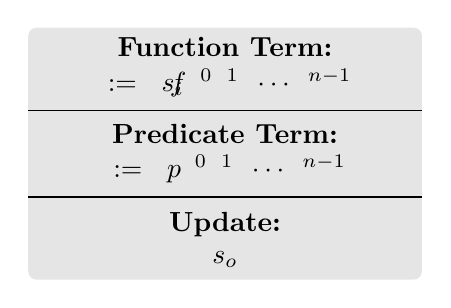
\begin{tikzpicture}

    \fill[gray!20,rounded corners=3] (-2.5,-2.5) rectangle (2.5,0.7);

    \node[anchor=center] at (0,0.45) {
      \textbf{Function Term:}
    };

    \node[anchor=center] at (0,0) {
      $ \fterm \ := \ \; \name{s}_{\name{i}} \! \! \sep \! \name{f} \ \, \fterm^{0} \
      \, \fterm^{1} \ \, \cdots \ \, \fterm^{n-1} $
    };

    \draw (-2.5,-0.35) -- (2.5,-0.35);

    \node[anchor=center] at (0,-0.65) {
      \textbf{Predicate Term:}
    };

    \node[anchor=center] at (0,-1.1) {
      $ \pterm \ := \ \;
      \name{p} \ \, \fterm^{0} \ \, \fterm^{1} \ \, \cdots \ \, \fterm^{n-1}  $
    };

    \draw (-2.5,-1.45) -- (2.5,-1.45);

    \node[anchor=center] at (0,-1.8) {
      \textbf{Update:}
    };

    \node[anchor=center] at (0,-2.25) {
      $ \upd{\name{s}_{\name{o}}}{\fterm} $
    };
  \end{tikzpicture}
  \caption{Term Definitions \mbox{\ }}
  \label{fig:termdefinitions}
\end{subfigure}

\caption{General architecture of reactive systems that are specified in TSL
  on the left, and the structure of function, predicate and updates
  on the right.}
\end{figure}

\medskip

\fussy

\noindent \textit{Function Terms, Predicate Terms, and Updates} In \TSL we
differentiate between two elements: we use purely functional
transformations, reflected by \mbox{functions~$ f \in \functions $}
and their compositions, and \mbox{predicates~$ p \in \predicates $},
used to control how data flows inside the system.
To argue about both
elements we use a term based notation, where we distinguish between
function terms~$ \fterm $ and predicate terms~$ \pterm $,
respectively. Function terms are either constructed from inputs or
cells \mbox{($ \name{s}_{\name{i}} \in \inames \cup \cells $)}, or from
functions, recursively applied to a set of function terms. Predicate
terms are constructed similarly, by applying a predicate to a set of
function terms.
%
\sloppy
%
Finally, an update takes the result of a function computation and passes it either to an output
or a cell ($ \name{s}_{\name{o}} \in \onames \cup \cells $). An overview of the syntax
of the different term notations is given in \cref{fig:termdefinitions}.
Note that we use curried argument notation similar to functional
programming languages.

We denote sets of function and predicate terms, and updates by
$ \fterms $, $ \pterms $ and $ \uterms $, respectively, where
$ \pterms \subseteq \fterms $.  We use $ \fnames $ to denote the set
of function literals and $ \pnames \subseteq \fnames $ to denote the
set of predicate literals, where the literals $ \name{s}_{\name{i}} $,
$ \name{s}_{\name{o}} $, $ \name{f} $ \linebreak and~$ \name{p} $ are
symbolic representations of inputs and cells, outputs and cells, and
functions and predicates, respectively.  Literals are used to
construct terms as shown in \cref{fig:termdefinitions}. Since we use a
symbolic representation, functions and predicates are not tied to a
specific implementation. However, we still classify them according to
their arity, i.e., the number of function terms they are applied to,
as well as by their type: input, output, cell, function or
predicate. Furthermore, terms can be compared syntactically using the
equivalence relation~$ \equiv $.  To assign a semantic interpretation
to functions, we use an assignment function
\mbox{$ \assign{\cdot} \from \fnames \to \functions $}.

\medskip

\noindent \textit{Inputs, Outputs, and Computations} We consider momentary
inputs \mbox{$ i \in \fspace{\inames}{\values} $}, which are
assignments of inputs~$ \name{i} \in \inames $ to values
$ v \in \values $. For the sake of readability let
$ \inputs = \fspace{\inames}{\values} $. Input streams are infinite
sequences~\mbox{$ \iota \in \inputs^{\hspace{0.2pt}\omega} $}
consisting of infinitely many momentary inputs.

Similarly, a momentary output~$ o \in \fspace{\onames}{\values} $ is
an assignment of outputs~$ \name{o} \in \onames $ to values
$ v \in \values $, where we also use
$ \outputs = \fspace{\onames}{\values} $. Output streams are infinite
sequences~$ \varrho \in \outputs^{\hspace{0.5pt}\omega} $. To capture
the behavior of a cell, we introduce the notion of a
computation~$ \comp $.
A computation fixes the function terms that are used to compute outputs and cell updates,
without fixing semantics of function literals.
 Intuitively, a computation only determines which
function terms are used to compute an output, but abstracts from actually
computing it.

The basic element of a computation is a computation
step~$ \cstep \in \fspace{\onames \cup \cells}{\fterms} $, which is an
assignment of outputs and
cells~$ \name{s}_{\name{o}} \in \onames \cup \cells $ to function
terms~$ \fterm \in \fterms $. For the sake of readability let
$ \comps = \fspace{\onames \cup \cells}{\fterms} $. A computation step
fixes the control flow behaviour at a single point in time. A
computation~\mbox{$ \comp \in \comps^{\omega} $} is an infinite sequence of
computation steps.

As soon as input streams, and function and predicate implementations
are known, computations can be turned into output streams. To this
end, let $ \assign{\cdot} \from \fnames \to \functions $ be some
function assignment.  Furthermore, assume that there are predefined
constants~$ \inits \in \functions \cap \values $ for every
cell~$ \name{c} \in \cells $, which provide an initial
value for each stream at the initial point in time. To receive an
output stream from a computation~$ \comp \in \comps^{\omega} $ under
the input stream $ \iota $, we use an evaluation
function~$ \eval \from \comps^{\omega} \times
\inputs^{\hspace{0.2pt}\omega} \times \dtime \times \fterms \to
\values $:
%
\begin{eqnarray*}
  \eval(\comp, \iota, t, \name{s}_{\name{i}}) & = &
    \begin{cases}
      \iota(t)(\name{s}_{\name{i}}) & \text{if } \name{s}_{\name{i}} \in \inames \\
      \initsE &
      \text{if } \name{s}_{\name{i}} \in \cells \ \wedge \ t = 0 \\
      \eval(\comp, \iota, t-1, \comp(t-1)(\name{s}_{\name{i}})) &
      \text{if } \name{s}_{\name{i}} \in \cells \ \wedge \ t > 0
    \end{cases}
  \\[0.5em]
  \eval(\comp, \iota, t, \name{f} \ \term_{0} \ \cdots \ \term_{m-1}) & = &
  \assign{\name{f}} \ \eval(\comp,\iota, t,\term_{0}) \
  \cdots \ \eval(\comp,\iota, t,\term_{m-1})
\end{eqnarray*}
%
Then
$ \varrho_{\hspace{-1pt}\langle \hspace{-1pt}\cdot
  \hspace{-1pt}\rangle \hspace{-1pt}, \comp, \iota} \in
\outputs^{\hspace{0.5pt}\omega} $ is defined via
$ \varrho_{\hspace{-1pt}\langle \hspace{-1pt}\cdot
  \hspace{-1pt}\rangle \hspace{-1pt}, \comp, \iota}(t)(\name{o}) =
\eval(\comp, \iota, t, \name{o}) $ for all $ t \in \dtime $,
$ \name{o} \in \onames $.

\medskip
\smallskip

\noindent \textit{Syntax} Every TSL formula~$ \varphi $ is built
according to the following grammar:
%
\begin{equation*}
  \varphi \ \ := \ \
  \term \in \pterms\cup \uterms
  \!\sep\! \neg \varphi
  \!\sep\! \varphi \wedge \varphi
  \!\sep\! \LTLnext \varphi
  \!\sep\! \varphi \LTLuntil \varphi
\end{equation*}
%
An atomic proposition $\tau$ consists either of a predicate term, serving as a
Boolean interface to the inputs, or of an update, enforcing a
respective flow at the current point in time. Next, we have the
Boolean operations via negation and conjunction, that allow us to express
arbitrary Boolean combinations of predicate evaluations and
updates. Finally, we have the temporal operator next:
$ \LTLnext \psi $, to specify the behavior at the next point in time
and the temporal operator until:~$ \vartheta \LTLuntil \psi $, which
enforces a property~$ \vartheta $ to hold until the property~$ \psi $
holds, where $ \psi $ must hold at some point in the future
eventually.
%
\medskip
\smallskip

\noindent \textit{Semantics} Formally, this leads to the following
semantics.  Let $ \assign{\cdot} \from \fnames \to \functions $,
\mbox{$ \iota \in \inputs^{\hspace{0.2pt}\omega} $}, and
$ \comp \in \comps^{\omega} $ be given, then the validity of a $ \TSL$
formula~$ \varphi $ with respect to $ \comp $ and $ \iota $ is defined inductively
over $ t \in \dtime $ via:
%
\begin{equation*}
  \begin{array}{lcl}
    \\[-1.8em]
    \comp, \iota, t \sats \name{p} \ \term_{0} \ \cdots \ \term_{m-1} & \ :\Leftrightarrow \ \
    & \eval(\comp,\iota,t,\name{p} \ \term_{0} \ \cdots \ \term_{m-1}) \\[0.2em]
    \comp, \iota, t \sats \upd{\name{s}}{\!\term} & :\Leftrightarrow
    & \comp(t)(\name{s}) \equiv \term \\[0.2em]
    \comp, \iota, t \sats \neg \psi & :\Leftrightarrow
    & \comp, \iota, t \nsats \psi \\[0.2em]
    \comp, \iota, t \sats \vartheta \wedge \psi & :\Leftrightarrow
    & \comp, \iota, t \sats \vartheta \ \wedge \ \comp, \iota, t \sats \psi \\[0.2em]
    \comp, \iota, t \sats \LTLnext \psi & :\Leftrightarrow
    & \comp, \iota, t+1 \sats \psi \\[0.2em]
    \comp, \iota, t \sats \vartheta \LTLuntil \psi & :\Leftrightarrow
    & \exists t'' \geq t. \ \
         \forall t \leq t' < t''. \ \ \comp, \iota, t' \sats \vartheta \ \,
         \wedge \ \, \comp, \iota, t'' \sats \psi
  \end{array}
\end{equation*}
%
Consider that the satisfaction of a predicate depends on the current
computation step and the steps of the past, while for updates it only
depend on the current computation step. Furthermore, updates are only
checked syntactically, while the satisfaction of predicates depends on
the given assignment~$ \assign{\cdot} $ and the input stream
$ \iota $.
%
We say that $ \comp $ and $ \iota $ satisfy $ \varphi $, denoted by
$ \comp, \iota \sats \varphi$, if $ \comp, \iota, 0 \sats \varphi
$.

Beside the basic operators we have the standard derived Boolean
operators, as well as the derived temporal operators:
\textit{release}~$ \varphi \LTLrelease \psi \equiv \neg ((\neg \psi)
\LTLuntil (\neg \varphi)) $,
\textit{finally}~$ \LTLfinally \varphi \equiv \emph{true} \LTLuntil
\varphi $,
\textit{always}~$ \LTLglobally \varphi \equiv \emph{false} \LTLrelease
\varphi $, the \textit{weak} version of \textit{until}
$ \varphi \LTLweakuntil \psi \equiv (\varphi \LTLuntil \psi) \vee
(\LTLglobally \varphi) $, and \textit{as soon
  as}~$ \varphi \mathop{\mathcal{A}}\hspace{0.5pt} \psi \equiv \neg
\psi \LTLweakuntil (\psi \wedge \varphi) $.

\medskip

\noindent \textit{Realizability} We are interested in the following
realizability problem: given a $ \TSL $ formula~$ \varphi $, is there
a strategy~$ \sigma \in \fspace{\inputs^{+}}{\comps} $ such that for every
input $ \iota \in \inputs^{\omega} $ and function implementation
$ \assign{\cdot} \from \fnames \to \functions $, the branch
$ \branch{\sigma}{\iota} $ satisfies $ \varphi $, i.e.,
%
\begin{equation*}
  \exists \sigma \in \fspace{\inputs^{+}}{\comps}. \ \, \forall \iota \in \inputs^{\hspace{0.2pt}\omega}. \ \, \forall \assign{\cdot} \from
  \fnames \to \functions. \ \, \branch{\sigma}{\iota}, \iota \sats \varphi
\end{equation*}
%
If such a strategy~$ \sigma $ exists, we say $ \sigma $ realizes
$ \varphi $. If we additionally ask for a concrete instantiation of
$ \sigma $, we consider the synthesis problem of TSL.


\section{TSL Properties}
\label{sec:props}
In order to synthesize programs from TSL specifications, we give an overview of the first part of our synthesis process, as shown in \cref{fig:system}.
First we show how to approximate the semantics of TSL through a reduction to LTL.
However, due to the approximation, finding a realizable strategy immediately may fail.
Our solution is a CEGAR loop that improves the approximation.
This CEGAR loop is necessary, because the realizability problem of TSL is undecidable in general.

\medskip

\noindent \textit{Approximating TSL with LTL} We approximate TSL
formulas with weaker LTL formulas.  The approximation reinterprets the
syntactic elements, $\pterms$ and $\uterms$, as atomic propositions
for LTL. This strips away the semantic meaning of the function
application and assignment in TSL, which we reconstruct by later
adding assumptions lazily to the LTL formula.

Formally, let $ \pterms $ and $ \uterms $ be the finite sets of
predicate terms and updates, which appear in
$ \varphi_{\textit{TSL}} $, respectively. For every assigned signal, we
partition $ \uterms $ into
$ \biguplus_{\name{s}_{\name{o}} \in \onames \cup \cells}
\uterms^{\hspace{0.5pt}\name{s}_{\name{o}}} $. For every
$ \name{c} \in \cells $ let \mbox{$\utermsp^{\hspace{0.5pt}\name{c}} =
  \uterms^{\hspace{0.5pt}\name{c}} \cup \set{ \upd{\name{c}}{\name{c}}
  } $}, for $ \name{o} \in \onames $ let
$ \utermsp^{\hspace{0.5pt}\name{o}} = \uterms^{\hspace{0.5pt}\name{o}}
$, and let
$ \utermsp = \bigcup_{\name{s}_{\name{o}} \in \onames \cup \cells}
\utermsp^{\hspace{0.5pt}\name{s}_{\name{o}}} $.  We construct the LTL
formula~$ \varphi_{\textit{LTL}} $ over the input
propositions~$ \pterms $ and output propositions $ \utermsp $ as
follows:
%
\begin{equation*}
  \varphi_{\textit{LTL}} \, = \;
  \LTLglobally \Big ( \bigwedge_{\name{s}_{\name{o}} \in \onames \cup \cells} \,
  \bigvee_{\term \in \utermsp^{\hspace{0.5pt}\name{s}_{\name{o}}}}
  \big( \term \; \wedge \bigwedge_{\term' \in
    \utermsp^{\hspace{0.5pt}\name{s}_{\name{o}}} \setminus
    \set{ \term }} \neg \, \term' \big)  \Big) \ \wedge \
  \textsc{SyntacticConversion}\big(\varphi_{\textit{TSL}}\big)
\end{equation*}
%
Intuitively, the first part of the equation partially reconstructs the semantic meaning of updates by ensuring that a signal is not updated with multiple values at a time.
The second part extracts the reactive constraints of the TSL formula without the semantic meaning of functions and updates.
%
\begin{theorem}
  \label{thm:tsl2ltl} If $ \varphi_{\textit{LTL}} $ is realizable, then $ \varphi_{\textit{TSL}} $ is realizable.
\end{theorem}
%
\noindent The proof of \cref{thm:tsl2ltl} is given in \cref{proof:tsl2ltl}.
Note that unrealizability of $\varphi_{\textit{LTL}} $ does not imply that $ \varphi_{\textit{TSL}}$ is unrealizable.
It may be that we have not added sufficiently many environment assumptions to the approximation in order for the system to produce a realizing strategy.

\medskip

\label{ex:asLTL}

\begin{figure*}[t]
    \centering
    \begin{subfigure}[t]{0.28\textwidth}
      \centering
      $ \begin{array}{c}
          \\[-0.5em]
          \LTLglobally \; (\upd{\name{y}}{\name{y}} \, \vee \, \upd{\name{y}}{\name{x}}) \\[0.2em]
          \wedge \ \LTLeventually \, \name{p} \ \name{x} \, \impl \,
          \LTLeventually \, \name{p}\ \name{y} \\[-0.5em]
          \
        \end{array} $
        \caption{TSL specification}
\label{eq:tslSimple}
    \end{subfigure}%
    ~ ~
    \begin{subfigure}[t]{0.30\textwidth}
      \centering
      $ \begin{array}{c}
          \LTLglobally \; \neg ( \name{y\_to\_y} \, \wedge \, \name{x\_to\_y}) \\[0.2em]
          \wedge \ \LTLglobally \; (\name{y\_to\_y} \, \vee \, \name{x\_to\_y}) \\[0.2em]
          \wedge \ \LTLeventually \, \name{p\_x} \, \impl \
          \LTLeventually \, \name{p\_y}
        \end{array} $
\caption{initial approximation}
\label{eq:ltlSimple}
    \end{subfigure}%
    ~\;
    \begin{subfigure}[t]{0.35\textwidth}
      \centering
      \vspace{-1em}
  \begin{tikzpicture}[->,>=stealth',shorten >=1pt,auto,node distance=2.8cm,initial text=]
    \tikzstyle{every state}=[fill=blue!20,draw,text=white,minimum size=1.5em]
    \node[initial,state] (A)                    {};
    \path (A) edge [loop right] node {$\name{p\_x} \; \wedge \; \neg \, \name{p\_y}$} (A);
  \end{tikzpicture}
  \vspace{1.1em}
\caption{spurious counter-strategy}
\label{eq:tslSimpleSoln}
    \end{subfigure}
    \caption{
      A TSL specification~(a) with input~\name{x} and cell~\name{y} that is realizable. A winning strategy is to save~\name{x} to \name{y} as soon as $ \name{p}(\name{x}) $ is satisfied. However, the initial approximation~(b), that is passed to an LTL synthesis solver, is unrealizable, as proven through the counter-strategy~(c) returned by the LTL solver.}
    \label{fig:approx}
\end{figure*}

\noindent \textit{Example} As an example, we present a simple TSL specification in \cref{eq:tslSimple}.
The specification asserts that the environment provides an input~\name{x} for which the predicate~$ \name{p}~\name{x} $ will be satisfied eventually. The system must guarantee that eventually $ \name{p}~\name{y} $ holds.
According to the semantics of TSL the formula is realizable. The system can take the value of $ \name{x} $ when $ \name{p}~\name{x} $ is true and save it to $ \name{y} $, thus guaranteeing that $ \name{p}~\name{y} $ is satisfied eventually.
This is in contrast to LTL, which has no semantics for pure functions - taking the evaluation of $ \name{p}~\name{y} $ as an environmentally controlled value that does not need to obey the consistency of a pure function.

\medskip

\noindent \textit{Refining the LTL Approximation} It is possible that the LTL solver returns a counter-strategy for the environment although the original TSL specification is realizable.
We call such a counter-strategy \textit{spurious} as it exploits the additional freedom of LTL to violate the purity of predicates as made possible by the underapproximation.
Formally, a counter-strategy is an infinite tree $ \pi \from \comps^{*} \to 2^{\pterms} $, which provides predicate evaluations in response to possible update assignments of function terms~$ \fterm \in \fterms $ to outputs~$ \name{o} \in \onames $.
W.l.o.g.\ we can assume that $ \onames $, $ \fterms $ and $ \pterms $ are finite, as they can always be restricted to the outputs and terms that appear in the formula.
A counter-strategy is spurious, iff there is a branch~$ \branch{\pi}{\comp} $ for some computation~$ \comp \in \comps^{\omega} $, for which the strategy chooses an inconsistent evaluation of two equal predicate terms at different points in time, i.e.,
%
\begin{equation*}
  \begin{array}{l}
    \exists \comp \in \comps^{\omega}. \ \exists t, t' \in \dtime. \ \exists \pterm \in \pterms. \\[0.2em]
    \qquad \pterm \in \pi(\comp(0)\comp(1)\ldots\comp(t-1)) \, \wedge \, \pterm \notin \pi(\comp(0)\comp(1)\ldots\comp(t'-1)) \ \wedge \\[0.2em]
    \qquad \forall \assign{\cdot} \from \fnames \to \functions. \ \eval(\comp, \branch{\pi}{\comp}, t, \pterm) \, = \, \eval(\comp, \branch{\pi}{\comp}, t', \pterm).
  \end{array}
\end{equation*}
%
Note that a non-spurious strategy can be inconsistent along multiple
branches. Due to the definition of realizability
the environment can choose function and
predicate assignments differently against every system strategy
accordingly.

By purity of predicates in TSL the environment is forced to
always return the same value for predicate evaluations on equal
values. However, this semantic property cannot be enforced implicitly
in LTL.  To resolve this issue we use the returned counter-strategy to
identify spurious behavior in order to strengthen the LTL
underapproximation with additional environment assumptions.
After adding the derived assumptions, we re-execute the LTL synthesizer to check whether the
added assumptions are sufficient in order to obtain a winning strategy
for the system.  If the solver still returns a spurious strategy, we
continue the loop in a CEGAR fashion until the set of added
assumptions is sufficiently complete.  However, if a non-spurious strategy is
returned, we have found a proof that the given
TSL specification is indeed unrealizable and terminate.

\goodbreak

\begin{algorithm}[t]
  \small
  \caption{Check-Spuriousness} \label{alg:spurious}
  \begin{algorithmic}[1]
    \Require{bound~$ b $, counter-strategy~$ \pi \from \comps^{*}\!\! \to \! 2^{\pterms} $ (finitely represented using $ m $ states)}

    \vspace{0.3em}

    \ForAll{$ v \in \comps^{m \cdot b},\, \pterm \in \pterms, \, t,t' \in \set{ 0,1,\ldots,m\cdot b - 1} $}
      \If{$ \evalid(v,\iota_{\name{id}},t,\pterm) \equiv \evalid(v,\iota_{\name{id}},t',\pterm) \wedge \mbox{\qquad} \qquad \qquad \qquad \qquad \qquad \qquad \qquad $ $ \mbox{\ }\hspace{2.5em} \pterm \in \pi(v_{0}\ldots v_{t-1}) \wedge \pterm \notin \pi(v_{0}\ldots v_{t'-1}) $}
      \State \quad $ w \gets \texttt{reduce}\,(v,\pterm,t,t') $
      \State \quad {\textbf{return} \ $ \LTLglobally \big(\! \bigwedge_{i=0}^{t-1} \LTLnext^{i}\! w_{i} \, \wedge \, \bigwedge_{i = 0}^{t'-1} \LTLnext^{i}\! w_{i} \,\rightarrow\, (\LTLnext^{t}\! \pterm \leftrightarrow \LTLnext^{t'} \!\! \pterm) \big) $}
      \EndIf
    \EndFor
    \State {\textbf{return} \ \texttt{``non-spurious''}}
  \end{algorithmic}
  \vspace{-0.2em}
\end{algorithm}

\cref{alg:spurious} shows how a returned counter-strategy~$ \pi $ is
checked for being spurious. To this end, it is sufficient to
check~$ \pi $ against system strategies bounded by the given
bound~$ b $, as we use bounded
synthesis~\cite{Schewe:2013}. Furthermore, we can assume w.l.o.g.\
that~$ \pi $ is given by a finite state representation, which is
always possible due to the finite model guarantees of LTL. Also note
that~$ \pi $, as it is returned by the LTL synthesizer, responses to
sequences of sets of updates~$ (2^{\utermsp})^{*} $. However, in our
case $ (2^{\utermsp})^{*} $ is an alternative
representation~of~$ \comps^{*} $, due to the additional constraints
added during the construction~of~$ \varphi_{\textit{LTL}} $.

The algorithm iterates over all possible
responses~$ v \in \comps^{m \cdot b} $ of the system up to depth
$ m \cdot b $. This is sufficient, since any deeper exploration would
result in a state repetition of the cross-product of the finite state
representation of~$ \pi $ and any system strategy bounded by~$ b
$. Hence, the same behaviour could also be generated by a smaller
sequence. At the same time, the algorithm iterates over
predicates~$ \pterm \in \pterms $ appearing in
$ \varphi_{\textit{TSL}} $ and times $ t $ and $ t' $ smaller
than~$ m \cdot b $. For each of these elements, spuriousness is
checked by comparing the output of~$ \pi $ for the evaluation of
$ \pterm $ at times~$ t $ and $ t' $, which should only
differ, if the inputs to the predicates are different as well. This
can only happen, if the passed input terms have been constructed
differently over the past. We check it by using the evaluation
function~$ \eta $ equipped with the identity assignment
$ \assign{\cdot}_{\texttt{id}} \from \fnames \to \fnames $, with
$ \assign{\name{f}}_{\texttt{id}} = \name{f} $ for all
$ \name{f} \in \fnames $, and the input sequence
$ \iota_{\texttt{id}} $, with
$ \iota_{\texttt{id}}(t)(\name{i}) = (t,\name{i}) $ for all
$ t \in \dtime$ and $ \name{i} \in \inames $, that always generates a
fresh input. Syntactic inequality of
$ \evalid(v,\iota_{\name{id}},t,\pterm) $ \linebreak and
$ \evalid(v,\iota_{\name{id}},t',\pterm) $ then is a sufficient
condition for the existence of an assignment
$ \assign{\cdot} \from \fterms \to \functions $, for which $ \pterm $
evaluates differently at times $ t $ and~$ t' $.

If spurious behaviour of~$ \pi $ could be found, then the revealing
response~$ v \in \comps^{*} $ is first simplified using
$ \texttt{reduce} $, which turns $ v $ back to a sequence of sets of
updates~$ w \in (2^{\utermsp})^{*} $ and removes updates that do not
affect the behavior of $ \pterm $ at the times $ t $ and $ t' $ to
accelerate the termination of the CEGAR loop. Afterwards, the
sequence~$ w $ is turned into a new assumption that prohibits the found
spurious behavior and, thus, further refines the LTL
underapproximation.

As an example of this process, reconsider the spurious
counter-strategy of \cref{eq:tslSimpleSoln}. Already after the first
system response~$ \upd{\name{y}}{\name{x}} $, the environment produces
an inconsistency by evaluating~$ \name{p} \ \name{x} $ and
$ \name{p} \ \name{y} $ differently. This is inconsistent, as the
cell~$ \name{y} $ holds the same value at time~$ t = 1 $ as the
input~$ \name{x} $ at time~$ t = 0 $. Using \cref{alg:spurious} we generate
the new
assumption~$ \LTLglobally (\upd{\name{y}}{\name{x}} \impl (\name{p} \
\name{x} \leftrightarrow \LTLnext \name{p} \ \name{y})) $. After adding this
strengthening the LTL synthesizer returns a realizability result.

\medskip

\goodbreak

\noindent \textit{Undecidability}
Although we can approximate the semantics of TSL with LTL, there are
TSL formulas that cannot be expressed as LTL formulas of finite
size.
%
\begin{theorem}\label{thm:decidability}
  The realizability problem of $ \TSL $ is undecidable.
\end{theorem}
%
\begin{proof}
  We reduce an instance of the Post Correspondence
  Problem~(PCP)~\cite{post1946}, consisting of an alphabet~$ \Sigma $
  and sequences
  $ w_{0}w_{1}\ldots w_{n}, v_{0}v_{1}\ldots v_{n} \in \Sigma^{*} $,
  to the realizability of a $ \TSL $ formula~$ \varphi $. To this end,
  we fix some unary predicate~$ \name{p} \in \pnames $, a~unary
  function $ \name{f} \in \fnames $ for every alphabet symbol
  $ f \in \Sigma $, and some $ 0 $-nary
  function~$ \name{X} \in \fnames $. The system has no
  inputs~$ \inames $, but two outputs $ \name{A} \in \onames $ and
  $ \name{B} \in \onames $.

  Initially, we assign the signals $ \name{A} $ and $ \name{B} $ the
  constant value~$ \name{X} $. From then on, we non-deterministically
  pick pairs $ (w_{j},v_{j}) $ in every time step, as provided by the
  PCP instance, where every $ w_{j} $ and $ v_{j} $ is represented as
  a stacked composition of the corresponding alphabet functions. Our
  choice is stored in the signals~$ \name{A} $ and $ \name{B} $ for
  $ w_{j} $ and $ v_{j} $, respectively. Finally, we check that the
  sequences of function applications, constructed over time, are equal
  at some point, using the eventually operator~$ \LTLfinally $ and the
  universally quantified predicate~$ \name{p} $ to check for equality.
\end{proof}
%
\noindent A more detailed version of the proof can be found in
\cref{proof:decidability}. Also note that no inputs are used by
the proof, which additionally shows that the \mbox{``satisfiability''} problem of
\TSL is undecidable as well.


\section{TSL Synthesis}
\label{sec:synth}
Our synthesis framework provides a modular refinement process
to synthesize executables from $ \TSL $ specifications, as depicted
in \cref{fig:system}. The user initially provides a
$ \TSL $ specification over predicate and function terms.  At the end
of the procedure, the user receives an executable to control a
reactive system.

The first step of our method answers the synthesis question of TSL: if
the specification is realizable, then a control flow model is
returned.  To this end, an intermediate translation to LTL is used,
utilizing an LTL synthesis solver that produces circuits in the AIGER
format. If the specification is realizable, the resulting control flow
model is turned into Haskell code, which is implemented as an
independent Haskell module. The user has the choice between two
different targets: a module built on Arrows, which is compatible with
any Arrowized FRP library, or a module built on Applicative, which
supports Applicative FRP \mbox{libraries}. Our procedure generates a single
Haskell module per TSL specification. This makes naturally decomposing
a project according to individual tasks possible. Each module provides
a single component, which is parameterized by their initial state and
the pure function and predicate transformations. As soon as these are
provided as part of the surrounding project context, a final
executable can be generated by compiling the Haskell code.

An important feature of our synthesis approach is that implementations
for the terms used in the specification are only required after
synthesis.  This allows the user to explore several possible
specifications before deciding on any term implementations.

\paragraph{Control Flow Model} The first step of our approach is the
synthesis of a \textit{Control Flow Model}~$ \cfm $ (CFM) from the
given $ \TSL $ specification~$ \varphi $, which provides us with a
uniform representation of the control flow structure of our final
program.

\noindent Formally, a CFM~$ \cfm $ is a tuple
$ \cfm = (\inames, \onames, \cells, \vertices, \labeling,
\dependencies), $ where $ \inames $ is a finite set of inputs,
$ \onames $ is a finite set of outputs, $ \cells $ is a finite set of
cells, $ \vertices $ is a finite set of vertices,
$ \labeling \from \vertices \to \fnames $ assigns a
vertex a function~$ \name{f} \in \fnames $ or a
predicate~$ \name{p} \in \pnames $, and
%
\begin{equation*}
  \dependencies \from (\onames \cup \cells \cup \vertices) \times
  \nats \to (\inames \cup \cells \cup \vertices \cup \set{ \bot })
\end{equation*}
%
is a dependency relation that relates every output, cell, and
vertex of the CFM with $ n \in \nats $ arguments, which are either
inputs, cells, or vertices. Outputs and
cells~$ \name{s} \in \onames \cup \cells $ always have only a single
argument, i.e., $ \delta(s, 0) \not\equiv \bot $ and
\mbox{$ \forall m > 0 .\ \delta(\name{s}, m) \equiv \bot $}, while for
vertices~$ x \in \vertices $ the number of arguments $ n \in \nats $
align with the arity of the assigned function or predicate
$ \labeling(x) $, i.e.,
$ \forall m \in \nats .\ \delta(s, m) \equiv \bot \leftrightarrow m >
n $. A CFM is valid if it does not contain circular dependencies,
i.e., on every cycle induced by $ \delta $ there must lie at least a
single cell. We only consider valid CFMs.

\input{musicFRP}

An example CFM for our music player of \cref{sec:motiv} is depicted in
\cref{fig:cfmexample}. Inputs~$ \inames $ come from the left
and outputs~$ \onames $ leave on the right. The example
contains a single cell~$ \name{c} \in \cells $, which holds the
stateful memory~\name{Cell}, introduced during synthesis for the
module. The green, arrow shaped boxes depict vertices~$ \vertices $,
which are labeled with functions and predicates names, according
to~$ \labeling $. For the Boolean decisions that define $\delta$, we use circuit symbols for
conjunction, disjunction, and negation. Boolean decisions are piped to
a multiplexer gate that selects the respective
update streams. This allows each update stream to be passed to an output stream if and only if the
respective Boolean trigger evaluates positively, while
our construction ensures mutual exclusion on the Boolean triggers. For
code generation, the logic gates are implemented using the corresponding dedicated Boolean functions.
After building a control structure, we assign semantics to functions
and predicates by providing implementations.  To this end, we use
Functional Reactive Programming (FRP).  Prior work has established
Causal Commutative Arrows (CCA) as an FRP language pattern equivalent
of a CFM~\cite{jfp/LiuCH11,liu2007plugging,yallop2016causal}.  CCAs
are an abstraction subsumed by other functional reactive programming
abstractions, such as Monads, Applicative and
Arrows~\cite{jfp/LiuCH11,lindley2011idioms}.
There are many FRP libraries using
Monads~\cite{elm,hudakFRAN,ploeg2015frpnow},
Applicative~\cite{reactivebanana,clash2015,helbling2016juniper,Reflex},
or Arrows~\cite{courtney2003yampa,murphy2016livefrp,perez2016yampa,UISF},
and since every Monad is also an Applicative and Applicative/Arrows both are universal design patterns, we can give uniform
translations to all of these libraries using translations to just Applicative
and Arrows. Both translations are possible due to the flexible notion of a CFM.

In the last step, the synthesized FRP program is compiled into an
executable, using the provided function and predicate
implementations. This step is not fixed to a single
compiler implementation, but in fact can use any FRP compiler (or
library) that supports a language abstraction at least as expressive as CCA.
For example, instead of creating an Android music player app, we could
target an FRP web interface~\cite{Reflex} to create an online music
player, or an embedded FRP library~\cite{helbling2016juniper} that
allows us to directly instantiate the player on a computationally more
restricted device. By using the strong core of CCA, we even can go
down the whole chain and directly implement the player in hardware,
which is for example possible with the C$ \lambda $aSH  compiler~\cite{clash2015}.
Note that we still need to give separate implementations for the functions and
predicates for each target. However, our specification and the
synthesized CFM always stay the same.


\section{Experimental Results}
\label{sec:eval}
\section{Evaluation}

We evaluate \system in two aspects: (1) \emph{effectiveness (accuracy)}, which assesses how accurate \system is in  detecting and ranking root causes, and (2) \emph{efficiency}, which assesses how long it takes for \system to derive root causes and conduct end-to-end analysis in action. Particularly, we intend to address the following research questions:
    %\item \emph{User Experience}, which represents how two groups of SREs experience while using \system: domain SREs which use \system to find the root cause to investigate and mitigate, infrastructure SREs which maintain \system to facilitate new requirements.


\begin{itemize}
    \item \textbf{RQ1.} What are the accuracy and efficiency of \system when applied on the collected dataset?
    \item \textbf{RQ2.} How does \system compare with baseline approaches in terms of accuracy?
    \item \textbf{RQ3.} What are the accuracy and efficiency of \system in an end-to-end scenario?
\end{itemize}

% RQ1 aims to see if given a clear triggering event, how would \system perform. RQ2 aims to see whether using adaptive event-driven approach has an advantage compared to baseline in this scenario. RQ3 puts \system in the real time end-to-end scenario, evaluates the \system's efficiency as a whole. 
%2) Conduct a user study to figure out whether \system is actually helpful and user-friendly to the end SRE users.

\subsection{Evaluation Setup}
\label{sec:evalset}
%To measure whether \system can deal with the challenges with industrial settings, we evaluate \system in an environment that is able to represent the real-time large scale distributed system that is running in real world
To evaluate \system in a real-world scenario, we deploy and apply \system  in eBay's e-commerce system that serves more than 159 million active buyers. In particular, we apply \system upon a microservice ecosystem that contains over 5,000 services on three data centers. These services are built on different tech stacks with different programming languages, including Java, Python, Node.js, etc. Furthermore, these services interact with each other by using different types of service protocols, including HTTP, gRPC,  and Message Queue. The distributed tracing of the ecosystem generates 147B traces on average per day.% with 2.8T spans~\cite{opentracing}%The most busy services in the system have more than 50,000 TPS (transactions per second) every day. It is both time-consuming and troublesome for site reliability engineers to manually solve different incidents without the support of tools like \system.  
\subsubsection{Data Set}
\label{sec:dataset}
The SRE teams at eBay help collect a labeled data set containing 952 incidents over 15 months (Jan 2020 - Apr 2021). Each incident data contains the input required by \system (e.g., dependency snapshot and events with details) and the root cause manually labeled by the SRE teams. %To create this data set, 
These incidents are grouped into two categories: 
%we evaluate over 1,500 incidents grouped into two categories: %and around ${40\%}$ cases are missing supported events or caused by external issues (e.g, regional network provider failures). These incidents are categorized as:
\begin{itemize}
\item \emph{Business domain incidents.} These incidents are detected mainly due to their business impact. For example, end users encounter failed interactions, and business or customer experience is impacted, similar to the example in  Figure~\ref{fig:example1}. 
\item \emph{Service-based incidents.} These incidents are detected mainly due to their impact on the service level, similar to the example in Figure~\ref{fig:dynamic_example}.
\end{itemize}

An internal incident may get detected early, and then likely get categorized as a service-based incident or even solved directly by owners without records. On the other hand, infrastructure-level issues or issues of external service providers (e.g., checkout and shipping services) may not get detected until business impact is caused. 

There are 782 business domain incidents and 170 service-based incidents in the data set. For each incident, the root cause is manually labeled, validated, and collected by the SRE teams, who handle the site incidents everyday. For a case with multiple interacting causes, only the most actionable/influential event is labelled as the root cause for the case. These actual root causes and incident contexts serve as the ground truth in our evaluation.


%To trigger the root cause analysis, w
%\begin{enumerate}
%\item\textbf{Business Monitoring}: Business metrics alerts are collected from here. There are around 200+ business time series are detected  by  anomaly detection service every minute.
%\item\textbf{Application Monitoring}:Different application alerts including TPS alerts, Error Spiking alerts, Latency alerts are collected from here. There are around several million time series are detected by  anomaly detection service every minute. 
%\item\textbf{Load Balance Monitoring}: VIP connection number spiking alerts are collected from here. There are around 60k time series are detected by  anomaly detection service every 5 secs. 
%\item\textbf{Deployment system}: Deployment events are collected from here.
%\item\textbf{Site Event system}: Application mark down events and DB mark down events  are collected from here. When a micro-service is not able to talk to its downstream service after retries, it will mark down the downstream service and send a service mark down event to site event system.  Similar to this, when a micro-service is not able to talk to Database, it will mark down the Database and send a DB mark down event to site event system.
%\end{enumerate}

%\subsubsection{Root cause distribution of collected cases}

%\begin{figure}[t]
%\centering
%  \includegraphics[width=\columnwidth]{figures/app_rootcause.png}
%  \caption{Ground-truth RCA distribution of Application-based anomalies}
%  \label{fig:app_rootcause}
%\end{figure}
%\begin{figure}[t]
%\centering
%  \includegraphics[width=\columnwidth]{figures/biz_rootcause.png}
%  \caption{Ground-truth RCA distribution of Business domain anomalies}
%  \label{fig:biz_rootcause}
%\end{figure}

%Figure ~\ref{fig:app_rootcause} and Figure ~\ref{fig:biz_rootcause} shows the root cause distribution of application-based and business domain anomalies in the dataset. From these two charts, we can see that distribution among application-based anomalies is quite diverse while in business domain anomalies, more than 70\% of the anomalies are due to third party errors. We think this imbalance of the distribution among two categories are due to the reason that we cannot monitor third party applications like we do on other parts of the system. So that in the well-monitored applications, the anomalies would be detected earlier by the abnormal metrics before resulting in severe business impact.



\subsubsection{\system Setup}

The \system production system is deployed as three microservices and federated in three data centers with nine 8-core CPUs, 20GB RAM pods each on Kubernetes.

% They are hosted by Gunicorn to scale up. Nginx is used as our routing manager to serve static files and reverse proxying to Gunicorn, and Supervisor to watch the Gunicorn servers in the background and start the processes on reboot.

\subsubsection{Baseline Approaches} 
\label{sec:baseline}
In order to compare \system with other related approaches, we design and implement two baseline approaches for the evaluation:  
\begin{itemize}
    \item \emph{Naive Approach.} This approach directly uses the constructed service dependency graph (Section~\ref{sec:appgraph}). The events are assigned a score by the severeness of the associated anomaly. Then a normalized score for each service is calculated summarizing all the events related to the service. Lastly, the PageRank algorithm is used to calculate the root cause ranking. 
    \item \emph{Non-adaptive Approach.} This approach is not context-aware. It replaces all special rules (i.e., conditional and dynamic ones) with their basic rule versions. Its other parts are identical to \system.
\end{itemize}
The non-adaptive approach can be seen as a baseline for reflecting a group of graph-based approaches (e.g.,  CauseInfer~\cite{chen2014causeinfer} and Microscope~\cite{lin2018microscope}). These approaches also specify certain service-level metrics but lack the context-aware capabilities of \system. Because the tools for these approaches are not publicly available, we implement the non-adaptive approach to approximate these approaches.%of existing graph-based approaches.

\subsection{Evaluation Results}

%Under the settings described in Section~\ref{sec:evalset}, we would be able to evaluate the efficiency and effectiveness of \system in real world scenarios. 

\subsubsection{RQ1}

\label{sec:rq1}

\begin{table}[t]
\centering
\caption{Accuracy of RCA by \system and baselines}
\resizebox{0.9\linewidth}{!}{ 
\begin{tabular}{l|r|r|r|r|r|r|}
\cline{2-7}
                                    & \multicolumn{2}{c|}{\system} & \multicolumn{2}{c|}{Naive} & \multicolumn{2}{c|}{Non-adaptive} \\ \cline{2-7} 
                                    & Top 3        & Top 1       & Top 3         & Top 1      & Top 3         & Top 1 \\ \hline
\multicolumn{1}{|c|}{Service-based}    & 92\%         & 74\%         & 25\%          & 16\%   & 84\% & 62\%       \\ \hline
\multicolumn{1}{|c|}{Business domain} & 96\%         & 81\%        & 2\%          & 1\%   & 28\% & 26\%       \\ \hline
\multicolumn{1}{|c|}{Combined} & 95\%         & 78\%        & 6\%          & 3\%   & 38\% & 33\%       \\ \hline
\end{tabular}
}
 \label{tab:accuracy}
  \vspace{-3.0ex} 
\end{table}

%\begin{figure}[t]
%\centering
%  \includegraphics[width=0.5\textwidth]{figures/app_wrongcause.png}
%  \caption{Ground-truth RCA distribution of Application-based anomalies which \system gives incorrect top-1 result}
%  \label{fig:app_wrongcause}
%\end{figure}
%\begin{figure}[t]
%\centering
%  \includegraphics[width=\columnwidth]{figures/biz_wrongcause.png}
%  \caption{Ground-truth RCA distribution of Business domain anomalies which \system gives incorrect top-1 result}
%  \label{fig:biz_wrongcause}
%\end{figure}

Table~\ref{tab:accuracy} shows the results of applying \system on the collected data set. We measure both top-1 and top-3 accuracy. The top-1 and top-3 accuracy is calculated as the percentage of cases where their ground-truth root cause is ranked within top 1 and top 3, respectively, in \system's results. %All joint rankings must be untied first for fairness. 
\system achieves high accuracy on both incident categories. For example, for business domain incidents, \system achieves 96\% top-3 accuracy.

% While after the causal links construction, the average number of services that are potentially targeted as root cause is reduced to 11.2 and 7.3 for service-based and business domain incidents respectively.
The unsuccessful cases that \system ranks the root cause after top 3 are mostly caused by missing event(s). %Therefore the causality graph is short of necessary causal link(s) or the root cause itself. 
More than one-third of these unsuccessful cases have been addressed by adding necessary events and corresponding rules over time. For example, initially, we had only an event type of general error spike, which mixes different categories of errors and thus causes high false-positive rate. We then have designed different event types for each category of the error metrics (including various internal and client API errors). %We include these cases to reflect a fair setting in production. 
In many cases that \system ranks the root cause after top 1, the labeled root cause is just one of the multiple co-existing root causes. But for fairness,  the SRE teams label only a single root cause in each case. According to the feedback from the SRE teams, \system still facilitates the RCA process for these cases.   %the RCA distribution of these incidents is quite different from the overall ground-truth RCA distribution. More specifically, we find that 

%Every second of an incident RCA process is valuable. 
Our results show that the runtime cost of applying \system is relatively low. For a service-based incident, the average runtime cost of \system is 1.06s while the maximum is 1.69s. For a business domain incident, the average runtime cost is 0.98s while the maximum is 1.14s. %We designed every step as lightweight as possible, for providing timely results in action.
%In order to answer RQ1, we take 219 real production incidents in eBay: 90 App-Search and 129 Domain-Search cases. These cases are handled by the site reliability engineering team or the technical duty officers of eBay. The app-search cases are from the production environment where the trigger anomaly was firstly observed at the application level. The domain-search is built for the most critical business domain - checkout flow. The trigger anomaly of domain search are generated by our ML anomaly detection systems which calculated from different business metrics and customer interaction metrics. Every root cause is manually labeled, and also collect application graph and event context for each ticket. 

%The results are present in table \ref{tab:accuracy}: The \system detects and ranked 100\% and 86\% correct root cause as Top Rank or Top 3 for app-search use cases. For Domain-search are 91\% (Top 1) and 87\% (Top 3). Obviously, our approach is significantly better than the baseline approach. Moreover, the validation for the baseline approach is less strict, the detection is at the application level. For \system accuracy we also restrict on providing the correct root cause event (e.g., code deploy).      

\subsubsection{RQ2}

\label{sec:rq2}

We additionally apply the baseline approaches on the  data set. Table~\ref{tab:accuracy} also shows the evaluation results. The results show that the accuracy of \system is substantially higher than that of the baseline approaches. In terms of the top-1 accuracy, \system achieves 78\% compared with 3\% and 33\% of the naive and non-adaptive approaches, respectively.  In terms of the top-3 accuracy, \system achieves 95\% compared with 6\% and 38\% of the naive and non-adaptive approaches, respectively. 
%In general, \system is 75\% and 45\% more, respectively, in the top-1 accuracy compared with the naive and non-adaptive baselines. \system has even larger advantages in the top-3 accuracy, being 89\% and 57\% more, respectively, compared with the two baselines. For example, \system achieves 81\% in the top-1 accuracy compared with 26\% accuracy of the non-adaptive approach for business domain incidents.%, so that SREs can save time from investigating unrelated services or events.

The naive approach performs worst in all settings, because it blindly propagates the score at service levels.
The accuracy of the non-adaptive approach is much worse for business domain incidents. The reason is that for a business domain incident, it often takes a longer propagation path since the incident is triggered by a group of services, and new dynamic dependencies may be introduced during the event collection, causing more inaccuracy for the non-adaptive approach. %As showed in Section~\ref{sec:rq1}, the causality construction helps to locate the root cause more effectively.  
There can be many non-critical or irrelevant error events in an actual production scenario, aka ``soft'' errors. We suspect that these non-critical or irrelevant events may be ranked higher by the non-adaptive approach since they are similar to injected faults and hard to be distinguished from the actual ones. \system uses dynamic and conditional rules to discover the actual causal links, building fewer links related to such non-critical or irrelevant events for leading to higher accuracy.  

\subsubsection{RQ3}

\begin{table}[]
\centering
\caption{Comparison of \system results on the dataset and end-to-end scenario}
\resizebox{0.95\linewidth}{!}{ 
\begin{tabular}{l|r|r|r|r|}
\cline{2-5}
                                             & \multicolumn{2}{c|}{Service-based} & \multicolumn{2}{c|}{Business Domain} \\ \cline{2-5} 
                                             & Dataset          & End-to-End          & Dataset         & End-to-End         \\ \hline
\multicolumn{1}{|l|}{Top-1 Accuracy}         & 74\%             & 73\%                & 81\%            & 73\%               \\ \hline
\multicolumn{1}{|l|}{Top-3 Accuracy}         & 92\%              & 91\%                & 96\%            & 87\%               \\ \hline
\multicolumn{1}{|l|}{Average Runtime Cost} & 1.06s            & 3.16s               & 0.98s           & 2.98s              \\ \hline
\multicolumn{1}{|l|}{Maximum Runtime Cost} & 1.69s            & 4.56s               & 1.14s           & 3.61s              \\ \hline
\end{tabular}
}
\label{tab:compare}
 \vspace{-3.0ex} 
\end{table}

To evaluate \system under an end-to-end scenario, we apply \system  upon actual incidents in action. Table~\ref{tab:compare} shows the results. The accuracy has a decrease of up to 9 percentage points in the end-to-end scenario, with some failures caused by production issues such as missing data and service/storage failures. In addition, the runtime cost is increased by up to nearly 3 seconds due to the time spent on fetching data from different data sources, e.g., querying the events for a certain time period.

%\system is currently deployed in production, and it helps to detect/confirm the root causes and boost the triaging speed in action for many cases by the time we submit this paper. There is one great case to share: around mid July 2020, there was an issue happened in one of core DB which impacted multiple services across multiple data centers. This caused more than 100 events including more than 40 database mark down events, along with many VIP connection number spike alerts, latency alerts, and error spike alerts happened around the same time. \system was successfully analyzing the root cause to be one problematic DB within a few seconds.

%\subsection{Case Study}
%During the time we put \system integrated into the production environment to work in the real time scenario, we found an interesting case that we would like to share. In mid July 2020, there was an issue happened in one of core DB which impacted multiple applications across multiple data centers. This caused more than 100 events including more than 40 database mark down events, along with many VIP connection number spike alerts, latency alerts, and error spike alerts happened around the same time. \system was successfully analyzing the root cause to be one problematic DB within a few seconds. 
%\system is currently deployed in production and being used for site reliability teams. According to engineers monitoring platform architect, \system explores a new approach to analyze the alerts and events in order to improve observability efficiency. 
%Another comment on \system comes from a senior reliability engineer who now uses \system everyday, "\system fasten our site issue triage a lot. For example, in connection stacking cases, \system clearly shows error chain (connection stacking chain) and points to the last unhealthy pool, which greatly saves our time to check logs of every pool on this chain to find out which pool is the next. And thanks to the \system feature that gathering almost all related events, we can identify which pools or events are related to the ongoing site issue instead of checking every dashboard first to collect pools health information first. Every second improving of issue resolving speed saves thousands of dollars."  



\section{Related Work}
\label{sec:related}
\textbf{Related work}:
% Object detection related datasets/algo in non-medical domain
% Locally labeled CXR dataset
A few CXR datasets have localized abnormality annotations \cite{shih2019augmenting,filice2020crowdsourcing,jaeger2014two} that are curated manually. These are high quality gold standard ground truth datasets but tend to be smaller in scale (< 30,000 images) and have a narrow coverage, with typically only 1-2 labels. In addition, since most labeling efforts only have abnormality semantics attached, no direct relationships with the affected anatomical locations are available. 

%MEHDI: repeated concepts from above. I am removing the following: 

%The lack of anatomic semantics in the annotation is a limitation for complex multi-modal clinical reasoning work, e.g., differential diagnosis, since clinicians often integrate information along anatomical lines, and for downstream report generation tasks, which often requires describing not only the abnormality but also correctly communicate the location of the abnormalities (and medical devices) to the receiving clinicians. 

Two recent CXR datasets have labels for anatomies described in the reports. In \cite{datta2020dataset}, a small manually annotated dataset (2000 reports) included 10 abnormalities that are individually associated with 29 unique spatial locations (anatomies) at the report level. Another CXR dataset has automatically extracted abnormality and anatomy labels as disconnected concepts that are only correlated at the study level from  160,000 reports using a supervised NLP algorithm \cite{bustos2020padchest}. This was trained on a smaller set of manually annotated data. Neither datasets contain localized annotations for the associated CXR images, nor any comparison relation annotations between sequential exams, both of which are available in the Chest ImaGenome dataset. In Table \ref{tab:related}, we present a comparison of our Chest ImagGenome dataset with other datasets available in the literature.

% Table -- Kashyap

% MEdical imaging datasets to go here: Discussed that we will only focus on cxr datasets that are available for this paper. 
% \caption{\color{red} Kashyap, feel free to continue with the table. We should remove the questionmarks and add a line for our dataset (since all others are not graph). For longer text, using abbreviations and explaining them in the caption often works better. If fill in the values is not possible, it is better to remove the table altogether.}


\begin{table}[t!]
\caption{Summary of existing chest X-ray datasets}
\resizebox{\textwidth}{!}{%
\begin{tabular}{@{}lllllllll@{}}
\toprule
\textbf{Dataset} & \textbf{Annotation Level} & \textbf{Annotation Method} & \textbf{Num Labels} & \textbf{Anatomy Labeled} & \textbf{Graph} & \textbf{Dataset Size} & \textbf{Temporal Labels} & \textbf{Reports} \\ \midrule
SIIM-ACR Pneumothorax Segmentation \cite{filice2020crowdsourcing} & Segmentation & Manual + augmented & 1 & No & No & 12,047 & No & No \\
RSNA Pneumonia Detection Challenge   \cite{shih2019augmenting} & Bounding Boxes & Manual & 1 & No & No & 30,000 & No & No \\
Indiana University Chest X-ray collection \cite{demner2016preparing} & Global & Automated & 10 & No & No & 3,813 & No & Yes \\
NIH CXR dataset \cite{wang2017chestx} & Global & Automated & 14 & No & No & 112,120 & No & No \\
PLCO \cite{team2000prostate} & Global & Automated & 24 & Yes & No & 236,000 & Yes & No \\
Stanford CheXpert \cite{irvin2019chexpert} & Global & Automated & 14 & No & No & 224,316 & No & No \\
MIMIC-CXR \cite{johnson2019mimic} & Global & Automated & 14 & No & No & 377,110 & No & Yes \\
Dutta \cite{datta2020dataset} & Global & Manual & 10 & Yes & Yes & 2,000 & No & Yes \\
PadChest \cite{bustos2020padchest} & Global & Manual + automated & 297 & Yes & No & 160,868 & No & Yes \\
Montgomery County Chest X-ray   \cite{jaeger2014two} & Segmentation & Manual & 1 & Yes & No & 138 & No & No \\
Shenzen Hospital Chest X-ray   \cite{jaeger2014two} & Segmentation & Manual & 1 & Yes & No & 662 & No & No \\  \hline \hline
\textbf{Chest ImaGenome} & Bounding Boxes & Automated & 131 & Yes & Yes & 242,072 & Yes & Yes \\
\bottomrule
\end{tabular}%
}
\label{tab:related}
\vspace{-0.4cm}
\end{table}
% removed (Derived from MIMIC-CXR \cite{johnson2019mimic}) % makes table really small


\section{Conclusions}
\label{sec:conclusions}

\section{Discussion and Conclusions}



Our method based on stabilizing forward and backward pass, resulted in improved accuracy over the baseline and it was able to predict optimal dampening, sharpness and tail-fatness before training. 
Our findings are coherent with the line of research that has established that stabilizing gradients and representations at initialization results in better performance \cite{glorot2010understanding, orthogonal_initialization, he2015delving, roberts2022principles, defazio2022scaling, bengio1994learning, hochreiter1997long, hochreiter2001gradient, arjovsky2016unitary, pascanu2013difficulty}. Moreover it gives an initial reply to the question raised by
\cite{surrogate2019, zenke2021remarkable}, which asked  for a theoretical justification of initialization and SG choice for Spiking Neural Networks. With a similar intention, \cite{rossbroich2022fluctuation} proposed an approach that guarantees sparsity of activity at initialization to pick the weights distribution at initialization, resulting in improved accuracy. Our method differs from theirs in that it starts from a principle of stability to derive constraints, instead of a principle of sparsity. It differs also in that we use it to define the SG shape at initialization, not only the weights distribution, and we can show mathematically how weights initialization is intertwined to the SG shape choice. Our results suggest that a tedious hyper-parameter grid-search can be often avoided by making use of sound and established principles of learning.

One of the conditions was designed to hit the most sensitive part of an SG, its center, which resulted in a low sparsity requirement at initialization. This is very uncommon in the Neuromorphic literature, since sparsity brings large energy gains \cite{henderson2020towards,blouw2019benchmarking, 9395703,taulsnn, rossbroich2022fluctuation}.
However, the energy gains of SNNs also come from their binary activity. A matrix-vector multiplication, with a $\mathbb{R}^{m\times n}$ matrix, has an energy cost of $mnE_{MAC}$ for a real vector, and of $mn\rho E_{AC}$ for a binary vector, where $\rho$ is the Bernouilli probability of the binary vector, and in our case the neuron firing rate, and $E_{AC}, E_{MAC}$ are the energies of an accumulate and a multiply-accumulate operation \cite{yin2021accurate, hunger2005floating}. Since MAC are more costly than AC, 31 times on a $45$nm complementary metal–oxide–semiconductor \cite{yin2021accurate, horowitz20141}, we have energy savings with any $\rho$, e.g., when all neurons fire ($\rho=1$) and when they fire half of the time steps ($\rho=1/2$). This gain does not depend on the simulation speed, since it compares a spiking and an analogue computation, at the same computation speed.
Typically requiring more sparsity through a sparsity encouraging loss term, leads to a measurable decrease in performance \cite{zenke2021remarkable, rossbroich2022fluctuation}. However we observed that it is actually possible to achieve higher performance with higher sparsity, by starting with a strong firing rate at initialization, since their synergy acts as a regularization mechanism. This was possible also because the sparsity encouraging loss term was introduced gradually, and because its contribution was kept comparable to the task loss towards the end of training.

We observed that the more complex the task is and the more complex the network to train is, the more drastic is the difference in performance of different SG shapes. It is known that learning is possible with a wide variety of SG shapes \cite{zenke2021remarkable} and the community has not yet settled for one shape or one method to reliably choose which SG to use in each case \cite{surrogate2019}. We showed how to apply a well known stability principle to the forward and backward pass of the simplest Spiking Neural Network, the LIF, as a starting point, but we think that the principles of good Neuromorphic initialization can be further elaborated, in order to tackle more complex tasks and networks.




%% Bibliography
\bibliographystyle{splncs}
\bibliography{biblio}

\newpage

\appendix
\section{Appendix}
\onecolumn


% \tableofcontents{}

% \newpage

\section*{Supplementary Material}
\addcontentsline{toc}{section}{Supplementary Material}


Throughout this discussion, 
we will make frequently use 
of the following standard results
concerning the exponential concentration 
of random variables:

\begin{lemma}[Hoeffding's inequality for independent RVs~\citep{hoeffding1994probability}] Let $Z_1, Z_2, \ldots, Z_n$ be independent bounded random variables with $Z_i \in [a,b]$ for all $i$, then 
    \begin{align*}
        \prob\left( \frac{1}{n} \sum_{i=1}^n (Z_i - \Expo{Z_i}) \ge t \right) \le \exp{\left( -\frac{2nt^2}{(b-a)^2} \right) }
    \end{align*} 
    and 
    \begin{align*}
        \prob\left( \frac{1}{n} \sum_{i=1}^n (Z_i - \Expo{Z_i}) \le -t \right) \le \exp{\left( -\frac{2nt^2}{(b-a)^2} \right) }
    \end{align*} 
    for all $t \ge 0$. 
\end{lemma}

\begin{lemma}[Hoeffding's inequality for sampling with replacement~\citep{hoeffding1994probability}] \label{lem:hoeffding_sampling} Let $\calZ = (Z_1, Z_2, \ldots, Z_N)$ be a finite population of $N$ points with $Z_i \in [a.b]$ for all $i$. Let $X_1, X_2, \ldots X_n$ be a random sample drawn without replacement from $\calZ$. Then for all $t \ge 0$, we have 
    \begin{align*}
        \prob\left( \frac{1}{n} \sum_{i=1}^n (X_i - \mu ) \ge t \right) \le \exp{\left( -\frac{2nt^2}{(b-a)^2} \right) }
    \end{align*} 
    and 
    \begin{align*}
        \prob\left( \frac{1}{n} \sum_{i=1}^n (X_i - \mu ) \le -t \right) \le \exp{\left( -\frac{2nt^2}{(b-a)^2} \right) } \,,
    \end{align*} 
    where $\mu = \frac{1}{N} \sum_{i=1}^{N} Z_i$. 
\end{lemma}

We now discuss one condition that generalizes the exponential concentration to dependent random variables.
\begin{condition}[Bounded difference inequality] \label{cond:BDC} Let $\calZ$ be some set and $\phi: \calZ^n \to \Real$. We say that $\phi$ satisfies the bounded difference assumption if 
there exists $c_1, c_2, \ldots c_n \ge 0$ s.t. for all $i$, we have 
\begin{align*}
    \sup_{Z_1,Z_2, \ldots,Z_n, Z_i^\prime \in \calZ^{n+1} } \abs{\phi (Z_1, \ldots, Z_i, \ldots, Z_n ) - \phi (Z_1, \ldots, Z_i^\prime, \ldots, Z_n ) } \le c_i \,.
\end{align*} 
\end{condition}

\begin{lemma}[McDiarmid’s inequality~\citep{mcdiarmid1989}] \label{lem:McDiarmid} Let $Z_1, Z_2, \ldots, Z_n$ be independent random variables on set $\calZ$ and $\phi : \calZ^n \to \Real$ satisfy bounded difference inequality (\codref{cond:BDC}). Then for all $t>0$, we have 
    \begin{align*}
        \prob\left( \phi(Z_1, Z_2, \ldots, Z_n) - \Expo{\phi(Z_1, Z_2, \ldots, Z_n)} \ge t \right) \le \exp{\left( -\frac{2t^2}{\sum_{i=1}^n c_i^2} \right) } 
    \end{align*} 
    and 
    \begin{align*}
        \prob\left( \phi(Z_1, Z_2, \ldots, Z_n) - \Expo{\phi(Z_1, Z_2, \ldots, Z_n)} \le -t \right) \le \exp{\left( -\frac{2t^2}{\sum_{i=1}^n c_i^2} \right) } \,.
    \end{align*} 
\end{lemma}


\section{Proofs from \secref{sec:ERM_training}}\label{app:proof_erm}

\textbf{Additional notation {} {}} Let $m_1$ be the number of mislabeled points ($\wt S_M$) and $m_2$ be the number of correctly labeled points ($\wt S_C$). Note $m_1 + m_2 = m$. 


\subsection{Proof of \thmref{thm:error_ERM}}


\begin{proof}[Proof of \lemref{lem:fit_mislabeled}] 
    The main idea of our proof is to regard 
    the clean portion of the data 
    ($S \cup \wt S_C$) as fixed.   
    Then, there exists an (unknown) classifier $f^*$ 
    that minimizes the expected risk
    calculated on the (fixed) clean data
    and (random draws of) the mislabeled data $\wt S_M$. 
    % 
    % 
    Formally, 
    \begin{align}
    f^* \defeq \argmin_{f \in \calF} \error_{\widecheck {\calD}} (f) \,, \label{eq:modified_ERM}
    \end{align}
    where $$\widecheck \calD = \frac{n}{m+n} \calS + \frac{m_2}{m+n} \wt \calS_C  + \frac{m_1}{m+n}\calDm \,.$$ 
    Note here that $\widecheck \calD$ is a combination 
    of the \emph{empirical distribution} 
    over correctly labeled data $S \cup \wt S_C$
    and the (population) distribution 
    over mislabeled data $\calDm$.
    Recall that 
    \begin{align}
    \wh f \defeq \argmin_{f \in \calF} \error_{\calS \cup \wt S} (f) \,. \label{eq:orig_ERM}
    \end{align}
    % 
    % 
    Since, $\widehat f$ minimizes 0-1 error 
    on $S \cup \wt S$, using ERM optimality on \eqref{eq:orig_ERM},  
    we have 
    \begin{align}
        \error_{\calS \cup \wt \calS}(\widehat f) \le \error_{
            \calS \cup \wt \calS}(f^*) \,.    \label{eq:step1}
    \end{align}
    Moreover, since $f^*$ is independent of $\wt S_M$, using Hoeffding's bound,
    % \footnote{For a fully rigorous argument,
    % refer to the complete proof in App.~\ref{app:proof_erm}.} 
    we have with probability at least $1-\delta$ that
    \begin{align}
      \error_{\wt \calS_M}(f^*) \le \error_{ \calDm}(f^*) +  \sqrt{\frac{\log(1/\delta)}{2 m_1}} \,. \label{eq:step2} 
    \end{align}
    %$ 
    %for some constant $c_1\le 1/2$. 
    Finally, since $f^*$ is the optimal classifier on $\widecheck \calD$, 
    we have 
    \begin{align}
        \error_{\widecheck \calD}(f^*) \le \error_{\widecheck \calD}(\widehat f) \,. \label{eq:step3}
    \end{align}
    Now to relate \eqref{eq:step1} and \eqref{eq:step3}, we multiply \eqref{eq:step2} by $\frac{m_1}{m+n}$ and add $\frac{n}{m+n} \error_{\calS} (f)  + \frac{m_2}{m+n} \error_{\wt \calS_C} (f)$ both the sides. Hence, 
    we can rewrite \eqref{eq:step2} as follows: 
    \begin{align}
        \error_{\calS \cup \wt\calS}(f^*) \le \error_{ \widecheck \calD}(f^*) +  \frac{m_1}{m+n}\sqrt{\frac{\log(1/\delta)}{2 m_1}} \,. \label{eq:step4} 
    \end{align}
    Now we combine equations \eqref{eq:step1}, \eqref{eq:step4}, and \eqref{eq:step3}, to get 
    \begin{align}
        \error_{\calS \cup \wt \calS}(\wh f) \le \error_{\widecheck \calD}(\wh f) +  \frac{m_1}{m+n}\sqrt{\frac{\log(1/\delta)}{2 m_1}} \,, 
    \end{align}
    which implies 
    \begin{align}
        \error_{ \wt \calS_M}(\wh f) \le \error_{\calDm}(\wh f) + \sqrt{\frac{\log(1/\delta)}{2 m_1}} \,. \label{eq:lemma1_final}
    \end{align}
    Since $\wt S$ is obtained by randomly labeling an unlabeled dataset, we assume $2m_1 \approx m$ \footnote{Formally, with probability at least $1-\delta$, we have  $(m - 2m_1)\le \sqrt{m\log(1/\delta)/2}$.}. Moreover, using $\error_{\calDm} = 1 - \error_{\calD}$ we obtain the desired result.   
    % Combining the above steps and using the fact 
    % that $\error_\calD = 1- \error_{\calDm} $, 
    % we obtain the desired result.
\end{proof}

\begin{proof}[Proof of \lemref{lem:mislabeled_error}]
    Recall $\error_{\wt S} (f) = \frac{m_1}{m} \error_{\wt S_M}(f) + \frac{m_2}{m} \error_{\wt S_C}(f)$. Hence, we have 
    \begin{align}
        2\error_{\wt S}(f) - \error_{\wt S_M}(f) - \error_{\wt S_C}(f) &= \left(\frac{2m_1}{m} \error_{\wt S_M}(f) - \error_{\wt S_M}(f)\right) + \left(\frac{2m_2}{m} \error_{\wt S_C}(f) - \error_{\wt S_C}(f)\right) \\ &= \left(\frac{2m_1}{m} - 1\right) \error_{\wt S_M}(f) + \left(\frac{2m_2}{m} - 1 \right)\error_{\wt S_C} (f) \,.
    \end{align} 
    Since the dataset is labeled uniformly at random, with probability at least $1-\delta$, we have  $\left(\frac{2m_1}{m} - 1\right) \le \sqrt{\frac{\log(1/\delta)}{2m}}$. Similarly, we have with probability at least $1-\delta$, $\left(\frac{2m_2}{m} - 1\right) \le \sqrt{\frac{\log(1/\delta)}{2m}}$. Using union bound, with probability at least $1-\delta$, we have
    % \begin{align}
    %     2\error_{\wt S} - \error_{\wt S_M}(f) - \error_{\wt S_C}(f) \le \sqrt{\frac{\log(2/\delta)}{2m}} \left(\error_{\wt S_M}(f) + \error_{\wt S_C}(f) \right) \le 2\sqrt{\frac{\log(2/\delta)}{2m}} \,. \label{eq:lemma2_final}
    % \end{align}
    \begin{align}
        2\error_{\wt S} - \error_{\wt S_M}(f) - \error_{\wt S_C}(f) \le \sqrt{\frac{\log(2/\delta)}{2m}} \left(\error_{\wt S_M}(f) + \error_{\wt S_C}(f) \right) \,. \label{eq:lemma2_prefinal}
    \end{align}
    With re-arranging $\error_{\wt S_M}(f) + \error_{\wt S_C}(f)$ and using the inequality $ 1- a\le \frac{1}{1+a} $, we have  
    \begin{align}
        2\error_{\wt S} - \error_{\wt S_M}(f) - \error_{\wt S_C}(f) \le 2\error_{\wt \calS} \sqrt{\frac{\log(2/\delta)}{2m}}  \,. \label{eq:lemma2_final}
    \end{align}

    % We obtain the desired result by using 
\end{proof}

\begin{proof}[Proof of \lemref{lem:clear_error}]
% Recall 0-1 error on each point  $(x,y) \in S \cup \wt S$ is given by $\I{ f(x)\ne y}$.
In the set of correctly labeled points $S \cup \wt S_C$, we have $S$ as a random subset of $S \cup \wt S_C$. Hence, using Hoeffding's inequality for sampling without replacement (\lemref{lem:hoeffding_sampling}), we have with probability at least $1-\delta$
\begin{align}
    \error_{\wt \calS_C} (\wh f)- \error_{\calS \cup \wt \calS_C}( \wh f) \le  \sqrt{\frac{\log(1/\delta)}{2m_2}} \,.
\end{align}
Re-writing $\error_{\calS \cup \wt \calS_C}( \wh f)$ as $\frac{m_2}{m_2 + n} \error_{\wt \calS_C }(\wh f) + \frac{n}{m_2 + n} \error_{\calS }(\wh f)$, we have with probability at least $1-\delta$
\begin{align}
   \left(\frac{n}{n+m_2}\right) \left(\error_{\wt \calS_C} (\wh f)- \error_{\calS}( \wh f) \right) \le  \sqrt{\frac{\log(1/\delta)}{2m_2}} \,.
\end{align}
As before, assuming $2m_2 \approx m$, we have with probability at least $1-\delta$ 
\begin{align}
    \error_{\wt \calS_C} (\wh f)- \error_{\calS}( \wh f) \le \left(1+\frac{m_2}{n}\right)  \sqrt{\frac{\log(1/\delta)}{m}} \le \left(1 + \frac{m}{2n}\right) \sqrt{\frac{\log(1/\delta)}{m}} \,. \label{eq:lemma3_final}
\end{align} 
\end{proof}

\begin{proof}[Proof of \thmref{thm:error_ERM}] 
    Having established these core intermediate results, we can now combine above three lemmas to prove the main result. 
    In particular, we bound the population error on clean data ($\error_\calD(\wh f)$) as follows:  
    \begin{enumerate}[(i)]
        \item First, use \eqref{eq:lemma1_final}, to obtain an upper bound on the population error on clean data, i.e., with probability at least $1-\delta/4$, we have
        \begin{align}
            \error_{ \calD} (\wh f) \le 1 - \error_{ \wt \calS_M}(\wh f) + \sqrt{\frac{\log(4/\delta)}{m}} \,. 
        \end{align}
        \item  Second, use \eqref{eq:lemma2_final}, to relate the error on the mislabeled fraction with error on clean portion of randomly labeled data and error on whole randomly labeled dataset, i.e., with probability at least $1-\delta/2$, we have 
        \begin{align}
            - \error_{\wt S_M}(f) \le \error_{\wt S_C}(f) - 2\error_{\wt S}  + 2\error_{\wt S} \sqrt{\frac{\log(4/\delta)}{2m}}  \,. 
        \end{align} 
        \item Finally, use \eqref{eq:lemma3_final} to relate the error on the clean portion of randomly labeled data and error on clean training data, i.e., with probability $1-\delta/4$, we have 
        \begin{align}
            \error_{\wt \calS_C} (\wh f)\le - \error_{\calS}( \wh f) + \left(1 + \frac{m}{2n} \right) \sqrt{\frac{\log(4/\delta)}{m}} \,. 
        \end{align} 
    \end{enumerate}

    Using union bound on the above three steps, we have with probability at least $1-\delta$: 
    \begin{align}
        \error_\calD (\wh f) \le \error_{\calS}(\wh f)   + 1 - 2\error_{\wt \calS}(\wh f)   + \left(\sqrt{2} \error_{\wt S} + 2 + \frac{m}{2n}\right)  \sqrt{\frac{\log(4/\delta)}{m}} \,.
    \end{align}
    % Note that $(1/\sqrt{2} + 2.5)$ is a loose constant. In experiments, we use the ratio $\frac{m}{n}$
    %  the exact error $\error_{\wt \calS}(\wh f)$ 
    % to evaluate R.H.S.    
\end{proof}

\subsection{Proof of \propref{prop:rademacher}}

\begin{proof}[Proof of \propref{prop:rademacher}]
    For a classifier $ f: \calX \to \{-1, 1\}$, we have $1 - 2\,\indict{ f(x) \ne y} = y \cdot f(x)$. Hence, by definition of $\error$, we have 
    \begin{align}
        1 -2\error_{\wt \calS}(f) = \frac{1}{m}\sum_{i=1}^m y_i \cdot f(x_i) \le \sup_{f \in \calF} \, \frac{1}{m} \sum_{i=1}^m y_i \cdot f(x_i)  \,. \label{eq:error_rademacher}
    \end{align}
    Note that for fixed inputs $(x_1, x_2, \ldots, x_m)$ in $\wt S$, $(y_1, y_2, \ldots y_m)$ are random labels. Define $\phi_1 (y_1, y_2, \ldots, y_m) \defeq \sup_{f \in \calF} \, \frac{1}{m} \sum_{i=1}^m y_i \cdot f(x_i)$. We have the following bounded difference condition on $\phi_1$. For all i, 
    \begin{align}
        \sup_{y_1, \ldots y_m, y_i^\prime \in \{-1, 1\}^{m+1} } \abs{ \phi_1 (y_1,\ldots, y_i, \ldots, y_m) - \phi_1 (y_1,\ldots, y_i^\prime, \ldots, y_m)  } \le 1/m \,. \label{cond1_rademacher}
    \end{align} 
    
    Similarly, we define $\phi_2 (x_1, x_2, \ldots, x_m) \defeq \Expt{ y_i \sim_U \{-1, 1\}  }{ \sup_{f \in \calF} \, \frac{1}{m}  \sum_{i=1}^m y_i \cdot f(x_i)}$. We have the following bounded difference condition on $\phi_2$. 
    For all i,
    \begin{align}
        \sup_{x_1, \ldots x_m, x_i^\prime \in \calX^{m+1} } \abs{ \phi_2 (x_1,\ldots, x_i, \ldots, x_m) - \phi_1 (x_1,\ldots, x_i^\prime, \ldots, x_m)  } \le 1/m \,. \label{cond2_rademacher}
    \end{align}
    Using McDiarmid’s inequality (\lemref{lem:McDiarmid}) twice 
    with Condition \eqref{cond1_rademacher} and \eqref{cond2_rademacher}, 
    with probability at least $1-\delta$, we have
    \begin{align}
        \sup_{f \in \calF} \, \frac{1}{m} \sum_{i=1}^m y_i \cdot f(x_i)  - \Expt{x,y}{\sup_{f \in \calF} \, \frac{1}{m} \sum_{i=1}^m y_i \cdot f(x_i) } \le \sqrt{\frac{2\log(2/\delta)}{m}} \,. \label{eq:final_rademacher}
    \end{align} 
    Combining \eqref{eq:error_rademacher} and \eqref{eq:final_rademacher}, we obtain the desired result. 
\end{proof}


\subsection{Proof of \thmref{thm:error_regularized_ERM}}

Proof of \thmref{thm:error_regularized_ERM} follows similar to the proof of \thmref{thm:error_ERM}. Note that the same results in \lemref{lem:fit_mislabeled}, \lemref{lem:mislabeled_error}, and \lemref{lem:clear_error} hold in the regularized ERM case. However, the arguments in the proof of \lemref{lem:fit_mislabeled} change slightly. Hence, we state the lemma for regularized ERM and prove it here for completeness. 

\begin{lemma} \label{lem:lemma1_reg}
    Assume the same setup as \thmref{thm:error_regularized_ERM}. 
    Then for any $\delta >0$, with probability at least  $1-\delta$ 
    over the random draws of mislabeled data $\wt S_M$, we have 
    \begin{align}
        \error_\calD(\widehat f)  \le 1 -\error_{\wt \calS_M}(\widehat f) + \sqrt{\frac{\log(1/\delta)}{m}}\,. 
    \end{align} 
\end{lemma}
\begin{proof}
    The main idea of the proof remains the same, i.e. regard 
    the clean portion of the data 
    ($S \cup \wt S_C$) as fixed.   
    Then, there exists a classifier $f^*$ 
    that is optimal over draws 
    of the mislabeled data $\wt S_M$. 

    
    Formally, 
    \begin{align}
    f^* \defeq \argmin_{f \in \calF} \error_{\widecheck {\calD}} (f)  + \lambda R(f) \,, \label{eq:modified_ERM_reg}
    \end{align}
    where $$\widecheck \calD = \frac{n}{m+n} \calS + \frac{m_1}{m+n} \wt \calS_C  + \frac{m_2}{m+n}\calDm \,.$$ That is, $\widecheck \calD$ a combination of 
    the \emph{empirical distribution} 
    over correctly labeled data $S \cup \wt S_C$
    % in $S\cup \wt S$ 
    and the (population) distribution 
    over mislabeled data $\calDm$.
    Recall that 
    \begin{align}
    \wh f \defeq \argmin_{f \in \calF} \error_{\calS \cup \wt S} (f) + \lambda R(f) \,. \label{eq:orig_ERM_reg}
    \end{align}
    % 
    % 
    Since, $\widehat f$ minimizes 0-1 error 
    on $S \cup \wt S$, using ERM optimality on \eqref{eq:orig_ERM},  
    we have 
    \begin{align}
        \error_{\calS \cup \wt \calS}(\widehat f) + \lambda R(\wh f) \le \error_{
            \calS \cup \wt \calS}(f^*) + \lambda R(f^*) \,.    \label{eq:step1_reg}
    \end{align}
    Moreover, since $f^*$ is independent of $\wt S_M$, using Hoeffding's bound,
    % \footnote{For a fully rigorous argument,
    % refer to the complete proof in App.~\ref{app:proof_erm}.} 
    we have with probability at least $1-\delta$ that
    \begin{align}
      \error_{\wt \calS_M}(f^*) \le \error_{ \calDm}(f^*) +  \sqrt{\frac{\log(1/\delta)}{2 m_1}} \,. \label{eq:step2_reg} 
    \end{align}
    %$ 
    %for some constant $c_1\le 1/2$. 
    Finally, since $f^*$ is the optimal classifier on $\widecheck \calD$, 
    we have 
    \begin{align}
        \error_{\widecheck \calD}(f^*) + \lambda R(f^*) \le \error_{\widecheck \calD}(\widehat f) + \lambda R(\wh f) \,. \label{eq:step3_reg}
    \end{align}
     Now to relate \eqref{eq:step1_reg} and \eqref{eq:step3_reg}, we can re-write the \eqref{eq:step2_reg} as follows: 
    \begin{align}
        \error_{\calS \cup \wt\calS}(f^*) \le \error_{ \widecheck \calD}(f^*) +  \frac{m_1}{m+n}\sqrt{\frac{\log(1/\delta)}{2 m_1}} \,. \label{eq:step4_reg} 
    \end{align}
    After adding $\lambda R(f^*)$ on both sides in \eqref{eq:step4_reg}, we combine equations \eqref{eq:step1_reg}, \eqref{eq:step4_reg}, and \eqref{eq:step3_reg}, to get 
    \begin{align}
        \error_{\calS \cup \wt \calS}(\wh f) \le \error_{\widecheck \calD}(\wh f) +  \frac{m_1}{m+n}\sqrt{\frac{\log(1/\delta)}{2 m_1}} \,, 
    \end{align}
    which implies 
    \begin{align}
        \error_{ \wt \calS_M}(\wh f) \le \error_{\calDm}(\wh f) + \sqrt{\frac{\log(1/\delta)}{2 m_1}} \,. \label{eq:lemma_reg_final}
    \end{align}
    Similar as before, since $\wt S$ is obtained by randomly labeling an unlabeled dataset, we assume 
    $2m_1 \approx m$. Moreover, using $\error_{\calDm} = 1 - \error_{\calD}$ we obtain the desired result. 
\end{proof}
% \begin{proof}[Proof of ]
    
% \end{proof}

\subsection{Proof of \thmref{thm:multiclass_ERM}}

To prove our results in the multiclass case,
we first state and prove lemmas
parallel to those
% We first state and prove lemmas 
% parallel 
% to the three lemmas 
used in the proof of balanced binary case. 
We then combine these results 
% in the three lemmas 
to obtain the result in \thmref{thm:multiclass_ERM}. 

Before stating the result, 
we define mislabeled distribution $\calDm$ for any $\calD$.
While $\calDm$ and $\calD$ share 
the same marginal distribution over inputs $\calX$,
the conditional distribution over labels $y$ 
given an input $x\sim \calD_\calX$ is changed as follows:
For any $x$, the Probability Mass Function (PMF) over $y$ is defined as:  
$p_{\calDm} (\cdot \vert x) \defeq \frac{1 - p_{\calD}(\cdot \vert x)}{k - 1}$, where $ p_{\calD}(\cdot \vert x)$ is the PMF over $y$ for the distribution $\calD$. 

\begin{lemma} \label{lem:fit_mislabeled_multi}
    Assume the same setup as \thmref{thm:multiclass_ERM}. 
    Then for any $\delta >0$, with probability at least  $1-\delta$ 
    over the random draws of mislabeled data $\wt S_M$, we have 
    \begin{align}
        \error_\calD(\widehat f)  \le (k-1)\left(1 -\error_{\wt \calS_M}(\widehat f)\right) + (k-1)\sqrt{\frac{\log(1/\delta)}{m}}\,. \label{eq:lemma1_multi}
    \end{align}   
\end{lemma} 

\begin{proof}
   
    The main idea of the proof remains the same.
    We begin by regarding the clean portion of the data 
    ($S \cup \wt S_C$) as fixed. 
    Then, there exists a classifier $f^*$ 
    that is optimal over draws 
    of the mislabeled data $\wt S_M$. 
    
    However, in the multiclass case,
    we cannot as easily relate the population error on mislabeled data 
    to the population accuracy on clean data.   
    While for binary classification, 
    % we could upper bound $\error_{\wt \calS_M}$ 
    % with $1-\error_\calD$ 
    we could lower bound the population accuracy $1-\error_\calD$
    with the empirical error on mislabeled data $\error_{\wt \calS_M}$ 
    (in the proof of \lemref{lem:fit_mislabeled}), 
    for multiclass classification, 
    error on the mislabeled data 
    and accuracy on the clean data 
    in the population 
    are not so directly related.  
    To establish \eqref{eq:lemma1_multi},
    we break the error on the 
    (unknown) mislabeled data 
    into two parts: one term corresponds 
    to predicting the true label on mislabeled data, 
    and the other corresponds to predicting 
    neither the true label 
    nor the assigned (mis-)label.  
    Finally, we relate these errors to their
    population counterparts to establish \eqref{eq:lemma1_multi}. 
    
    Formally, 
    \begin{align}
    f^* \defeq \argmin_{f \in \calF} \error_{\widecheck {\calD}} (f)  + \lambda R(f) \,, \label{eq:modified_ERM_reg2}
    \end{align}
    where $$\widecheck \calD = \frac{n}{m+n} \calS + \frac{m_1}{m+n} \wt \calS_C  + \frac{m_2}{m+n}\calDm \,.$$ 
    That is, $\widecheck \calD$ is a combination 
    of the \emph{empirical distribution} 
    over correctly labeled data $S \cup \wt S_C$
    % in $S\cup \wt S$ 
    and the (population) distribution 
    over mislabeled data $\calDm$.
    Recall that 
    \begin{align}
    \wh f \defeq \argmin_{f \in \calF} \error_{\calS \cup \wt S} (f) + \lambda R(f) \,. \label{eq:orig_ERM_reg2}
    \end{align}
    % 
    % 
    Following the exact steps from the proof of \lemref{lem:lemma1_reg}, 
    with probability at least $1-\delta$, we have  
    \begin{align}
        \error_{ \wt \calS_M}(\wh f) \le \error_{\calDm}(\wh f) + \sqrt{\frac{\log(1/\delta)}{2 m_1}} \,. \label{eq:lemma1_final_multi_prev}
    \end{align}
    Similar to before, since $\wt S$ is obtained 
    by randomly labeling an unlabeled dataset, 
    we assume 
    $\frac{k}{k-1} m_1 \approx m$. 
    
    Now we will relate $\error_{\calDm} (\wh f)$ with $\error_{\calD}(\wh f)$. 
    Let $y^T$ denote the (unknown) true label 
    for a mislabeled point $(x, y)$ 
    (i.e., label before replacing it with a mislabel). 
    \begin{align*}    
         \Expt{(x, y) \in \sim \calDm}{\indict{ \wh f(x) \ne y }}  &= \underbrace{\Expt{(x, y) \in \sim \calDm}{\indict{ \wh f(x) \ne y \land \wh f(x) \ne y^T}}}_{\RN{1}} \\ &\qquad \qquad + \underbrace{\Expt{(x, y) \in \sim \calDm}{\indict{ \wh f(x) \ne y \land \wh f(x) = y^T}}}_{\RN{2}} \,. \numberthis \label{eq:excess_term}
    \end{align*}
    Clearly, term 2 is one minus the accuracy 
    on the clean unseen data, i.e.,
    \begin{align}
        \RN{2} = 1 - \Expt{{x,y} \sim \calD}{ \indict{ \wh f(x) \ne y}} = 1- \error_{\calD}(\wh f) \,. \label{eq:term1}    
    \end{align}
    Next, we relate term 1 with the error on the unseen clean data. 
    We show that term 1 is equal to the error on the unseen clean data 
    scaled by $\frac{k-2}{k-1}$,
    where $k$ is the number of labels.
    Using the definition of mislabeled distribution $\calDm$,  
    we have 
    \begin{align}
        \RN{1} = \frac{1}{k-1} \left( \Expt{(x, y) \in \sim \calD}{ \sum_{i \in \calY \land i\ne y}  \indict{ \wh f(x) \ne i \land \wh f(x) \ne y}} \right) = \frac{k-2}{k-1} \error_{\calD}(\wh f) \,.\label{eq:term2}
    \end{align}    

    Combining the result in \eqref{eq:term1}, \eqref{eq:term2} and \eqref{eq:excess_term}, we have 
    \begin{align}
        \error_{\calDm}(\wh f) = 1- \frac{1}{k-1} \error_{\calD}(\wh f) \,.\label{eq:combine_terms}
    \end{align}
    Finally, combining the result in \eqref{eq:combine_terms} 
    with equation \eqref{eq:lemma1_final_multi_prev}, 
    we have with probability $1-\delta$, 
    \begin{align}
      \error_{\calD}(\wh f) \le  (k-1) \left( 1- \error_{ \wt \calS_M}(\wh f) \right)  + (k-1) \sqrt{\frac{k \log(1/\delta)}{ 2(k-1)m}} \,. \label{eq:lemma1_final_multi}
    \end{align}
\end{proof}

\begin{lemma} \label{lem:mislabeled_error_multi}
    Assume the same setup as \thmref{thm:multiclass_ERM}. 
    Then for any $\delta >0$, 
    with probability at least $1-\delta$ 
    over the random draws of $\wt S$, we have  
    % \begin{align}
        $$\abs{k\error_{\wt \calS}(\widehat f) - \error_{\wt \calS_C}(\widehat f) -  (k-1)\error_{\wt \calS_M}(\widehat f) } \le  2k\sqrt{\frac{\log(4/\delta)}{2m}}\,. $$ % \label{eq:lemma2}
    % \end{align}   
    %  for some constant $c_3 \le 1.0\,$.
\end{lemma} 


\begin{proof}
    Recall $\error_{\wt S} (f) = \frac{m_1}{m} \error_{\wt S_M}(f) + \frac{m_2}{m} \error_{\wt S_C}(f)$. Hence, we have 
    \begin{align*}
        k\error_{\wt S}(f) - (k-1)\error_{\wt S_M}(f) - \error_{\wt S_C}(f) &= (k-1)\left(\frac{k m_1}{(k-1) m} \error_{\wt S_M}(f) - \error_{\wt S_M}(f)\right) \\ & \qquad \qquad + \left(\frac{km_2}{m} \error_{\wt S_C}(f) - \error_{\wt S_C}(f)\right) \\ &= k \left[ \left(\frac{m_1}{m} - \frac{k-1}{k}\right) \error_{\wt S_M}(f) + \left(\frac{m_2}{m} - \frac{1}{k} \right) \error_{\wt S_C} (f) \right] \,.
    \end{align*} 
    Since the dataset is randomly labeled, 
    we have with probability at least $1-\delta$, 
    $\left(\frac{m_1}{m} - \frac{k-1}{k}\right) \le \sqrt{\frac{\log(1/\delta)}{2m}}$. 
    Similarly, we have with probability at least $1-\delta$, 
    $\left(\frac{m_2}{m} - \frac{1}{k}\right) \le \sqrt{\frac{\log(1/\delta)}{2m}}$. 
    Using union bound, we have with probability at least $1-\delta$
    % \begin{align}
    %     2\error_{\wt S} - \error_{\wt S_M}(f) - \error_{\wt S_C}(f) \le \sqrt{\frac{\log(2/\delta)}{2m}} \left(\error_{\wt S_M}(f) + \error_{\wt S_C}(f) \right) \le 2\sqrt{\frac{\log(2/\delta)}{2m}} \,. \label{eq:lemma2_final}
    % \end{align}
    \begin{align}
        k\error_{\wt S}(f) - (k-1)\error_{\wt S_M}(f) - \error_{\wt S_C}(f)  \le k \sqrt{\frac{\log(2/\delta)}{2m}} \left(\error_{\wt S_M}(f) + \error_{\wt S_C}(f) \right) \,. \label{eq:lemma2_final_multi}
    \end{align}

    % We obtain the desired result by using 
\end{proof}

\begin{lemma} \label{lem:clear_error_multi}
    Assume the same setup as \thmref{thm:multiclass_ERM}. 
    Then for any $\delta >0$, with probability at least $1-\delta$ 
    over the random draws of $\wt S_C$ and $S$, we have 
    % \begin{align}
        $$\abs{\error_{\wt \calS_C}(\widehat f) - \error_{\calS}(\widehat f) } \le 1.5 \sqrt{\frac{k\log(2/\delta)}{2m}}\,.$$ %\label{eq:lemma3}
    % \end{align}   
    % for some constant $c_2 \le 1.2\,$.
\end{lemma} 
\begin{proof}
    % Recall 0-1 error on each point  $(x,y) \in S \cup \wt S$ is given by $\I{ f(x)\ne y}$.
    In the set of correctly labeled points $S \cup \wt S_C$,
    we have $S$ as a random subset of $S \cup \wt S_C$. 
    Hence, using Hoeffding's inequality 
    for sampling without replacement 
    (\lemref{lem:hoeffding_sampling}), 
    we have with probability at least $1-\delta$
    \begin{align}
        \error_{\wt \calS_c} (\wh f)- \error_{\calS \cup \wt \calS_C}( \wh f) \le  \sqrt{\frac{\log(1/\delta)}{2m_2}} \,.
    \end{align}
    Re-writing $\error_{\calS \cup \wt \calS_C}( \wh f)$ 
    as $\frac{m_2}{m_2 + n} \error_{\wt \calS_C }(\wh f) + \frac{n}{m_2 + n} \error_{\calS }(\wh f)$, 
    we have with probability at least $1-\delta$
    \begin{align}
       \left(\frac{n}{n+m_2}\right) \left(\error_{\wt \calS_c} (\wh f)- \error_{\calS}( \wh f) \right) \le  \sqrt{\frac{\log(1/\delta)}{2m_2}} \,.
    \end{align}
    As before, assuming $km_2 \approx m$, 
    we have with probability at least $1-\delta$ 
    \begin{align}
        \error_{\wt \calS_c} (\wh f)- \error_{\calS}( \wh f) \le \left(1+\frac{m_2}{n}\right)  \sqrt{\frac{k\log(1/\delta)}{2m}} \le \left( 1 + \frac{1}{k}\right) \sqrt{\frac{k\log(1/\delta)}{2m}} \,. \label{eq:lemma3_final_multi}
    \end{align} 
\end{proof}

\begin{proof}[Proof of \thmref{thm:multiclass_ERM}] 
    Having established these core intermediate results, 
    we can now combine above three lemmas. 
    In particular, we bound the population error 
    on clean data ($\error_\calD(\wh f)$) as follows:  
    \begin{enumerate}[(i)]
        \item First, use \eqref{eq:lemma1_final_multi}, 
        to obtain an upper bound on the population error on clean data, 
        i.e., with probability at least $1-\delta/4$, we have
        \begin{align}
            \error_{ \calD} (\wh f) \le (k-1)\left(1 - \error_{ \wt \calS_M}(\wh f) \right) + (k-1) \sqrt{\frac{k\log(4/\delta)}{2(k-1)m}} \,. 
        \end{align}
        \item  Second, use \eqref{eq:lemma2_final_multi}
        to relate the error on the mislabeled fraction 
        with error on clean portion of randomly labeled data 
        and error on whole randomly labeled dataset, 
        i.e., with probability at least $1-\delta/2$, we have 
        \begin{align}
            - (k-1)\error_{\wt S_M}(f) \le \error_{\wt S_C}(f) - k\error_{\wt S}  + k\sqrt{\frac{\log(4/\delta)}{2m}}  \,. 
        \end{align} 
        \item Finally, use \eqref{eq:lemma3_final_multi} 
        to relate the error on the clean portion of randomly labeled data 
        and error on clean training data, 
        i.e., with probability $1-\delta/4$, we have 
        \begin{align}
            \error_{\wt \calS_C} (\wh f)\le - \error_{\calS}( \wh f) + \left(1 + \frac{m}{kn} \right) \sqrt{\frac{k\log(4/\delta)}{2m}} \,. 
        \end{align} 
    \end{enumerate}

    Using union bound on the above three steps, 
    we have with probability at least $1-\delta$: 
    \begin{align}
        \error_\calD (\wh f) \le \error_{\calS}(\wh f) + (k-1) - k\error_{\wt \calS}(\wh f)   + (\sqrt{k(k-1)} + k + \sqrt{k} + \frac{m}{n\sqrt{k}})  \sqrt{\frac{\log(4/\delta)}{2m}} \,.\label{eq:multiclass_ERM_final}
    \end{align}
    Simplifying the term in RHS of \eqref{eq:multiclass_ERM_final}, 
    we get the desired result. 
    % Note that since $\frac{m}{n\sqrt{k}}$ 
    % is much smaller than the sum of the other terms
    % the other terms in summation, 
    % we ignore $\frac{m}{n\sqrt{k}}$  
    % Z: ??? --- great
    % that 
    % them
    in the final bound. 
    % we ignore that in the final bound. 
    % Note that $(1/\sqrt{2} + 2.5)$ is a loose constant. In experiments, we use the ratio $\frac{m}{n}$
    %  the exact error $\error_{\wt \calS}(\wh f)$ 
    % to evaluate R.H.S.    
\end{proof}

\newpage
\section{Proofs from \secref{sec:linear_models}}\label{app:proof_gd}
We suppose that the parameters of the linear function 
are obtained via gradient descent on 
the following $L_2$ regularized problem: 
\begin{align}
    % n in denominator is avoided deliberately
    \calL_S(w; \lambda) \defeq \sum_{i=1}^n{(w^Tx_i - y_i)^2} + \lambda \norm{w}{2}^2 \,, \label{eq:l2_MSE_app}   
\end{align}
where $\lambda\ge0$ is a regularization parameter. 
We assume access to a clean dataset 
$S = \{(x_i, y_i)\}_{i=1}^n \sim \calD^n$ 
and randomly labeled dataset 
$\wt S = \{(x_i, y_i)\}_{i=n+1}^{n+m} \sim \wt \calD^m$. 
Let $\bX = [x_1, x_2, \cdots, x_{m+n}]$ 
and $\by = [y_1, y_2, \cdots, y_{m+n}]$. 
Fix a positive learning rate $\eta$ such that 
$\eta \le 1/\left(\norm{\bX^T\bX}{\text{op}} + \lambda^2\right)$ 
and an initialization $w_0 = 0$. 
% \todos{Assumption made for simplicty}. 
Consider the following gradient descent iterates 
to minimize objective \eqref{eq:l2_MSE_app} on $S \cup \wt S$:
\begin{align}
w_t = w_{t-1} - \eta \grad_w \calL_{S \cup \wt S} (w_{t-1}; \lambda) \quad \forall t=1,2,\ldots \label{eq:GD_iterates_app}
\end{align} 
Then we have $\{ w_t\}$ converge to the limiting solution 
$\wh w = \left( \bX^T\bX+\lambda \boldsymbol{I}\right)^{-1}\bX^T\by$. Define $\widehat f (x) \defeq f(x ; \wh w) $.  

% \subsection{\textcolor{red}{Errata}}

% We wish to correct the following error in the body:
% \codref{cond:error_stability} is not enough 
% to guarantee the result in \thmref{thm:linear}. 
% We now present a slightly stronger condition 
% called \emph{hypothesis stability} 
% under which we obtain a result 
% similar to \thmref{thm:linear}. 

% This error doesn't change the main arguments of the proof,
% where we show that the empirical train error 
% is less than or equal to the leave-one-out error.
% We need a stronger condition to relate leave-one-out error 
% with the population error of the original classifier. 
% Specifically, while \codref{cond:error_stability} 
% relates the average population error of leave-one-out classifiers 
% with the population error of the original classifier, 
% we need the new condition to show the concentration 
% of the empirical leave-one-out error 
% and average population error of leave-one-out classifiers. 
% main takeaway 

% Note that the new condition, 
% while being stronger than the previous one, 
% still doesn't imply generalization \citep{bousquet2002stability,elisseeff2003leave,abou2019exponential}. 
% Overall, the main results in \secref{sec:ERM_training} 
% and takeaways of the paper remain unaffected by the error.  

% We now present the new condition 
% and a corrected statement of \thmref{thm:linear}. 
% Recall, for a given training set $S \sim \calD^n $, 
% we use $S_{(i)}$ to denote the training set $S$ 
% with the $i^{\text{th}}$ point removed.

% \begin{condition}[Hypothesis Stability] 
%     \label{cond:hypothesis_stability}
%     We have $\beta$ hypothesis stability 
%     if our training algorithm $\calA$ satisfies the following: 
%     \begin{align*}
%     % ${\sum_{i=1}^n \frac{\error_{\calD}( f(\calA, S_{(i)}))}{n} - \error_\calD(f(\calA, S))} \le \beta\,$.
%     \forall i \in \{1,2,\ldots, n\}, \quad  \Expt{\calS, (x,y) \in \calD}{ \abs{\error\left( f(x) ,y  \right) - \error\left( f_{(i)}(x), y \right) }} \le \frac{\beta}{n} \,,
%     \end{align*}
%     where $f_{(i)} \defeq f(\calA, S_{(i)})$ and $ f \defeq f(\calA, S)$.
% \end{condition}

% \begin{theorem}[Correct statement of \thmref{thm:linear}] \label{thm:new_linear}
%     Assume that this gradient descent algorithm satisfies \codref{cond:hypothesis_stability}
%     with $\beta=\calO(1)$.  
%     Then for any $\delta >0$, with probability at least $1-\delta$ 
%     over the random draws of datasets $\wt S$ and $S$, we have:
%     \begin{align}
%         \error_\calD(\widehat f) \le \error_\calS(\widehat f) + 1 - 2 \error_{\wt\calS}(\widehat f) + \left(\frac{1}{\sqrt{2}} + 1.5 \right) \sqrt{\frac{\log(4/\delta)}{m}} + \sqrt{\frac{4}{\delta}\left(\frac{1}{m} +\frac{3\beta}{m+n} \right)}  \,. \label{eq:gd_error}
%     \end{align} 
%     % for some constant $c\le 3.2$.
% \end{theorem}

\subsection{Proof of \thmref{thm:linear}}
We use a standard result from linear algebra, 
namely the Shermann-Morrison formula 
\citep{sherman1950adjustment} for matrix inversion:  

\begin{lemma}[\citet{sherman1950adjustment}] \label{lem:sherman}
    Suppose $\bA \in \Real^{n \times n}$ 
    is an invertible square matrix 
    and $u,v \in \Real^n$ are column vectors. 
    Then $\bA + uv^T$ is invertible iff $1 + v^T \bA u \ne 0$ 
    and in particular
    \begin{align}
        (\bA + u v^T)^{-1} = \bA^{-1}  - \frac{\bA^{-1} uv^T \bA^{-1} }{ 1 + v^T \bA^{-1} u} \,.
    \end{align}   
\end{lemma}
\newcommand\byy[1]{\by_{\left(#1\right)}}
\newcommand\bXX[1]{\bX_{\left(#1\right)}}
\newcommand\ff[1]{\wh f_{\left(#1\right)}}

For a given training set $S \cup \wt S_C$, 
define leave-one-out error 
on mislabeled points in the training data 
as $$\error_{\text{LOO}(\wt S_M) } = \frac{\sum_{(x_i, y_i) \in \wt S_M} \error( f_{(i)}( x_i), y_i)}{ \abs{\wt S_M }} \,, $$
where $f_{(i)} \defeq f(\calA, (S \cup \wt S)_{(i)})$. 
To relate empirical leave-one-out error and population error 
with hypothesis stability condition, 
we use the following lemma:   

\begin{lemma}[\citet{bousquet2002stability}] \label{lem:stability_error}
    For the leave-one-out error, we have
    \begin{align}
        \Expo{ \left( \error_{\calDm}(\wh f) -\error_{\text{LOO}(\wt S_M) } \right)^2 } \le \frac{1}{2m_1}+  \frac{3\beta}{n + m}\,.
    \end{align}   
    % where $ f \defeq f(\calA, S \cup \wt S) $.
\end{lemma}

Proof of the above lemma is similar 
to the proof of Lemma 9 in \citet{bousquet2002stability} 
and can be found in \appref{app:proof_lem_error}. 
% 
% Before presenting the result, we introduce some notation. 
Before presenting the proof of \thmref{thm:linear}, 
we introduce some more notation. 
Let $\bX_{(i)}$ denote the matrix of covariates 
with the $i^{\text{th}}$ point removed. 
Similarly, let $\by_{(i)}$ be the array of responses 
with the $i^{\text{th}}$ point removed. 
Define the corresponding regularized GD solution 
as $\wh w_{(i)} = \left( \bXX{i}^T\bXX{i}+\lambda \boldsymbol{I}\right)^{-1}\bXX{i}^T\byy{i}$. 
Define $\ff{i}(x) \defeq f(x ; \wh w_{(i)}) $.

\begin{proof}[Proof of \thmref{thm:linear}]
    Because squared loss minimization does not imply 0-1 error minimization, 
    we cannot use arguments from \lemref{lem:fit_mislabeled}. 
    This is the main technical difficulty. 
    To compare the 0-1 error at a train point with an unseen point, 
    we use the closed-form expression for $\widehat{w}$ 
    and Shermann-Morrison formula 
    to upper bound training error 
    with leave-one-out cross validation error. 
    
    The proof is divided into three parts: 
    In part one, we show that 0-1 error 
    on mislabeled points in the training set 
    is lower than the error obtained 
    by leave-one-out error at those points. 
    In part two, we relate this leave-one-out error 
    with the population error on mislabeled distribution
    using \codref{cond:hypothesis_stability}.
    While the empirical leave-one-out error is an unbiased estimator 
    of the average population error of leave-one-out classifiers, 
    we need hypothesis stability 
    to control the variance 
    of empirical leave-one-out error. 
    Finally, in part three, we show 
    that the error on the mislabeled training points 
    can be estimated with just the randomly labeled 
    and clean training data (as in proof of \thmref{thm:error_ERM}).  

    \textbf{Part 1 {} {}} First we relate training error with leave-one-out error.        
    For any training point $(x_i, y_i)$ in $\wt S \cup S$, we have 
    \begin{align}
        \error(\wh f(x_i), y_i ) &= \indict{ y_i \cdot x_i^T \wh w < 0 } = \indict{ y_i \cdot x_i^T \left( \bX^T\bX+\lambda \boldsymbol{I}\right)^{-1}\bX^T\by < 0 } \\
        &= \indict{ y_i \cdot x_i^T \underbrace{\left( \bXX{i}^T\bXX{i} + x_i ^T x_i +\lambda \boldsymbol{I}\right)^{-1}}_{\RN{1}} (\bXX{i}^T\byy{i} + y_i \cdot x_i) < 0 } \,.
    \end{align}
    Letting $\bA = \left(\bXX{i}^T\bXX{i} +\lambda \boldsymbol{I}\right)$ 
    and using \lemref{lem:sherman} on term 1, we have 
    \begin{align}
        \error(\wh f(x_i), y_i ) &= \indict{ y_i \cdot x_i^T \left[\bA^{-1} -  \frac{\bA^{-1} x_i x_i^T \bA^{-1}}{ 1 + x_i ^T \bA^{-1} x_i } \right] (\bXX{i}^T\byy{i} + y_i \cdot x_i) < 0 } \\
        &= \indict{ y_i \cdot\left[ \frac{ x_i^T \bA^{-1} ( 1 + x_i ^T \bA^{-1} x_i ) -  x_i^T \bA^{-1} x_i x_i^T \bA^{-1}}{ 1 + x_i ^T \bA ^{-1}x_i } \right] (\bXX{i}^T\byy{i} + y_i \cdot x_i) < 0 } \\
        &= \indict{ y_i \cdot\left[ \frac{ x_i^T \bA^{-1}}{ 1 + x_i ^T \bA ^{-1}x_i } \right] (\bXX{i}^T\byy{i} + y_i \cdot x_i) < 0 } \,.
    \end{align}

    Since $1 + x_i^T \bA^{-1} x_i > 0$, we have 
    \begin{align}
        \error(\wh f(x_i), y_i ) &= \indict{ y_i \cdot x_i^T \bA^{-1} (\bXX{i}^T\byy{i} + y_i \cdot x_i) < 0 } \\
        &= \indict{ x_i^T \bA^{-1} x_i +  y_i \cdot x_i^T \bA^{-1} (\bXX{i}^T\byy{i}) < 0 } \\
        &\le \indict{ y_i \cdot x_i^T \bA^{-1} (\bXX{i}^T\byy{i}) < 0 } = \error(\ff{i}(x_i), y_i ) \,.\label{eq:LOO_error}
    \end{align}

    Using \eqref{eq:LOO_error}, we have 
    \begin{align}
        \error_{\wt \calS_M } (\wh f) \le \error_{\text{LOO} (\wt S_M)} \defeq \frac{\sum_{(x_i, y_i) \in \wt S_M} \error(\ff{i}(x_i), y_i ) }{\abs{\wt \calS_M}}\label{eq:LOO_error_final} \,.
    \end{align}
    \textbf{Part 2 {}{}} We now relate RHS in \eqref{eq:LOO_error_final} 
    with the population error on mislabeled distribution. 
    To do this, we leverage \codref{cond:hypothesis_stability} 
    and \lemref{lem:stability_error}. 
    In particular, we have 

    \begin{align}
        \Expt{\calS \cup \wt \calS_M }{ \left(\error_{\calDm}(\wh f) - \error_{\text{LOO} (\wt S_M)}\right)^2 } \le \frac{1}{2m_1} + \frac{3\beta}{m+n} \,.
    \end{align}

    Using Chebyshev's inequality, with probability at least $1-\delta$, we have 
    \begin{align}
        \error_{\text{LOO} (\wt S_M)} \le  \error_{\calDm}(\wh f)   + \sqrt{\frac{1}{\delta}\left(\frac{1}{2m_1} +\frac{3\beta}{m+n} \right)} \,. \label{eq:final_mislabeled_linear}
    \end{align}
    

    \textbf{Part 3 {}{}} Combining \eqref{eq:final_mislabeled_linear} and \eqref{eq:LOO_error_final}, we have 

    \begin{align}
        \error_{\wt \calS_M } (\wh f) \le \error_{\calDm}(\wh f)   + \sqrt{\frac{1}{\delta}\left(\frac{1}{2m_1} +\frac{3\beta}{m+n} \right)} \,. \label{eq:linear_parallel_lem1}
    \end{align}

    Compare \eqref{eq:linear_parallel_lem1} with \eqref{eq:lemma1_final} 
    in the proof of \lemref{lem:fit_mislabeled}. 
    We obtain a similar relationship 
    between $\error_{\wt \calS_M }$ and $\error_{\calDm}$ 
    but with a polynomial concentration 
    instead of exponential concentration. 
    In addition, since we just use concentration arguments 
    to relate mislabeled error to the errors
    on the clean and unlabeled portions 
    of the randomly labeled data, 
    we can directly use the results 
    in \lemref{lem:mislabeled_error} and \lemref{lem:clear_error}. 
    Therefore, combining results in \lemref{lem:mislabeled_error}, \lemref{lem:clear_error}, and \eqref{eq:linear_parallel_lem1} with union bound, 
    we have with probability at least $1-\delta$
    \begin{align}
        \error_\calD(\widehat f) \le \error_\calS(\widehat f) + 1 - 2 \error_{\wt\calS}(\widehat f) + \left(\sqrt{2}\error_{\wt\calS}(\widehat f) + 1 + \frac{m}{2n} \right) \sqrt{\frac{\log(4/\delta)}{m}} + \sqrt{\frac{4}{\delta}\left(\frac{1}{m} +\frac{3\beta}{m+n} \right)}  \,.
    \end{align}
    

       
\end{proof}

\subsection{Extension to multiclass classification} \label{app:multiclass_linear}
For multiclass problems with squared loss minimization, as standard practice, we consider one-hot encoding for the underlying label, i.e., a class label $c \in [k]$ is treated as $(0, \cdot, 0,1,0, \cdot, 0) \in \Real^k$ (with $c$-th coordinate being 1).  As before, we suppose that the parameters of the linear function 
are obtained via gradient descent on the following $L_2$ regularized problem: 
\begin{align}
    % n in denominator is avoided deliberately
    \calL_S(w; \lambda) \defeq \sum_{i=1}^n\norm{w^Tx_i - y_i}{2}^2 + \lambda \sum_{j=1}^k \norm{w_j}{2}^2 \,, \label{eq:l2_multiclass_MSE_app}   
\end{align}
where $\lambda\ge0$ is a regularization parameter. 
We assume access to a clean dataset 
$S = \{(x_i, y_i)\}_{i=1}^n \sim \calD^n$ 
and randomly labeled dataset 
$\wt S = \{(x_i, y_i)\}_{i=n+1}^{n+m} \sim \wt \calD^m$. 
Let $\bX = [x_1, x_2, \cdots, x_{m+n}]$ 
and $\by = [e_{y_1}, e_{y_2}, \cdots, e_{y_{m+n}}]$. 
Fix a positive learning rate $\eta$ such that 
$\eta \le 1/\left(\norm{\bX^T\bX}{\text{op}} + \lambda^2\right)$ 
and an initialization $w_0 = 0$. 
% \todos{Assumption made for simplicty}. 
Consider the following gradient descent iterates 
to minimize objective \eqref{eq:l2_MSE_app} on $S \cup \wt S$:
\begin{align}
{w_j}^t = {w_j}^{t-1} - \eta \grad_{w_j} \calL_{S \cup \wt S} (w^{t-1}; \lambda) \quad \forall t=1,2,\ldots \text{ and } j=1,2,\ldots,k  \,. \label{eq:GD_multi_iterates_app}
\end{align} 
Then we have $\{ {w_j}^t\}$ for all $j =1,2,\cdots, k$ converge to the limiting solution 
$\wh w_j = \left( \bX^T\bX+\lambda \boldsymbol{I}\right)^{-1}\bX^T\by_j$. Define $\widehat f (x) \defeq f(x ; \wh w) $.  

\begin{theorem}\label{thm:multi_linear}
    Assume that this gradient descent algorithm satisfies \codref{cond:hypothesis_stability}
    with $\beta=\calO(1)$.  
    Then for a multiclass classification problem wth $k$ classes, for any $\delta >0$, with probability at least $1-\delta$, we have:
    \begin{align*}
        \error_\calD(\widehat f) \le \error_\calS(\widehat f) &+ (k-1)\left(1 - \frac{k}{k-1} \error_{\wt\calS}(\widehat f) \right) \\ &+ \left(k + \sqrt{k} + \frac{m}{n\sqrt{k}} \right) \sqrt{\frac{\log(4/\delta)}{2m}} + \sqrt{k(k-1)} \sqrt{\frac{4}{\delta}\left(\frac{1}{m} +\frac{3\beta}{m+n} \right)}  \,. \numberthis \label{eq:gd_multi_error}
    \end{align*} 
    % for some constant $c\le 3.2$.
\end{theorem}
\begin{proof}
    The proof of this theorem is divided into two parts. In the first part, we relate the error on the mislabeled samples with the population error on the mislabeled data. Similar to the proof of \thmref{thm:linear}, we use Shermann-Morrison formula to upper bound training error with leave-one-out error on each $\wh w^j$. Second part of the proof follows entirely from the proof of \thmref{thm:multiclass_ERM}. In essence, the first part derives an equivalent of \eqref{eq:lemma1_final_multi_prev} for GD training with squared loss and then the second part follows from the proof  of \thmref{thm:multiclass_ERM}. 
    
    \textbf{Part-1:} Consider a training point $(x_i,y_i)$ in $\wt S \cup S $. For simplicity, we use $c_i$ to denote the class of $i$-th point and use $y_i$ as the corresponding one-hot embedding. Recall error in multiclass point is given by $\error(\wh f(x_i), y_i ) = \indict{ c_i \not \in \argmax x_i^T \wh w }$. Thus, there exists a $j \ne c_i \in [k]$, such that we have
     \begin{align}
        \error(\wh f(x_i), y_i ) &= \indict{ c_i \not \in \argmax x_i^T \wh w } = \indict{ x_i^T \wh w_{c_i} < x_i^T \wh w_{j}  } \\ &= \indict{ x_i^T \left( \bX^T\bX+\lambda \boldsymbol{I}\right)^{-1}\bX^T\by_{c_i} < x_i^T \left( \bX^T\bX+\lambda \boldsymbol{I}\right)^{-1}\bX^T\by_{j} } \\
        &= \indict{ x_i^T \underbrace{\left( \bXX{i}^T\bXX{i} + x_i ^T x_i +\lambda \boldsymbol{I}\right)^{-1}}_{\RN{1}} \left(\bXX{i}^T{\by_{c_i}}_{(i)} + x_i - \bXX{i}^T{\by_{j}}_{(i)}\right) < 0 } \,.
    \end{align}
    Letting $\bA = \left(\bXX{i}^T\bXX{i} +\lambda \boldsymbol{I}\right)$ 
    and using \lemref{lem:sherman} on term 1, we have 
    \begin{align}
        \error(\wh f(x_i), y_i ) &= \indict{ x_i^T \left[\bA^{-1} -  \frac{\bA^{-1} x_i x_i^T \bA^{-1}}{ 1 + x_i ^T \bA^{-1} x_i } \right]  \left(\bXX{i}^T{\by_{c_i}}_{(i)} + x_i - \bXX{i}^T{\by_{j}}_{(i)}\right) < 0 } \\
        &= \indict{ \left[ \frac{ x_i^T \bA^{-1} ( 1 + x_i ^T \bA^{-1} x_i ) -  x_i^T \bA^{-1} x_i x_i^T \bA^{-1}}{ 1 + x_i ^T \bA ^{-1}x_i } \right]  \left(\bXX{i}^T{\by_{c_i}}_{(i)} + x_i - \bXX{i}^T{\by_{j}}_{(i)}\right) < 0 } \\
        &= \indict{ \left[ \frac{ x_i^T \bA^{-1}}{ 1 + x_i ^T \bA ^{-1}x_i } \right]  \left(\bXX{i}^T{\by_{c_i}}_{(i)} + x_i - \bXX{i}^T{\by_{j}}_{(i)}\right) < 0} \,.
    \end{align}
    Since $1 + x_i^T \bA^{-1} x_i > 0$, we have 
    \begin{align}
        \error(\wh f(x_i), y_i ) &= \indict{ x_i^T \bA^{-1}  \left(\bXX{i}^T{\by_{c_i}}_{(i)} + x_i - \bXX{i}^T{\by_{j}}_{(i)}\right) < 0 } \\
        &= \indict{ x_i^T \bA^{-1} x_i +  x_i^T \bA^{-1}  \bXX{i}^T{\by_{c_i}}_{(i)}  - x_i^T\bA^{-1}  \bXX{i}^T{\by_{j}}_{(i)} < 0 } \\
        &\le \indict{  x_i^T \bA^{-1}  \bXX{i}^T{\by_{c_i}}_{(i)}  - x_i^T\bA^{-1}  \bXX{i}^T{\by_{j}}_{(i)} < 0  } = \error(\ff{i}(x_i), y_i ) \,.\label{eq:LOO_error_multi}
    \end{align}
    Using \eqref{eq:LOO_error_multi}, we have 
    \begin{align}
        \error_{\wt \calS_M } (\wh f) \le \error_{\text{LOO} (\wt S_M)} \defeq \frac{\sum_{(x_i, y_i) \in \wt S_M} \error(\ff{i}(x_i), y_i ) }{\abs{\wt \calS_M}}\label{eq:LOO_error_multi_final} \,.
    \end{align}
    
    We now relate RHS in \eqref{eq:LOO_error_final} 
    with the population error on mislabeled distribution. 
    Similar as before, to do this, we leverage \codref{cond:hypothesis_stability} 
    and \lemref{lem:stability_error}. Using  \eqref{eq:final_mislabeled_linear} and \eqref{eq:LOO_error_multi_final}, we have 
    \begin{align}
        \error_{\wt \calS_M } (\wh f) \le \error_{\calDm}(\wh f)   + \sqrt{\frac{1}{\delta}\left(\frac{1}{2m_1} +\frac{3\beta}{m+n} \right)} \,. \label{eq:linear_multi_parallel_lem1}
    \end{align}
    
    We have now derived a parallel to \eqref{eq:lemma1_final_multi_prev}. Using the same arguments in the proof of \lemref{lem:fit_mislabeled_multi}, we have 
    \begin{align}
      \error_{\calD}(\wh f) \le  (k-1) \left( 1- \error_{ \wt \calS_M}(\wh f) \right)  + (k-1)\sqrt{\frac{k}{\delta(k-1)}\left(\frac{1}{2m_1} +\frac{3\beta}{m+n} \right)}  \,. \label{eq:lemma1_linear_final_multi}
    \end{align}
    
    \textbf{Part-2:} We now combine the results in \lemref{lem:mislabeled_error_multi} and \lemref{lem:clear_error_multi} to obtain the final inequality in terms of quantities that can be computed from just the randomly labeled and clean data. Similar to the binary case, we obtained a polynomial concentration instead of exponential concentration. Combining \eqref{eq:lemma1_linear_final_multi} with \lemref{lem:mislabeled_error_multi} and \lemref{lem:clear_error_multi}, we have with probability at least $1-\delta$
    \begin{align*}
        \error_\calD(\widehat f) \le \error_\calS(\widehat f) &+ (k-1)\left(1 - \frac{k}{k-1} \error_{\wt\calS}(\widehat f) \right) \\ &+ \left(k + \sqrt{k} + \frac{m}{n\sqrt{k}} \right) \sqrt{\frac{\log(4/\delta)}{2m}} + \sqrt{k(k-1)} \sqrt{\frac{4}{\delta}\left(\frac{1}{m} +\frac{3\beta}{m+n} \right)}  \,. \numberthis \label{eq:gd_multi_error_proof}
    \end{align*} 
\end{proof}

\subsection{Discussion on \codref{cond:hypothesis_stability}} \label{app:discuss_cond1}
The quantity in LHS of \codref{cond:hypothesis_stability} 
measures how much the function learned by the algorithm 
(in terms of error on unseen point) will change 
when one point in the training set is removed. 
% Discussion on exponential concentration and stronger condition. 
% Notice that hypothesis stability implies error stability, i.e., \codref{cond:error_stability} \citep{bousquet2002stability}.  
% In summary, while error stability allowed us 
% to relate the average population error 
% of the leave-one-out classifiers 
% with the population error of the original classifier, 
We need hypothesis stability condition 
to control the variance of the empirical leave-one-out error to show concentration of average leave-one-error with the population error. 

Additionally, we note that while the dominating term in the RHS of \thmref{thm:linear} matches with the dominating term in ERM bound in \thmref{thm:error_ERM}, there is a polynomial concentration term 
(dependence on $1/\delta$ instead of $\log(\sqrt{1/\delta})$) 
in \thmref{thm:linear}. 
Since with hypothesis stability, 
we just bound the variance, 
the polynomial concentration is due 
to the use of Chebyshev's inequality 
instead of an exponential tail inequality
(as in \lemref{lem:fit_mislabeled}).
Recent works have highlighted that 
a slightly stronger condition than hypothesis stability 
can be used to obtain an exponential concentration 
for leave-one-out error \citep{abou2019exponential},
but we leave this for future work for now. 
% We leave 
% However, the constants 

% we also want to highlight  

\subsection{Formal statement and proof of \propref{prop:early_stop}} \label{app:formal_early_stop}

Before formally presenting the result, 
we will introduce some notation.  
By $\calL_{S}(w)$, we denote 
the objective in \eqref{eq:l2_MSE_app} with $\lambda=0$. 
Assume Singular Value Decomposition (SVD) of $\bX$
as $\sqrt{n} \bU \bS^{1/2} \bV^T$. 
Hence $\bX^T \bX = \bV \bS \bV^T$.
Consider the GD iterates defined in \eqref{eq:GD_iterates_app}. 
% 
We now derive closed form expression 
for the $t^\text{th}$ iterate of gradient descent:  
% 
\begin{align}
    w_t = w_{t-1} + \eta \cdot \bX^T (\by - \bX w_{t-1}) = (\bI - \eta \bV \bS \bV^T )w_{k-1} + \eta \bX^T \by \,.
\end{align}
Rotating by $\bV^T$, we get 
\begin{align}
    \wt w_t = (\bI - \eta\bS )\wt w_{k-1} + \eta \wt \by \label{eq:GD_recur},
\end{align}
where $\wt w_t = \bV^T w_t $ and $\wt \by = \bV^T \bX^T \by$. 
Assuming the initial point $w_0 = 0$ 
and applying the recursion in \eqref{eq:GD_recur}, we get
\begin{align}
    \wt w_t = \bS ^{-1} ( \bI - (\bI - \eta \bS)^k ) \wt \by \,, 
\end{align} 
Projecting solution back to the original space, we have 
\begin{align}
     w_t = \bV \bS ^{-1} ( \bI - (\bI - \eta \bS)^k ) \bV^T \bX^T \by \,. 
\end{align} 
% We will work with this GD solution at any iterate $t$ in the next proposition. 
Define $f_t(x) \defeq f(x;w_t)$ 
as the solution at the $t^{\text{th}}$ iterate. 
Let $\wt w_{\lambda} = \argmin_{w} \calL_\calS (w;\lambda) = (\bX^T \bX + \lambda \bI)^{-1} \bX^T \by = \bV (\bS + \lambda \bI )^{-1} \bV^T \bX^T \by $. 
% ) \,,$ for all $t=1,2,\ldots\,.$ 
and define $\wt f_\lambda(x) \defeq f(x;\wt w_\lambda)$ as the regularized solution. 
Assume $\kappa$ be the condition number 
of the population covariance matrix 
and let $s_\text{min}$ be the minimum positive 
singular value of the empirical covariance matrix. 
Our proof idea is inspired from recent work 
on relating gradient flow solution 
and regularized solution 
for regression problems \citep{ali2018continuous}. 
We will use the following lemma in the proof: 
\begin{lemma} \label{lem:ineq_soln}
    For all $x \in [0,1]$ and for all $ k \in \mathbb{N}$, 
    we have (a) $ \frac{kx}{1+kx} \le 1- (1-x)^k$ 
    and (b) $ 1- (1-x)^k \le 2 \cdot \frac{kx}{kx+1} $.
    %  where $g(c)$ is a constant dependent on $c$. For $c = 1$, $g(c) = 2.0$.   
\end{lemma}
\begin{proof}
    % [Proof of \lemref{lem:ineq_soln}]
    % Part (a) is easy. 
    Using $ (1-x)^k \le \frac{1}{1+kx}$, we have part (a). 
    For part (b), we numerically maximize 
    $\frac{ (1+kx ) (1 - (1-x)^k) }{kx}$ 
    for all $k\ge 1$ and for all $x \in [0, 1]$.  
\end{proof}

% 
% Next, 

\begin{prop}[Formal statement of \propref{prop:early_stop}] \label{prop:formal_early_stop}
Let $\lambda = \frac{1}{t\eta}$. 
For a training point $x$, we have 
\begin{align*}
    \Expt{x \sim \calS}{(f_t(x) - \wt f_\lambda(x))^2} &\le c(t,\eta) \cdot \Expt{x \sim \calS}{f_t(x)^2} \,, %\label{eq:early_stop}
\end{align*}
where $c(t, \eta) \defeq \min( 0.25, \frac{1}{s_\text{min}^2 t^2 \eta^2})$. 
Similarly for a test point, we have 
\begin{align*}
    \Expt{x \sim \calD_\calX}{(f_t(x) - \wt f_\lambda(x))^2} &\le \kappa \cdot c(t,\eta) \cdot \Expt{x \sim \calD_\calX}{f_t(x)^2} \,. %\label{eq:early_stop}
\end{align*}
\end{prop} 

\begin{proof}
    %%%%%%%%%%%%% 
    We want to analyze the expected squared difference output 
    of regularized linear regression 
    with regularization constant $\lambda = \frac{1}{\eta t}$ 
    and the gradient descent solution at the $t^\text{th}$ iterate. 
    We separately expand the algebraic expression 
    for squared difference at a training point and a test point. 
    % We start by considering the difference  
    Then the main step is to show that 
    $\left[ \bS ^{-1} ( \bI - (\bI - \eta \bS)^k )  - (\bS + \lambda \bI )^{-1}\right] \preceq c(\eta, t) \cdot \bS ^{-1} ( \bI - (\bI - \eta \bS)^k ) $.

    %%%%%%%%%%%%%
    
   \textbf{Part 1 {} {}} 
    First, we will analyze the squared difference 
    of the output at a training point 
    (for simplicity, we refer to $S \cup \wt S$ as $S$), i.e., 
    \begin{align}
        \Expt{ x \sim \calS }{\left(f_t(x) - \wt f_\lambda (x)\right)^2} &= \norm{\bX w_t - \bX \wt w_\lambda}{2}^2\\ &=   \norm{\bX \bV \bS ^{-1} ( \bI - (\bI - \eta \bS)^t ) \bV^T \bX^T \by - \bX \bV (\bS + \lambda \bI )^{-1} \bV^T \bX^T \by }{2}^2 \\
        &= \norm{\bX \bV \left(\bS ^{-1} ( \bI - (\bI - \eta \bS)^t ) - (\bS + \lambda \bI )^{-1} \right) \bV^T \bX^T \by  }{2} \\
        &=  \by^T \bV \bX \left( \underbrace{\bS ^{-1} ( \bI - (\bI - \eta \bS)^t ) - (\bS + \lambda \bI )^{-1}}_{\RN{1}} \right)^2 \bS \bV^T \bX^T \by \label{eq:train_GD_rel} \,.
        %  (\bX \bV \bS ^{-1} ( \bI - (\bI - \eta \bS)^k ) \bV^T \bX^T \by)^T \bX \bV \bS ^{-1} ( \bI - (\bI - \eta \bS)^k ) \bV^T \bX^T \by
    \end{align}
    We now separately consider term 1. 
    Substituting $\lambda = \frac{1}{t \eta}$, 
    we get
    \begin{align}
        \bS ^{-1} ( \bI - (\bI - \eta \bS)^t ) - (\bS + \lambda \bI )^{-1} &= \bS^{-1} \left( ( \bI - (\bI - \eta \bS)^t ) - (\bI + \bS^{-1} \lambda )^{-1}\right) \\
        &= \underbrace{\bS^{-1} \left( ( \bI - (\bI - \eta \bS)^t ) - (\bI + ( \bS t \eta)^{-1}  )^{-1}\right)}_{\bA} \,.
    \end{align}

    We now separately bound the diagonal entries in matrix $\bA$. 
    With $s_i$, we denote $i^{\text{th}}$ diagonal entry of $\bS$.
    Note that since $ \eta\le 1/\norm{S}{\text{op}}$, 
    for all $i$, $\eta s_i  \le 1$.  
    Consider $i^{\text{th}}$ diagonal term (which is non-zero) 
    of the diagonal matrix $\bA$, we have 
    \begin{align}
        \bA_{ii} = \frac{1}{s_i} \left(  1 - (1 - s_i \eta)^t - \frac{t \eta s_i}{1 + t \eta s_i } \right) &=  \frac{1 - (1 - s_i \eta)^t}{s_i} \left( \underbrace{ 1 - \frac{t \eta s_i}{(1 + t \eta s_i)(1 - (1 - s_i \eta)^t)}}_{\RN{2}} \right) \\ 
         &\le \frac{1}{2}\left[ \frac{1 - (1 - s_i \eta)^t}{ s_i} \right] \tag*{(Using \lemref{lem:ineq_soln} (b))} \,.
    \end{align} 
    Additionally, we can also show the following upper bound on term 2: 
    \begin{align}
         1 - \frac{t \eta s_i}{(1 + t \eta s_i)(1 - (1 - s_i \eta)^t)} &= \frac{(1 + t \eta s_i)(1 - (1 - s_i \eta)^t) - t \eta s_i }{(1 + t \eta s_i)(1 - (1 - s_i \eta)^t)} \\
         & \le  \frac{ 1 -  (1 - s_i \eta)^t - t \eta s_i (1 - s_i \eta)^t}{(1 + t \eta s_i)(1 - (1 - s_i \eta)^t)} \\
         & \le \frac{1}{t\eta s_i} \,. \tag{Using \lemref{lem:ineq_soln} (a)}
        %  &\le \frac{1}{2}\left[ \frac{1 - (1 - s_i \eta)^t}{ s_i} \right] \tag*{(Using \lemref{lem:ineq_soln})} \,.
    \end{align} 

    Combining both the upper bounds 
    on each diagonal entry $\bA_{ii}$, we have 
    \begin{align}
    \bA \preceq c_1(\eta, t) \cdot \bS^{-1} ( \bI - (\bI - \eta \bS)^t ) \,, \label{eq:upperbound_diagonal}
    \end{align}
    where $c_1(\eta, t ) = \min(0.5, \frac{1}{t s_i \eta })$. Plugging this into \eqref{eq:train_GD_rel}, we have 
    \begin{align}
        \Expt{ x \sim \calS }{\left(f_t(x) - \wt f_\lambda (x)\right)^2} &\le c(\eta, t) \cdot \by^T \bV \bX  \left( \bS^{-1} ( \bI - (\bI - \eta \bS)^t ) \right)^2 \bS \bV^T \bX^T \by \\
        &=   c(\eta, t) \cdot \by^T \bV \bX  \left( \bS^{-1} ( \bI - (\bI - \eta \bS)^t ) \right) \bS \left( \bS^{-1} ( \bI - (\bI - \eta \bS)^t ) \right) \bV^T \bX^T \by \\
        & =  c(\eta, t) \cdot \norm{\bX w_t}{2}^2 \\
        &= c(\eta, t) \cdot  \Expt{ x \sim \calS }{\left(f_t(x) \right)^2} \,,
    \end{align}
    where $c(\eta, t ) = \min(0.25, \frac{1}{t^2 s^2_i \eta^2 })$.

    \textbf{Part 2 {} {}} With $\bSigma$, 
    we denote the underlying true covariance matrix. 
    We now consider the squared difference of output at an unseen point: 
    \begin{align}
        \Expt{ x \sim \calD_{\calX} }{\left(f_t(x) - \wt f_\lambda (x)\right)^2} &= \Expt{x \sim \calD_{\calX}}{\norm{x^T w_t - x^T \wt w_\lambda}{2}} \\
        &=   \norm{x^T \bV \bS ^{-1} ( \bI - (\bI - \eta \bS)^t ) \bV^T \bX^T \by - x^T \bV (\bS + \lambda \bI )^{-1} \bV^T \bX^T \by }{2} \\
        &= \norm{x^T \bV \left(\bS ^{-1} ( \bI - (\bI - \eta \bS)^t ) - (\bS + \lambda \bI )^{-1} \right) \bV^T \bX^T \by  }{2} \\
        &= \by^T \bV \bX \left( \bS ^{-1} ( \bI - (\bI - \eta \bS)^t ) - (\bS + \lambda \bI )^{-1} \right) \bV^T \bSigma \bV \\ &\qquad \qquad \qquad \qquad \qquad \left( (\bI - (\bI - \eta \bS)^t ) - (\bS + \lambda \bI )^{-1} \right) \bV^T \bX^T \by \\
        &\le \sigma_{\text{max}} \cdot \by^T \bV \bX \left( \underbrace{\bS ^{-1} ( \bI - (\bI - \eta \bS)^t ) - (\bS + \lambda \bI )^{-1}}_{\RN{1}} \right)^2 \bV^T \bX^T \by \,, \label{eq:test_GD_rel}
        %  (\bX \bV \bS ^{-1} ( \bI - (\bI - \eta \bS)^k ) \bV^T \bX^T \by)^T \bX \bV \bS ^{-1} ( \bI - (\bI - \eta \bS)^k ) \bV^T \bX^T \by
    \end{align}
    where $\sigma_{\text{max}}$ is the maximum eigenvalue 
    of the underlying covariance matrix $\bSigma$. 
    Using the upper bound on term 1 in \eqref{eq:upperbound_diagonal}, 
    we have 
    \begin{align}
        \Expt{ x \sim \calD_{\calX} }{\left(f_t(x) - \wt f_\lambda (x)\right)^2} &\le \sigma_{\text{max}} \cdot c(\eta, t) \cdot \by^T \bV \bX  \left( \bS^{-1} ( \bI - (\bI - \eta \bS)^t ) \right)^2 \bV^T \bX^T \by \\
        &=   \kappa \cdot c(\eta, t) \cdot \sigma_{\text{min}}\cdot \norm{\bV \left( \bS^{-1} ( \bI - (\bI - \eta \bS)^t ) \right) \bV^T \bX^T \by}{2}^2 \\
        &\le \kappa \cdot c(\eta, t) \cdot \left[ \bV \left( \bS^{-1} ( \bI - (\bI - \eta \bS)^t ) \right) \bV^T \bX^T \right]^T \bSigma \\
        &\qquad \qquad \qquad \qquad \qquad \left[ \bV \left( \bS^{-1} ( \bI - (\bI - \eta \bS)^t ) \right) \bV^T \bX^T \right] \by \\
        & = \kappa \cdot c(\eta, t) \cdot \Expt{x \sim \calD_{\calX}}{\norm{x^T w_t}{2}} \,.
    \end{align}
% 
% 
    % Since $ \eta\le 1/\norm{S}{\text{op}}$, invoking \lemref{lem:ineq_soln} to upper bound term 1 with
\end{proof}

\subsection{Extension to deep learning} \label{appsubsec:ext_DL}
Under \asmpref{appsubsec:justifying_assumption1}, we present the formal result parallel to \thmref{thm:multiclass_ERM}. 
\begin{theorem} \label{thm:multiclass_ERM_algoA}
    Consider a multiclass classification problem 
    with $k$ classes. Under \asmpref{asmp:deep_models}, 
    for any $\delta >0$, with probability at least $1-\delta$,
    we have
    \vspace{-10pt}
    \begin{align*}
        \error_\calD(\widehat f)  \le \error_\calS(\widehat f) + (k-1) \left(1 - \tfrac{k}{k-1} \error_{\wt\calS}(\widehat f)\right) + c\sqrt{\frac{\log(\frac{4}{\delta})}{2m}} \,,\numberthis \label{eq:multiclass_ERM_deep}
    % \vspace{-20pt}
    \end{align*}
    for some constant $c \le ((c+1) k+\sqrt{k} + \frac{m}{n\sqrt{k}})$.
\end{theorem}

The proof follows exactly as in step (i) to (iii) in \thmref{thm:multiclass_ERM}.  

\subsection{Justifying~\asmpref{asmp:deep_models}} \label{appsubsec:justifying_assumption1}

Motivated by the analysis on linear models, we now discuss alternate (and weaker) conditions that imply \asmpref{asmp:deep_models}. 
We need hypothesis stability (\codref{cond:hypothesis_stability}) and the following assumption relating training error and leave-one-error: 

\begin{assumption} \label{asmp:loo_error}
Let $\wh f$ be a model obtained by training with algorithm $\calA$ on a mixture of clean $S$ and randomly labeled data $\wt S$. Then we assume we have 
\begin{align*}
    \error_{\wt \calS_M} (\wh f) \le  \error_{\text{LOO} (\wt S_M)} \,, 
\end{align*}
for all $(x_i, y_i) \in  \wt S_M$ where $\wh f_{(i)} \defeq f(\calA, S \cup {{}\wt S_M}_{(i)})$ and  $\error_{\text{LOO} (\wt S_M)} \defeq  \frac{\sum_{(x_i, y_i) \in \wt S_M} \error(\ff{i}(x_i), y_i ) }{\abs{\wt \calS_M}}$.  
\end{assumption}

% we assume this to extend our result (parallel to \thmref{thm:multi_linear}) for deep models. 
Intuitively, this assumption states that the error on a (mislabeled) datum $(x,y)$ included in the training set is less than the error on that datum $(x,y)$ obtained by a model trained on the training set $S - \{(x,y)\}$. We proved this for linear models trained with GD in the proof of \thmref{thm:multi_linear}. 
% 
\codref{cond:hypothesis_stability} with $\beta = \calO(1)$ and \asmpref{asmp:loo_error} together with \lemref{lem:stability_error} implies \asmpref{asmp:deep_models} with a polynomial residual term (instead of logarithmic in $1/\delta$): 
\begin{align}
     \error_{\calS_M} (\wh f) \le  \error_{\calDm}(\wh f)   + \sqrt{\frac{1}{\delta}\left(\frac{1}{m} +\frac{3\beta}{m+n} \right)} \,.
\end{align}
% Note that this  

\newpage 
\section{Additional experiments and details}\label{app:exp}
\newcommand\tab[1][1cm]{\hspace*{#1}}

\subsection{Datasets} \label{sec:app_dataset}

\textbf{Toy Dataset {} {}} Assume fixed constants $\mu$ and $\sigma$. For a given label $y$, we simulate features $x$ in our toy classification setup as follows: 
\begin{align*}
    x \defeq \texttt{concat} \left[ x_1, x_2\right] \quad \text{where} \quad  x_1 \sim  \calN( y \cdot \mu, \sigma^2 I_{d \times d}) \ \  \text{and} \ \  x_1 \sim  \calN( 0, \sigma^2 I_{d \times d}) \,.
\end{align*}  
% where $y$ is the true label and $x$ is the corresponding feature vector. 
In experiements throughout the paper, we fix dimention $d=100$, $\mu = 1.0 $, and $\sigma = \sqrt{d}$. Intuitively, $x_1$ carries the information about the underlying label and $x_2$ is additional noise independent of the underlying label. 

\textbf{CV datasets {} {}} We use MNIST~\citep{lecun1998mnist} and CIFAR10~\cite{krizhevsky2009learning}. 
% For binary tasks, 
We produce a binary variant from the multiclass classification problem by mapping classes $\{0,1,2,3,4\}$ to label $1$ and $\{ 5,6,7,8,9\}$ to label $-1$. For CIFAR dataset, we also use the standard data augementation of random crop and horizontal flip. PyTorch code is as follows: 

\texttt{(transforms.RandomCrop(32, padding=4),\\
\tab transforms.RandomHorizontalFlip())}

\textbf{NLP dataset {} {}} We use IMDb Sentiment analysis~\citep{maas2011learning} corpus.  

\subsection{Architecture Details} 

All experiments were run on NVIDIA GeForce RTX 2080 Ti GPUs. We used PyTorch~\citep{NEURIPS2019a9015} and Keras with Tensorflow~\citep{abadi2016tensorflow} backend for experiments. 
% , ELMo embeddings~\citep{Peters:2018}, and Hugging Face Transformers~\citep{wolf-etal-2020-transformers}. 

\textbf{Linear model {} {}} For the toy dataset, we simulate a linear model with scalar output and the same number of parameters as the number of dimensions.   

\textbf{Wide nets {} {}} To simulate the NTK regime, we experiment with $2-$layered wide nets. The PyTorch code for 2-layer wide MLP is as follows: 


\texttt{ nn.Sequential( \\
\tab     nn.Flatten(),\\
\tab    nn.Linear(input\_dims, 200000, bias=True),\\
\tab    nn.ReLU(),\\
\tab    nn.Linear(200000, 1, bias=True)\\
\tab     )}


We experiment both (i) with the second layer fixed at random initialization; (ii)  and updating both layers' weights.     

\textbf{Deep nets for CV tasks {} {}} We consider a 4-layered MLP. The PyTorch code for 4-layer MLP is as follows: 

\texttt{ nn.Sequential(nn.Flatten(), \\
\tab        nn.Linear(input\_dim, 5000, bias=True),\\
\tab        nn.ReLU(),\\
\tab        nn.Linear(5000, 5000, bias=True),\\
\tab        nn.ReLU(),\\
\tab        nn.Linear(5000, 5000, bias=True),\\
\tab        nn.ReLU(),\\
% \tab        nn.Linear(5000, 5000, bias=True),\\
% \tab        nn.ReLU(),\\
\tab        nn.Linear(1024, num\_label, bias=True)\\
\tab        )}

For MNIST, we use $1000$ nodes instead of $5000$ nodes in the hidden layer. 
% 
We also experiment with convolutional nets. In particular, we use ResNet18 \citep{he2016deep}. Implementation adapted from:  \url{https://github.com/kuangliu/pytorch-cifar.git}. 

\textbf{Deep nets for NLP {} {}} We use a simple LSTM model with embeddings intialized with ELMo embeddings~\citep{Peters:2018}. Code adapted from: \url{https://github.com/kamujun/elmo_experiments/blob/master/elmo_experiment/notebooks/elmo_text_classification_on_imdb.ipynb} 

We also evaluate our bounds with a BERT model. In particular, we fine-tune an off-the-shelf uncased BERT model~\citep{devlin2018bert}. Code adapted from Hugging Face Transformers~\citep{wolf-etal-2020-transformers}: \url{https://huggingface.co/transformers/v3.1.0/custom_datasets.html}. 


\subsection{Additonal experiments}

\textbf{Results with SGD on underparameterized linear models {} {}} 

\begin{figure*}[h]
    \centering 
    % \vspace{-15pt}
    % \includegraphics[width=0.9\linewidth]{example-image-a}
    \includegraphics[width=0.3\linewidth]{figures/lowdim-Gaussian-SGD.pdf}
    % \includegraphics[width=0.9\linewidth]{figures/{CIFAR10_rn=0.1_lr=0.2_wd=0.005}.png}
    \vspace{-5pt}
    \caption{ 
    % Predicted lower bound 
    % on different
    We plot the accuracy and corresponding bound 
    (RHS in \eqref{eq:erm}) at $\delta = 0.1$
    for toy binary classification task. 
    Results aggregated over $3$ seeds. 
    % i.e., $1-\error$ where $\error$ is the term in the RHS of \eqref{eq:erm}
    Accuracy vs fraction of unlabeled data (w.r.t clean data) 
    in the toy setup with a linear model trained with SGD. Results parallel to \figref{fig:error_binary}(a) with SGD.  }
    \label{fig:error_binary_linear}
    \vspace{-5pt}
\end{figure*}

\textbf{Results with wide nets on binary MNIST {} {}}

\begin{figure*}[h]
    \centering 
    % \vspace{-15pt}
    % \includegraphics[width=0.9\linewidth]{example-image-a}
    \subfigure[GD with MSE loss]{\includegraphics[width=0.3\linewidth]{figures/MNIST-GD_MSE.pdf}} \hfil
    \subfigure[SGD with CE loss]{\includegraphics[width=0.3\linewidth]{figures/MNIST-SGD_CE.pdf}}
    \subfigure[SGD with MSE loss]{\includegraphics[width=0.3\linewidth]{figures/MNIST-SGD_MSE-first-layer.pdf}}
    % \includegraphics[width=0.9\linewidth]{figures/{CIFAR10_rn=0.1_lr=0.2_wd=0.005}.png}
    \vspace{-5pt}
    \caption{ 
    % Predicted lower bound 
    % on different
    We plot the accuracy and corresponding bound 
    (RHS in \eqref{eq:erm}) at $\delta = 0.1$ 
    for binary MNIST classification. 
    Results aggregated over $3$ seeds. 
    % i.e., $1-\error$ where $\error$ is the term in the RHS of \eqref{eq:erm}
    Accuracy vs fraction of unlabeled data 
    for a 2-layer wide network on binary MNIST with both the layers training in (a,b) and only first layer training in (c). 
    Results parallel to \figref{fig:error_binary}(b) .  }
    \label{fig:error_binary_MNIST}
    \vspace{-5pt}
\end{figure*}

% \begin{figure*}[h]
%     \centering 
%     % \vspace{-15pt}
%     % \includegraphics[width=0.9\linewidth]{example-image-a}
%     \subfigure[GD with MSE loss]{\includegraphics[width=0.3\linewidth]{figures/MNIST.pdf}} \hfil
    
%     \subfigure[SGD with CE loss]{\includegraphics[width=0.3\linewidth]{figures/MNIST.pdf}}
%     % \includegraphics[width=0.9\linewidth]{figures/{CIFAR10_rn=0.1_lr=0.2_wd=0.005}.png}
%     \vspace{-5pt}
%     \caption{ 
%     % Predicted lower bound 
%     % on different
%     We plot the accuracy and corresponding bound 
%     (RHS in \eqref{eq:erm}) at $\delta = 0.1$
%     for binary MNIST classification. 
%     Results aggregated over $3$ seeds. 
%     % i.e., $1-\error$ where $\error$ is the term in the RHS of \eqref{eq:erm}
%     Accuracy vs fraction of unlabeled data 
%     for a 2-layer wide network on binary MNIST with just the first layer training. 
%     Results parallel to \figref{fig:error_binary}(b) with only the first layer training.  }
%     \label{fig:error_binary_MNIST}
%     \vspace{-5pt}
% \end{figure*}

\textbf{Results on CIFAR 10 and MNIST {} {}} 
% 
We plot epoch wise error curve for results in \tabref{table:multiclass}(\figref{fig:error_epoch_CIFAR10} and \figref{fig:error_epoch_MNIST}). We observe the same trend as in \figref{fig:error_CIFAR10}. Additionally, we plot an \emph{oracle bound} obtained by tracking the error on mislabeled data which nevertheless were predicted as true label. To obtain an exact emprical value of the oracle bound, we need underlying true labels for the randomly labeled data. 
% Note that our bound in \thmref{thm:multiclass_ERM}, lower bounds the accuracy as predicted by the oracle bound. 
While with just access to extra unlabeled data we cannot calculate oracle bound, we note that the oracle bound is very tight and never violated in practice underscoring an importamt aspect of generalization in multiclass problems. This highlight that even a stronger conjecture may hold in multiclass classification, i.e., error on mislabeled data (where nevertheless true label was predicted) lower bounds the population error on the distribution of mislabeled data and hence, the error on (a specific) mislabeled portion predicts the population accuracy on clean data. 
% 
On the other hand, the dominating term of in \thmref{thm:multiclass_ERM} is loose when compared with the oracle bound. The main reason, we believe is the pessimistic upper bound in \eqref{eq:lemma1_final_multi_prev} in the proof of \lemref{lem:fit_mislabeled_multi}. We leave an investigation on this gap for future. 
% of fit 

% However, oracle bound highlights two . One,  



\begin{figure}[h]
    \centering 
    % \vspace{-15pt}
    % \includegraphics[width=0.9\linewidth]{example-image-a}
    \subfigure[MLP]{\includegraphics[width=0.3\linewidth]{figures/CIFAR10-FNN.pdf}} \hfil
    \subfigure[ResNet]{\includegraphics[width=0.3\linewidth]{figures/CIFAR10-Resnet.pdf}}
    % \includegraphics[width=0.9\linewidth]{figures/{CIFAR10_rn=0.1_lr=0.2_wd=0.005}.png}
    % \vspace{-10pt}
    \caption{ Per epoch curves for CIFAR10 corresponding results in \tabref{table:multiclass}. As before, we just plot the dominating term in the RHS of \eqref{eq:multiclass_ERM} as predicted bound. Additionally, we also plot the predicted lower bound by the error on mislabeled data which nevertheless were predicted as true label. We refer to this as ``Oracle bound''. See text for more details. 
    % 
    % except for the stopping point. 
    % The bound predicted by RATT (RHS in \eqref{eq:multiclass_ERM}) is vacuous. 
    }\label{fig:error_epoch_CIFAR10}
    % \vspace{-15pt}
\end{figure}


\begin{figure}[h]
    \centering 
    % \vspace{-15pt}
    % \includegraphics[width=0.9\linewidth]{example-image-a}
    \subfigure[MLP]{\includegraphics[width=0.3\linewidth]{figures/MNIST-FNN.pdf}} \hfil
    \subfigure[ResNet]{\includegraphics[width=0.3\linewidth]{figures/MNIST-Resnet.pdf}}
    % \includegraphics[width=0.9\linewidth]{figures/{CIFAR10_rn=0.1_lr=0.2_wd=0.005}.png}
    % \vspace{-10pt}
    \caption{ Per epoch curves for MNIST corresponding results in \tabref{table:multiclass}. As before, we just plot the dominating term in the RHS of \eqref{eq:multiclass_ERM} as predicted bound. Additionally, we also plot the predicted lower bound by the error on mislabeled data which nevertheless were predicted as true label. We refer to this as ``Oracle bound''. See text for more details. 
    % 
    % except for the stopping point. 
    % The bound predicted by RATT (RHS in \eqref{eq:multiclass_ERM}) is vacuous. 
    }\label{fig:error_epoch_MNIST}
    % \vspace{-15pt}
\end{figure}

\textbf{Results on CIFAR 100 {} {}} 
% 
On CIFAR100, our bound in \eqref{eq:multiclass_ERM} yields vacous bounds. However, the oracle bound as explained above yields tight guarantees in the initial phase of the learning (i.e., when learning rate is less than $0.1$) (\figref{fig:error_CIFAR100}).  

\begin{figure}[h]
    \centering 
    % \vspace{-15pt}
    % \includegraphics[width=0.9\linewidth]{example-image-a}
    \includegraphics[width=0.3\linewidth]{figures/CIFAR100-Resnet.pdf}
    % \includegraphics[width=0.9\linewidth]{figures/{CIFAR10_rn=0.1_lr=0.2_wd=0.005}.png}
    % \vspace{-10pt}
    \caption{ Predicted lower bound by the error on mislabeled data which nevertheless were predicted as true label with ResNet18 on CIFAR100. We refer to this as ``Oracle bound''. See text for more details. 
    % 
    % except for the stopping point. 
    The bound predicted by RATT (RHS in \eqref{eq:multiclass_ERM}) is vacuous. 
    }\label{fig:error_CIFAR100}
    % \vspace{-15pt}
\end{figure}


% \paragraph{Experiments on CIFAR100} 


% \subsection{Model Selection using RATT}


\subsection{Hyperparameter Details}


\textbf{\figref{fig:error_CIFAR10} {} {}} We use clean training dataset of size $40,000$. We fix the amount of unlabeled data at $20\%$ of the clean size, i.e. we include additional $8,000$ points with randomly assigned labels. We use test set of $10,000$ points. For both MLP and ResNet, we use SGD with an initial learning rate of $0.1$ and momentum $0.9$. We fix the weight decay parameter at $5\times 10^{-4}$. After $100$ epochs, we decay the learning rate to $0.01$. We use SGD batch size of $100$. 

\textbf{\figref{fig:error_binary} (a) {} {}} We obtain a toy dataset according to the process described in \secref{sec:app_dataset}. We fix $d=100$ and create a dataset of $50,000$ points with balanced classes. Moreover, we sample additional covariates with the same procedure to create randomly labeled dataset. For both SGD and GD training, we use a fixed learning rate $0.1$.    

\textbf{\figref{fig:error_binary} (b) {} {}} Similar to binary CIFAR, we use clean training dataset of size $40,000$ and fix the amount of unlabeled data at $20\%$ of the clean dataset size. To train wide nets, we use a fixed learning of $0.001$ with GD and SGD. We decide the weight decay parameter and the early stopping point that maximizes our generalization bound (i.e. without peeking at unseen data ).  We use SGD batch size of $100$. 

\textbf{\figref{fig:error_binary} (c) {} {}} With IMDb dataset, we use a clean dataset of size $20,000$ and as before, fix the amount of unlabeled data at $20\%$ of the clean data. To train ELMo model, we use Adam optimizer with a fixed learning rate $0.01$ and weight decay $10^{-6}$ to minimize cross entropy loss. We train with batch size $32$ for 3 epochs. To fine-tune BERT model, we use Adam optimizer with learning rate $5\times 10^{-5}$ to minimize cross entropy loss. We train with a batch size of $16$ for 1 epoch.    

\textbf{\tabref{table:multiclass} {} {}} For multiclass datasets, we train both MLP and ResNet with the same hyperparameters as described before. We sample a clean training dataset of size $40,000$ and fix the amount of unlabeled data at $20\%$ of the clean size. We use SGD with an initial learning rate of $0.1$ and momentum $0.9$. We fix the weight decay parameter at $5\times 10^{-4}$. After $30$ epochs for ResNet and after $50$ epochs for MLP, we decay the learning rate to $0.01$.  We use SGD with batch size $100$. 
For \figref{fig:error_CIFAR100}, we use the same hyperparameters as 
CIFAR10 training, except we now decay learning rate after $100$ epochs. 


In all experiments, to identify the best possible accuracy on just the clean data, we use the exact same set of hyperparamters except the stopping point. We choose a stopping point that maximizes test performance. 

\subsection{Summary of experiments }

\begin{center}
    \begin{table}[H] 
        \centering
        \begin{tabular}{|c|c|c|c|} 
        \hline
        Classification type & Model category & Model & Dataset  \\ [0.5ex] 
        \hline
        \hline
        \multirow{10}{*}{Binary} & Low dimensional & Linear model & Toy Gaussain dataset  \\
                        \cline{2-4}
                         & Overparameterized 
                        %  & Linear model & Toy Gaussain dataset \\
                        %  \cline{3-4}
                        %  & & 2-layer wide net& Toy Gaussain dataset \\
                        %  \cline{3-4}
                         & \multirow{2}{*}{2-layer wide net} & \multirow{2}{*}{Binary MNIST} \\
                         & linear nets & &  
                         \\
                         \cline{2-4}                 
                         & \multirow{6}{*}{Deep nets} & \multirow{2}{*}{MLP} & Binary MNIST \\
                         \cline{4-4}
                         & &  & Binary CIFAR \\
                         \cline{3-4}
                         &  & \multirow{2}{*}{ResNet} & Binary MNIST \\
                         \cline{4-4}
                         & &  & Binary CIFAR \\
                         \cline{3-4}
                         &  & ELMo-LSTM model & IMDb Sentiment Analysis \\
                         \cline{3-4}
                         & & BERT pre-trained model & IMDb Sentiment Analysis \\
        \hline
        \multirow{5}{*}{Multiclass} & \multirow{5}{*}{Deep nets} & \multirow{2}{*}{MLP} & MNIST \\
                        \cline{4-4} 
                        & & & CIFAR10 \\                   
                        \cline{3-4}
                         &   & \multirow{3}{*}{ResNet} & MNIST \\
                         \cline{4-4}
                         &   & & CIFAR10 \\
                         \cline{4-4}
                         &   & & CIFAR100 \\
        \hline
        \end{tabular}
        % \caption{Summary of experiments performed} \label{table:experiments}
    \end{table}    
    % \footnotetext[6]{We use both MSE loss and cross-entropy loss.}
    % \footnotetext[6]{We try 2 variants: one with a fixed first layer and the other with both layers trainable.}
\end{center}

\newpage
\section{Proof of \lemref{lem:stability_error}} \label{app:proof_lem_error}

\begin{proof}[Proof of \lemref{lem:stability_error}]
    Recall, we have a training set $S \cup \wt S_C$. We defined leave-one-out error on mislabeled points as $$\error_{\text{LOO}(\wt S_M) } = \frac{\sum_{(x_i, y_i) \in \wt S_M} \error( f_{(i)}( x_i), y_i)}{ \abs{\wt S_M }} \,, $$
    where $f_{(i)} \defeq f(\calA, (S \cup \wt S)_{(i)})$. Define $S^\prime \defeq S \cup \wt S$. Assume $(x,y)$ and $(x^\prime,y^\prime)$ as i.i.d. samples from ${\calDm}$. 
    Using Lemma 25 in \citet{bousquet2002stability}, we have
    \begin{align*}
        \Expo{ \left( \error_{\calDm}(\wh f) -\error_{\text{LOO}(\wt S_M) } \right)^2 } \le & \Expt{ S^\prime, (x,y), (x^\prime,y^\prime) }{ \error(\wh f(x), y ) \error(\wh f(x^\prime), y^\prime )} - 2 \Expt{ S^\prime, (x,y) }{ \error(\wh f(x), y ) \error(f_{(i)}(x_i), y_i )} \\
        & + \frac{m_1-1}{m_1}\Expt{ S^\prime }{  \error(f_{(i)}(x_i), y_i )  \error(f_{(j)}(x_j), y_j )} + \frac{1}{m_1} \Expt{ S^\prime }{  \error(f_{(i)}(x_i), y_i ) } \,. \numberthis \label{eq:main_reln}
    \end{align*}
    We can rewrite the equation above as : 
    \begin{align*}
        \Expo{ \left( \error_{\calDm}(\wh f) -\error_{\text{LOO}(\wt S_M) } \right)^2 } \le &  \, \underbrace{\Expt{ S^\prime, (x,y), (x^\prime,y^\prime) }{ \error(\wh f(x), y ) \error(\wh f(x^\prime), y^\prime ) - \error(\wh f(x), y ) \error(f_{(i)}(x_i), y_i )}}_{\RN{1}} \\
        & + \underbrace{\Expt{ S^\prime }{  \error(f_{(i)}(x_i), y_i )  \error(f_{(j)}(x_j), y_j ) -  \error(\wh f(x), y ) \error(f_{(i)}(x_i), y_i )}}_{\RN{2}} \\ &+ \underbrace{\frac{1}{m_1} \Expt{ S^\prime }{  \error(f_{(i)}(x_i), y_i ) - \error(f_{(i)}(x_i), y_i )  \error(f_{(j)}(x_j), y_j ) }}_{\RN{3}} \,. \numberthis \label{eq:main_reln2}
    \end{align*}
    
    We will now bound term $\RN{3}$.  Using Cauchy-Schwarz's inequality, we have
    
    \begin{align}
        \Expt{ S^\prime }{  \error(f_{(i)}(x_i), y_i ) - \error(f_{(i)}(x_i), y_i )  \error(f_{(j)}(x_j), y_j ) }^2 &\le  \Expt{ S^\prime }{  \error(f_{(i)}(x_i), y_i ) }^2 \Expt{S^\prime}{1 -   \error(f_{(j)}(x_j), y_j ) }^2 \\
        &\le \frac{1}{4} \,.\label{eq:term1_lem12}
    \end{align}
    
    Note that since $(x_i,y_i)$, $(x_j ,y_j )$, $(x,y)$, and $(x^\prime, y^\prime)$ are all from same distribution $\calDm$, we directly incorporate the bounds on term $\RN{1}$ and $\RN{2}$ from the proof of Lemma 9 in \citet{bousquet2002stability}. Combining that with \eqref{eq:term1_lem12} and our definition of hypothesis stability in \codref{cond:hypothesis_stability}, we have the required claim. 
    
    
    % We now re-write term $\RN{1}$ as
    % \begin{align*}
    %         &\Expt{S^\prime, (x,y), (x^\prime,y^\prime) }{ \error(\wh f(x), y ) \error(\wh f(x^\prime), y^\prime ) - \error(\wh f(x), y ) \error(f_{(i)}(x_i), y_i )} \\ & \qquad = \Expt{ S^\prime, (x,y), (x^\prime,y^\prime) }{ \error(\wh f(x), y ) \error(\wh f  (x^\prime), y^\prime ) - \error(\wh f ^\prime(x), y ) \error(f_{(i)}(x^\prime), y^\prime )} \tag{Exchanging $(x_i, y_i)$ with $(x^\prime, y^\prime)$ in the second term} \\
    %         & \qquad = \Expt{ S^\prime, (x,y), (x^\prime,y^\prime) }{  \left(\error(\wh f(x), y )-  \error(f_{(i)}(x), y ) \right) \error(\wh f  (x^\prime), y^\prime )  } \\
    %         & \qquad  + \Expt{ S^\prime, (x,y), (x^\prime,y^\prime) }{  \left(\error(f_{(i)}(x), y ) -\error(\wh f ^\prime(x), y ) \right) \error(\wh f  (x^\prime), y^\prime )}  \\
    %         & \qquad +\Expt{ S^\prime, (x,y), (x^\prime,y^\prime) }{  \left( \error(\wh f  (x^\prime), y^\prime ) -  \error(f_{(i)}(x^\prime), y^\prime ) \right) \error(\wh f ^\prime(x), y ) }  \,, \numberthis \label{eq:term1_final}
    % \end{align*}
    % where $\wh f^\prime$ is the classifier obtained by training on $ S^\prime_{(i)} \cup \{ (x^\prime, y^\prime) \} $. Similarly we can re-write term $\RN{2}$ as 
    % \begin{align*}
    %     & \Expt{ S^\prime }{  \error(f_{(i)}(x_i), y_i )  \error(f_{(j)}(x_j), y_j ) -  \error(\wh f(x), y ) \error(f_{(i)}(x_i), y_i )} \\
    %     &\quad  = \Expt{ S^\prime, (x,y), (x^\prime,y^\prime)}{  \error(f^{\prime\prime}_{(i)}(x), y )  \error(f_{(j)}^{\prime}(x^\prime), y^\prime ) -  \error(\wh f(x), y ) \error(f_{(i)}(x_i), y_i )} \tag{Exchanging $(x_i, y_i)$ with $(x, y)$ and $(x_j, y_j)$ with $(x^\prime, y^\prime)$ in the first term}\\
    %     &\quad = \Expt{ S^\prime, (x,y), (x^\prime,y^\prime)}{  \error(f^{\prime\prime}_{(j)}(x), y )  \error(f_{(i)}^{\prime}(x^\prime), y^\prime ) -  \error(\wh f^\prime (x), y ) \error(f^\prime_{(j)}(x^\prime), y^\prime )} \tag{Exchanging $(x_i, y_i)$ and $(x_j, y_j)$ and then replacing $(x_j, y_j)$ with $(x^\prime, y^\prime)$ in the second term} \\
    %     & \quad = \Expt{ S^\prime, (x,y), (x^\prime,y^\prime) }{  \left( \error(f_{(i)}^{\prime}(x^\prime), y^\prime )   -  \error(\wh f^{\prime\prime}  (x^\prime), y^\prime ) \right)  \error(f^{\prime\prime}_{(j)}(x), y )   } \\
    %     & \quad  + \Expt{ S^\prime, (x,y), (x^\prime,y^\prime) }{  \left( \error(f^{\prime\prime}_{(j)}(x), y )  -\error(\wh f ^\prime(x), y ) \right) \error(\wh f^{\prime\prime}  (x^\prime), y^\prime )  }  \\
    %     & \quad+ \Expt{ S^\prime, (x,y), (x^\prime,y^\prime) }{  \left( \error(\wh f^{\prime\prime}  (x^\prime), y^\prime )  -  \error(f^\prime_{(j)}(x^\prime), y^\prime ) \right)  \error(\wh f^\prime (x), y ) }   \\
    %     & \quad = \Expt{ S^\prime, (x,y), (x^\prime,y^\prime) }{  \left( \error(f_{(i)}^{\prime}(x^\prime), y^\prime )   -  \error(\wh f (x^\prime), y^\prime ) \right)  \error(f_{(i)}(x_j), y_j )   } \\
    %     & \quad  + \Expt{ S^\prime, (x,y), (x^\prime,y^\prime) }{  \left( \error(f^{\prime\prime}_{(j)}(x), y )  -\error(\wh f (x), y ) \right) \error(\wh f^{\prime\prime}  (x_j), y_j )  }  \\
    %     & \quad+ \Expt{ S^\prime, (x,y), (x^\prime,y^\prime) }{  \left( \error(\wh f^{\prime\prime}  (x^\prime), y^\prime )  -  \error(f^\prime_{(j)}(x^\prime), y^\prime ) \right)  \error(\wh f^\prime (x^\prime), y^\prime ) }  \,, \numberthis \label{eq:term2_final}
    % \end{align*}
    % where $f^{\prime\prime}_{(j)}$ is trained on $S^\prime_{(j,i)} \cup {(x,y)}$, $f^{\prime}_{(i)}$ is trained on $S^\prime_{(j,i)} \cup {(x^\prime,y^\prime)}$, and $\wh f^{\prime\prime} $ is trained on $S^\prime_{(j)} \cup {(x,y)}$. Note in the last line we replaced $(x,y)$ by $(x_j, y_j)$ in the first term, replaced $(x^\prime,y^\prime)$ by $(x_j, y_j)$ in the second term and exchanged $(x_i,y_i)$ with $(x_j,y_j)$ and also $(x,y)$ and $(x^\prime, y^\prime)$
    
    
\end{proof}


% 
% 16th Century Version Control 
% 

% \onecolumn

% \section*{Supplementary Material}
% We will be using the following standard results
% on exponential concentration of random variables 
% all throughout the discussion:

% \begin{lemma}[Hoeffding's inequality for independent RVs~\citep{hoeffding1994probability}] Let $Z_1, Z_2, \ldots, Z_n$ be independent bounded random variables with $Z_i \in [a,b]$ for all $i$, then 
%     \begin{align*}
%         \prob\left( \frac{1}{n} \sum_{i=1}^n (Z_i - \Expo{Z_i}) \ge t \right) \le \exp{\left( -\frac{2nt^2}{(b-a)^2} \right) }
%     \end{align*} 
%     and 
%     \begin{align*}
%         \prob\left( \frac{1}{n} \sum_{i=1}^n (Z_i - \Expo{Z_i}) \le -t \right) \le \exp{\left( -\frac{2nt^2}{(b-a)^2} \right) }
%     \end{align*} 
%     for all $t \ge 0$. 
% \end{lemma}

% \begin{lemma}[Hoeffding's inequality for sampling with replacement~\citep{hoeffding1994probability}] \label{lem:hoeffding_sampling} Let $\calZ = (Z_1, Z_2, \ldots, Z_N)$ be a finite population of $N$ points with $Z_i \in [a.b]$ for all $i$. Let $X_1, X_2, \ldots X_n$ be a random sample drawn without replacement from $\calZ$. Then for all $t \ge 0$, we have 
%     \begin{align*}
%         \prob\left( \frac{1}{n} \sum_{i=1}^n (X_i - \mu ) \ge t \right) \le \exp{\left( -\frac{2nt^2}{(b-a)^2} \right) }
%     \end{align*} 
%     and 
%     \begin{align*}
%         \prob\left( \frac{1}{n} \sum_{i=1}^n (X_i - \mu ) \le -t \right) \le \exp{\left( -\frac{2nt^2}{(b-a)^2} \right) } \,,
%     \end{align*} 
%     where $\mu = \frac{1}{N} \sum_{i=1}^{N} Z_i$. 
% \end{lemma}

% We now discuss one condition that generalizes the exponential concentration to dependent random variables.
% \begin{condition}[Bounded difference inequality] \label{cond:BDC} Let $\calZ$ be some set and $\phi: \calZ^n \to \Real$. We say that $\phi$ satisfies the bounded difference assumption if 
% there exists $c_1, c_2, \ldots c_n \ge 0$ s.t. for all $i$, we have 
% \begin{align*}
%     \sup_{Z_1,Z_2, \ldots,Z_n, Z_i^\prime in \calZ^{n+1} } \abs{\phi (Z_1, \ldots, Z_i, \ldots, Z_n ) - \phi (Z_1, \ldots, Z_i^\prime, \ldots, Z_n ) } \le c_i \,.
% \end{align*} 
% \end{condition}

% \begin{lemma}[McDiarmid’s inequality~\citep{mcdiarmid1989}] \label{lem:McDiarmid} Let $Z_1, Z_2, \ldots, Z_n$ be independent random variables on set $\calZ$ and $\phi : \calZ^n \to \Real$ satisfy bounded difference assumption (\codref{cond:BDC}). Then for all $t>0$, we have 
%     \begin{align*}
%         \prob\left( \phi(Z_1, Z_2, \ldots, Z_n) - \Expo{\phi(Z_1, Z_2, \ldots, Z_n)} \ge t \right) \le \exp{\left( -\frac{2t^2}{\sum_{i=1}^n c_i^2} \right) } 
%     \end{align*} 
%     and 
%     \begin{align*}
%         \prob\left( \phi(Z_1, Z_2, \ldots, Z_n) - \Expo{\phi(Z_1, Z_2, \ldots, Z_n)} \le -t \right) \le \exp{\left( -\frac{2t^2}{\sum_{i=1}^n c_i^2} \right) } \,
%     \end{align*} 
% \end{lemma}


% \section{Proofs from \secref{sec:ERM_training}}\label{app:proof_erm}

% \textbf{Additional notation {} {}} Let $m_1$ be the number of mislabeled points ($\wt S_M$) and $m_2$ be the number of correctly labeled points ($\wt S_C$). Note $m_1 + m_2 = m$. 


% \subsection{Proof of \thmref{thm:error_ERM}}


% \begin{proof}[Proof of \lemref{lem:fit_mislabeled}] 
%     The main idea of our proof is to regard 
%     the clean portion of the data 
%     ($S \cup \wt S_C$) as fixed.   
%     Then, there exists a classifier $f^*$ 
%     that is optimal over draws 
%     of the mislabeled data $\wt S_M$. 
% % 
%     % 
%     Formally, 
%     \begin{align}
%     f^* \defeq \argmin_{f \in \calF} \error_{\widecheck {\calD}} (f) \,, \label{eq:modified_ERM}
%     \end{align}
%     where $$\widecheck \calD = \frac{n}{m+n} \calS + \frac{m_1}{m+n} \wt \calS_C  + \frac{m_2}{m+n}\calDm \,.$$ That is, $\widecheck \calD$ a combination of 
%     the \emph{empirical distribution} 
%     over correctly labeled data $S \cup \wt S_C$
%     % in $S\cup \wt S$ 
%     and the (population) distribution 
%     over mislabeled data $\calDm$.
%     Recall that 
%     \begin{align}
%     \wh f \defeq \argmin_{f \in \calF} \error_{\calS \cup \wt S} (f) \,. \label{eq:orig_ERM}
%     \end{align}
%     % 
%     % 
%     Since, $\widehat f$ minimizes 0-1 error 
%     on $S \cup \wt S$, using ERM optimality on \eqref{eq:orig_ERM},  
%     we have 
%     \begin{align}
%         \error_{\calS \cup \wt \calS}(\widehat f) \le \error_{
%             \calS \cup \wt \calS}(f^*) \,.    \label{eq:step1}
%     \end{align}
%     Moreover, since $f^*$ is independent of $\wt S_M$, using Hoeffding's bound,
%     % \footnote{For a fully rigorous argument,
%     % refer to the complete proof in App.~\ref{app:proof_erm}.} 
%     we have with probability at least $1-\delta$ that
%     \begin{align}
%       \error_{\wt \calS_M}(f^*) \le \error_{ \calDm}(f^*) +  \sqrt{\frac{\log(1/\delta)}{2 m_1}} \,. \label{eq:step2} 
%     \end{align}
%     %$ 
%     %for some constant $c_1\le 1/2$. 
%     Finally, since $f^*$ is the optimal classifier on $\widecheck \calD$, 
%     we have 
%     \begin{align}
%         \error_{\widecheck \calD}(f^*) \le \error_{\widecheck \calD}(\widehat f) \label{eq:step3}
%     \end{align}
%      Now to relate \eqref{eq:step1} and \eqref{eq:step3}, we can re-write the \eqref{eq:step2} as follows: 
%     \begin{align}
%         \error_{\calS \cup \wt\calS}(f^*) \le \error_{ \widecheck \calD}(f^*) +  \frac{m_1}{m+n}\sqrt{\frac{\log(1/\delta)}{2 m_1}} \,. \label{eq:step4} 
%     \end{align}
%     Now we combine equations \eqref{eq:step1}, \eqref{eq:step4}, and \eqref{eq:step3}, to get 
%     \begin{align}
%         \error_{\calS \cup \wt \calS}(\wh f) \le \error_{\widecheck \calD}(\wh f) +  \frac{m_1}{m+n}\sqrt{\frac{\log(1/\delta)}{2 m_1}} \,, 
%     \end{align}
%     which implies 
%     \begin{align}
%         \error_{ \wt \calS_M}(\wh f) \le \error_{\calDm}(\wh f) + \sqrt{\frac{\log(1/\delta)}{2 m_1}} \,. \label{eq:lemma1_final}
%     \end{align}
%     Since $\wt S$ is obtained by randomly labeling an unlabeled dataset, we assume $2m_1 \approx m$ \footnote{Formally, with probability at least $1-\delta$, we have  $(m - 2m_1)\le \sqrt{m\log(1/\delta)/2}$ }. Moreover, using $\error_{\calDm} = 1 - \error_{\calD}$ we obtain the desired result.   
%     % Combining the above steps and using the fact 
%     % that $\error_\calD = 1- \error_{\calDm} $, 
%     % we obtain the desired result.
% \end{proof}

% \begin{proof}[Proof of \lemref{lem:mislabeled_error}]
%     Recall $\error_{\wt S} (f) = \frac{m_1}{m} \error_{\wt S_M}(f) + \frac{m_2}{m} \error_{\wt S_C}(f)$. Hence, we have 
%     \begin{align}
%         2\error_{\wt S}(f) - \error_{\wt S_M}(f) - \error_{\wt S_C}(f) &= \left(\frac{2m_1}{m} \error_{\wt S_M}(f) - \error_{\wt S_M}(f)\right) + \left(\frac{2m_2}{m} \error_{\wt S_C}(f) - \error_{\wt S_C}(f)\right) \\ &= \left(\frac{2m_1}{m} - 1\right) \error_{\wt S_M}(f) + \left(\frac{2m_2}{m} - 1 \right)\error_{\wt S_C} (f) \,.
%     \end{align} 
%     Since the dataset is randomly labeled, with probability at least $1-\delta$, we have  $\left(\frac{2m_1}{m} - 1\right) \le \sqrt{\frac{\log(1/\delta)}{2m}}$. Similarly, we have with probability at least $1-\delta$, $\left(\frac{2m_2}{m} - 1\right) \le \sqrt{\frac{\log(1/\delta)}{2m}}$. Using union bound, we have with probability at least $1-\delta$
%     % \begin{align}
%     %     2\error_{\wt S} - \error_{\wt S_M}(f) - \error_{\wt S_C}(f) \le \sqrt{\frac{\log(2/\delta)}{2m}} \left(\error_{\wt S_M}(f) + \error_{\wt S_C}(f) \right) \le 2\sqrt{\frac{\log(2/\delta)}{2m}} \,. \label{eq:lemma2_final}
%     % \end{align}
%     \begin{align}
%         2\error_{\wt S} - \error_{\wt S_M}(f) - \error_{\wt S_C}(f) \le \sqrt{\frac{\log(2/\delta)}{2m}} \left(\error_{\wt S_M}(f) + \error_{\wt S_C}(f) \right) \,. \label{eq:lemma2_prefinal}
%     \end{align}
%     With re-arranging $\error_{\wt S_M}(f) + \error_{\wt S_C}(f)$ and using the inequality $ 1- a\le \frac{1}{1+a} $, we have  
%     \begin{align}
%         2\error_{\wt S} - \error_{\wt S_M}(f) - \error_{\wt S_C}(f) \le 2\error_{\wt \calS} \sqrt{\frac{\log(2/\delta)}{2m}}  \,. \label{eq:lemma2_final}
%     \end{align}

%     % We obtain the desired result by using 
% \end{proof}

% \begin{proof}[Proof of \lemref{lem:clear_error}]
% % Recall 0-1 error on each point  $(x,y) \in S \cup \wt S$ is given by $\I{ f(x)\ne y}$.
% In the set of correctly labeled points $S \cup \wt S_C$, we have $S$ as a random subset of $S \cup \wt S_C$. Hence, using Hoeffding's inequality for sampling without replacement (\lemref{lem:hoeffding_sampling}), we have with probability at least $1-\delta$
% \begin{align}
%     \error_{\wt \calS_c} (\wh f)- \error_{\calS \cup \wt \calS_C}( \wh f) \le  \sqrt{\frac{\log(1/\delta)}{2m_2}} \,.
% \end{align}
% Re-writing $\error_{\calS \cup \wt \calS_C}( \wh f)$ as $\frac{m_2}{m_2 + n} \error_{\wt \calS_C }(\wh f) + \frac{n}{m_2 + n} \error_{\calS }(\wh f)$, we have with probability at least $1-\delta$
% \begin{align}
%   \left(\frac{n}{n+m_2}\right) \left(\error_{\wt \calS_c} (\wh f)- \error_{\calS}( \wh f) \right) \le  \sqrt{\frac{\log(1/\delta)}{2m_2}} \,.
% \end{align}
% As before, assuming $2m_2 \approx m$, we have with probability at least $1-\delta$ 
% \begin{align}
%     \error_{\wt \calS_c} (\wh f)- \error_{\calS}( \wh f) \le \left(1+\frac{m_2}{n}\right)  \sqrt{\frac{\log(1/\delta)}{m}} \le 1.5 \sqrt{\frac{\log(1/\delta)}{m}} \,. \label{eq:lemma3_final}
% \end{align} 
% \end{proof}

% \begin{proof}[Proof of \thmref{thm:error_ERM}] 
%     Having established these core intermediate results, we can now combine above three lemmas to prove the main result. 
%     In particular, we bound the population error on clean data ($\error_\calD(\wh f)$) as follows:  
%     \begin{enumerate}[(i)]
%         \item First, use \eqref{eq:lemma1_final}, to obtain an upper bound on the population error on clean data, i.e., with probability at least $1-\delta/4$, we have
%         \begin{align}
%             \error_{ \calD} (\wh f) \le 1 - \error_{ \wt \calS_M}(\wh f) + \sqrt{\frac{\log(4/\delta)}{m}} \,. 
%         \end{align}
%         \item  Second, use \eqref{eq:lemma2_final}, to relate the error on the mislabeled fraction with error on clean portion of randomly labeled data and error on whole randomly labeled dataset, i.e., with probability at least $1-\delta/2$, we have 
%         \begin{align}
%             - \error_{\wt S_M}(f) \le \error_{\wt S_C}(f) - 2\error_{\wt S}  + \sqrt{\frac{\log(4/\delta)}{2m}}  \,. 
%         \end{align} 
%         \item Finally, use \eqref{eq:lemma3_final} to relate the error on the clean portion of randomly labeled data and error on clean training data, i.e., with probability $1-\delta/4$, we have 
%         \begin{align}
%             \error_{\wt \calS_C} (\wh f)\le - \error_{\calS}( \wh f) + \left(1 + \frac{m}{2n} \right) \sqrt{\frac{\log(4/\delta)}{m}} \,. 
%         \end{align} 
%     \end{enumerate}

%     Using union bound on the above three steps, we have with probability at least $1-\delta$: 
%     \begin{align}
%         \error_\calD (\wh f) \le \error_{\calS}(\wh f)   + 1 - 2\error_{\wt \calS}(\wh f)   + (1/\sqrt{2} + 2.5)  \sqrt{\frac{\log(4/\delta)}{m}} \,.
%     \end{align}
%     Note that $(1/\sqrt{2} + 2.5)$ is a loose constant. In experiments, we use the ratio $\frac{m}{n}$
%     %  the exact error $\error_{\wt \calS}(\wh f)$ 
%     to evaluate R.H.S.    
% \end{proof}

% \subsection{Proof of \propref{prop:rademacher}}

% \begin{proof}[Proof of \propref{prop:rademacher}]
%     For a classifier $ f: \calX \to \{-1, 1\}$, we have $1 - 2\,\indict{ f(x) \ne y} = y \cdot f(x)$. Hence, by definition of $\error$, we have 
%     \begin{align}
%         1 -2\error_{\wt \calS}(f) = \frac{1}{m}\sum_{i=1}^m y_i \cdot f(x_i) \le \sup_{f \in \calF} \, \frac{1}{m} \sum_{i=1}^m y_i \cdot f(x_i)  \,. \label{eq:error_rademacher}
%     \end{align}
%     Note that for fixed inputs $(x_1, x_2, \ldots, x_m)$ in $\wt S$, $(y_1, y_2, \ldots y_m)$ are random labels. Define $\phi_1 (y_1, y_2, \ldots, y_m) \defeq \sup_{f \in \calF} \, \frac{1}{m} \sum_{i=1}^m y_i \cdot f(x_i)$. We have the following bounded difference condition on $\phi_1$. For all i, 
%     \begin{align}
%         \sup_{y_1, \ldots y_m, y_i^\prime \in \{-1, 1\}^{m+1} } \abs{ \phi_1 (y_1,\ldots, y_i, \ldots, y_m) - \phi_1 (y_1,\ldots, y_i^\prime, \ldots, y_m)  } \le 1/m \,. \label{cond1_rademacher}
%     \end{align} 
    
%     Similarly define $\phi_2 (x_1, x_2, \ldots, x_m) \defeq \Expt{ y_i \sim_U \{-1, 1\}  }{ \sup_{f \in \calF} \, \frac{1}{m}  \sum_{i=1}^m y_i \cdot f(x_i)}$. We have the following bounded difference condition on $\phi_2$. For all i,
%     \begin{align}
%         \sup_{x_1, \ldots x_m, x_i^\prime \in \calX^{m+1} } \abs{ \phi_2 (x_1,\ldots, x_i, \ldots, x_m) - \phi_1 (x_1,\ldots, x_i^\prime, \ldots, x_m)  } \le 1/m \,. \label{cond2_rademacher}
%     \end{align}
%     Using McDiarmid’s inequality (\lemref{lem:McDiarmid}) twice with Condition \eqref{cond1_rademacher} and \eqref{cond2_rademacher}, with probability at least $1-\delta$, we have
%     \begin{align}
%         \sup_{f \in \calF} \, \frac{1}{m} \sum_{i=1}^m y_i \cdot f(x_i)  - \Expt{x,y}{\sup_{f \in \calF} \, \frac{1}{m} \sum_{i=1}^m y_i \cdot f(x_i) } \le \sqrt{\frac{2\log(2/\delta)}{m}} \label{eq:final_rademacher}
%     \end{align} 
%     Combining \eqref{eq:error_rademacher} and \eqref{eq:final_rademacher}, we obtain the desired result. 
% \end{proof}


% \subsection{Proof of \thmref{thm:error_regularized_ERM}}

% Proof of \thmref{thm:error_regularized_ERM} follows similar to the proof of \thmref{thm:error_ERM}. Note that the same results in \lemref{lem:fit_mislabeled}, \lemref{lem:mislabeled_error}, and \lemref{lem:clear_error} hold in the regularized ERM case. However, the arguments in the proof of \lemref{lem:fit_mislabeled} changes slightly. Hence, we state and prove a lemma parallel to \lemref{lem:fit_mislabeled} for completeness. 

% \begin{lemma} \label{lem:lemma1_reg}
%     Assume the same setup as \thmref{thm:error_regularized_ERM}. 
%     Then for any $\delta >0$, with probability at least  $1-\delta$ 
%     over the random draws of mislabeled data $\wt S_M$, we have 
%     \begin{align}
%         \error_\calD(\widehat f)  \le 1 -\error_{\wt \calS_M}(\widehat f) + \sqrt{\frac{\log(1/\delta)}{m}}\,. 
%     \end{align} 
% \end{lemma}
% \begin{proof}
%     The main idea of the proof remains the same, i.e. regard 
%     the clean portion of the data 
%     ($S \cup \wt S_C$) as fixed.   
%     Then, there exists a classifier $f^*$ 
%     that is optimal over draws 
%     of the mislabeled data $\wt S_M$. 

    
%     Formally, 
%     \begin{align}
%     f^* \defeq \argmin_{f \in \calF} \error_{\widecheck {\calD}} (f)  + \lambda R(f) \,, \label{eq:modified_ERM_reg}
%     \end{align}
%     where $$\widecheck \calD = \frac{n}{m+n} \calS + \frac{m_1}{m+n} \wt \calS_C  + \frac{m_2}{m+n}\calDm \,.$$ That is, $\widecheck \calD$ a combination of 
%     the \emph{empirical distribution} 
%     over correctly labeled data $S \cup \wt S_C$
%     % in $S\cup \wt S$ 
%     and the (population) distribution 
%     over mislabeled data $\calDm$.
%     Recall that 
%     \begin{align}
%     \wh f \defeq \argmin_{f \in \calF} \error_{\calS \cup \wt S} (f) + \lambda R(f) \,. \label{eq:orig_ERM_reg}
%     \end{align}
%     % 
%     % 
%     Since, $\widehat f$ minimizes 0-1 error 
%     on $S \cup \wt S$, using ERM optimality on \eqref{eq:orig_ERM},  
%     we have 
%     \begin{align}
%         \error_{\calS \cup \wt \calS}(\widehat f) + \lambda R(\wh f) \le \error_{
%             \calS \cup \wt \calS}(f^*) + \lambda R(f^*) \,.    \label{eq:step1_reg}
%     \end{align}
%     Moreover, since $f^*$ is independent of $\wt S_M$, using Hoeffding's bound,
%     % \footnote{For a fully rigorous argument,
%     % refer to the complete proof in App.~\ref{app:proof_erm}.} 
%     we have with probability at least $1-\delta$ that
%     \begin{align}
%       \error_{\wt \calS_M}(f^*) \le \error_{ \calDm}(f^*) +  \sqrt{\frac{\log(1/\delta)}{2 m_1}} \,. \label{eq:step2_reg} 
%     \end{align}
%     %$ 
%     %for some constant $c_1\le 1/2$. 
%     Finally, since $f^*$ is the optimal classifier on $\widecheck \calD$, 
%     we have 
%     \begin{align}
%         \error_{\widecheck \calD}(f^*) + \lambda R(f^*) \le \error_{\widecheck \calD}(\widehat f) + \lambda R(\wh f) \label{eq:step3_reg}
%     \end{align}
%      Now to relate \eqref{eq:step1_reg} and \eqref{eq:step3_reg}, we can re-write the \eqref{eq:step2_reg} as follows: 
%     \begin{align}
%         \error_{\calS \cup \wt\calS}(f^*) \le \error_{ \widecheck \calD}(f^*) +  \frac{m_1}{m+n}\sqrt{\frac{\log(1/\delta)}{2 m_1}} \,. \label{eq:step4_reg} 
%     \end{align}
%     After adding $\lambda R(f^*)$ on both sides in \eqref{eq:step4_reg}, we combine equations \eqref{eq:step1_reg}, \eqref{eq:step4_reg}, and \eqref{eq:step3_reg}, to get 
%     \begin{align}
%         \error_{\calS \cup \wt \calS}(\wh f) \le \error_{\widecheck \calD}(\wh f) +  \frac{m_1}{m+n}\sqrt{\frac{\log(1/\delta)}{2 m_1}} \,, 
%     \end{align}
%     which implies 
%     \begin{align}
%         \error_{ \wt \calS_M}(\wh f) \le \error_{\calDm}(\wh f) + \sqrt{\frac{\log(1/\delta)}{2 m_1}} \,. \label{eq:lemma_reg_final}
%     \end{align}
%     Similar as before, since $\wt S$ is obtained by randomly labeling an unlabeled dataset, we assume 
%     $2m_1 \approx m$. Moreover, using $\error_{\calDm} = 1 - \error_{\calD}$ we obtain the desired result. 
% \end{proof}
% % \begin{proof}[Proof of ]
    
% % \end{proof}

% \subsection{Proof of \thmref{thm:multiclass_ERM}}

% We first state and prove lemmas parallel to three lemmas used in the proof of balanced binary case. Then we combine the results in the three lemmas to obtain the result in \thmref{thm:multiclass_ERM}. 

% Before stating the result, we define mislabeled distribution $\calDm$ for any $\calD$. While $\calDm$ and $\calD$ share 
% the same marginal distribution over $\calX$, 
% the distribution over labels $y$ 
% given an input $x\sim \calD_\calX$ is changed.
% In particular, for any $x$, the pdf over $y$ is changed to:  
% $p_{\calDm} (\cdot \vert x) \defeq \frac{1 - p_{\calD}(\cdot \vert x)}{k - 1}$.

% \begin{lemma} \label{lem:fit_mislabeled_multi}
%     Assume the same setup as \thmref{thm:multiclass_ERM}. 
%     Then for any $\delta >0$, with probability at least  $1-\delta$ 
%     over the random draws of mislabeled data $\wt S_M$, we have 
%     \begin{align}
%         \error_\calD(\widehat f)  \le (k-1)\left(1 -\error_{\wt \calS_M}(\widehat f)\right) + (k-1)\sqrt{\frac{\log(1/\delta)}{m}}\,. \label{eq:lemma1_multi}
%     \end{align}   
% \end{lemma} 

% \begin{proof}
%     The main idea of the proof remains the same, i.e. regard 
%     the clean portion of the data 
%     ($S \cup \wt S_C$) as fixed. 
%     Then, there exists a classifier $f^*$ 
%     that is optimal over draws 
%     of the mislabeled data $\wt S_M$. 
    
%     However, we need to be careful while relating population error on mislabeled data with population accuracy on clean data.   
%     While for binary classification,  we could upper bound $\error_{\wt \calS_M}$ 
%     with $1-\error_\calD$  (in the proof of \lemref{lem:fit_mislabeled}), 
%     for multiclass classification, 
%     error on the mislabeled data 
%     and accuracy on the clean data 
%     in the population 
%     are not so directly related.  
%     To establish \eqref{eq:lemma1_multi},
%     we break the error on the 
%     (unknown) mislabeled data 
%     into two parts: one term corresponds 
%     to predicting the true label on mislabeled data, 
%     and the other corresponds to predicting 
%     neither the true label 
%     nor the assigned (mis-)label.  
%     Finally, we relate these errors to their
%     population counterparts to establish \eqref{eq:lemma1_multi}. 
    
%     Formally, 
%     \begin{align}
%     f^* \defeq \argmin_{f \in \calF} \error_{\widecheck {\calD}} (f)  + \lambda R(f) \,, \label{eq:modified_ERM_reg2}
%     \end{align}
%     where $$\widecheck \calD = \frac{n}{m+n} \calS + \frac{m_1}{m+n} \wt \calS_C  + \frac{m_2}{m+n}\calDm \,.$$ That is, $\widecheck \calD$ a combination of 
%     the \emph{empirical distribution} 
%     over correctly labeled data $S \cup \wt S_C$
%     % in $S\cup \wt S$ 
%     and the (population) distribution 
%     over mislabeled data $\calDm$.
%     Recall that 
%     \begin{align}
%     \wh f \defeq \argmin_{f \in \calF} \error_{\calS \cup \wt S} (f) + \lambda R(f) \,. \label{eq:orig_ERM_reg2}
%     \end{align}
%     % 
%     % 
%     Following the exact steps from the proof of \lemref{lem:lemma1_reg}, with probability at least $1-\delta$, we have  
%     \begin{align}
%         \error_{ \wt \calS_M}(\wh f) \le \error_{\calDm}(\wh f) + \sqrt{\frac{\log(1/\delta)}{2 m_1}} \,. \label{eq:lemma1_final_multi_prev}
%     \end{align}
%     Similar to before, since $\wt S$ is obtained by randomly labeling an unlabeled dataset, we assume 
%     $\frac{k}{k-1} m_1 \approx m$. 
    
%     Now we will relate $\error_\calDm (\wh f)$ with $\error_{\calD}(\wh f)$. Let $y^T$ denote the (unknown) true label for a mislabeled point $(x, y)$ (i.e., label before replacing it with a mislabel). 
%     \begin{align}    
%          \Expt{(x, y) \in \sim \calDm}{\indict{ \wh f(x) \ne y }}  &= \underbrace{\Expt{(x, y) \in \sim \calDm}{\indict{ \wh f(x) \ne y \land \wh f(x) \ne y^T}}}_{\RN{1}} + \underbrace{\Expt{(x, y) \in \sim \calDm}{\indict{ \wh f(x) \ne y \land \wh f(x) = y^T}}}_{\RN{2}} \,. \label{eq:excess_term}
%     \end{align}
%     Clearly, term 2 is one minus the accuracy on the clean unseen data, i.e. 
%     \begin{align}
%         \RN{2} = 1 - \Expt{{x,y} \sim \calD}{ \indict{ \wh f(x) \ne y}} = 1- \error_{\calD}(\wh f) \,. \label{eq:term1}    
%     \end{align}
%     Next, we  relate term 1 with the error on the unseen clean data. We show that term 1 is equal to the error on the unseen clean data scaled by $\frac{k-2}{k-1}$ where $k$ is the number of labels. Using the definition of mislabeled distribution $\calDm$,  we have 
%     \begin{align}
%         \RN{1} = \frac{1}{k-1} \left( \Expt{(x, y) \in \sim \calD}{ \sum_{i \in \calY \land i\ne y}  \indict{ \wh f(x) \ne i \land \wh f(x) \ne y}} \right) = \frac{k-2}{k-1} \error_{\calD}(\wh f) \,.\label{eq:term2}
%     \end{align}    

%     Combining the result in \eqref{eq:term1}, \eqref{eq:term2} and \eqref{eq:excess_term}, we have 
%     \begin{align}
%         \error_{\calDm}(\wh f) = 1- \frac{1}{k-1} \error_{\calD}(\wh f) \,.\label{eq:combine_terms}
%     \end{align}
%     Finally, combining the result in \eqref{eq:combine_terms} with equation \eqref{eq:lemma1_final_multi_prev}, we have with probability $1-\delta$, 
%     \begin{align}
%       \error_{\calD}(\wh f) \le  (k-1) \left( 1- \error_{ \wt \calS_M}(\wh f) \right)  + (k-1) \sqrt{\frac{k \log(1/\delta)}{ 2(k-1)m}} \,. \label{eq:lemma1_final_multi}
%     \end{align}
% \end{proof}

% \begin{lemma} \label{lem:mislabeled_error_multi}
%     Assume the same setup as \thmref{thm:multiclass_ERM}.  Then for any $\delta >0$, with probability at least $1-\delta$ over the random draws of $\wt S$, we have  
%     % \begin{align}
%         $$\abs{k\error_{\wt \calS}(\widehat f) - \error_{\wt \calS_C}(\widehat f) -  (k-1)\error_{\wt \calS_M}(\widehat f) } \le  2k\sqrt{\frac{\log(4/\delta)}{2m}}\,. $$ % \label{eq:lemma2}
%     % \end{align}   
%     %  for some constant $c_3 \le 1.0\,$.
% \end{lemma} 


% \begin{proof}
%     Recall $\error_{\wt S} (f) = \frac{m_1}{m} \error_{\wt S_M}(f) + \frac{m_2}{m} \error_{\wt S_C}(f)$. Hence, we have 
%     \begin{align}
%         k\error_{\wt S}(f) - (k-1)\error_{\wt S_M}(f) - \error_{\wt S_C}(f) &= (k-1)\left(\frac{k m_1}{(k-1) m} \error_{\wt S_M}(f) - \error_{\wt S_M}(f)\right) + \left(\frac{km_2}{m} \error_{\wt S_C}(f) - \error_{\wt S_C}(f)\right) \\ &= k \left[ \left(\frac{m_1}{m} - \frac{k-1}{k}\right) \error_{\wt S_M}(f) + \left(\frac{m_2}{m} - \frac{1}{k} \right) \error_{\wt S_C} (f) \right] \,.
%     \end{align} 
%     Since the dataset is randomly labeled, we have with probability at least $1-\delta$, $\left(\frac{m_1}{m} - \frac{k-1}{k}\right) \le \sqrt{\frac{\log(1/\delta)}{2m}}$. Similarly, we have with probability at least $1-\delta$, $\left(\frac{m_2}{m} - \frac{1}{k}\right) \le \sqrt{\frac{\log(1/\delta)}{2m}}$. Using union bound, we have with probability at least $1-\delta$
%     % \begin{align}
%     %     2\error_{\wt S} - \error_{\wt S_M}(f) - \error_{\wt S_C}(f) \le \sqrt{\frac{\log(2/\delta)}{2m}} \left(\error_{\wt S_M}(f) + \error_{\wt S_C}(f) \right) \le 2\sqrt{\frac{\log(2/\delta)}{2m}} \,. \label{eq:lemma2_final}
%     % \end{align}
%     \begin{align}
%         k\error_{\wt S}(f) - (k-1)\error_{\wt S_M}(f) - \error_{\wt S_C}(f)  \le k \sqrt{\frac{\log(2/\delta)}{2m}} \left(\error_{\wt S_M}(f) + \error_{\wt S_C}(f) \right) \,. \label{eq:lemma2_final_multi}
%     \end{align}

%     % We obtain the desired result by using 
% \end{proof}

% \begin{lemma} \label{lem:clear_error_multi}
%     Assume the same setup as \thmref{thm:multiclass_ERM}. 
%     Then for any $\delta >0$, with probability at least $1-\delta$ 
%     over the random draws of $\wt S_C$ and $S$, we have 
%     % \begin{align}
%         $$\abs{\error_{\wt \calS_C}(\widehat f) - \error_{\calS}(\widehat f) } \le 1.5 \sqrt{\frac{k\log(2/\delta)}{2m}}\,.$$ %\label{eq:lemma3}
%     % \end{align}   
%     % for some constant $c_2 \le 1.2\,$.
% \end{lemma} 
% \begin{proof}
%     % Recall 0-1 error on each point  $(x,y) \in S \cup \wt S$ is given by $\I{ f(x)\ne y}$.
%     In the set of correctly labeled points $S \cup \wt S_C$, we have $S$ as a random subset of $S \cup \wt S_C$. Hence, using Hoeffding's inequality for sampling without replacement (\lemref{lem:hoeffding_sampling}), we have with probability at least $1-\delta$
%     \begin{align}
%         \error_{\wt \calS_c} (\wh f)- \error_{\calS \cup \wt \calS_C}( \wh f) \le  \sqrt{\frac{\log(1/\delta)}{2m_2}} \,.
%     \end{align}
%     Re-writing $\error_{\calS \cup \wt \calS_C}( \wh f)$ as $\frac{m_2}{m_2 + n} \error_{\wt \calS_C }(\wh f) + \frac{n}{m_2 + n} \error_{\calS }(\wh f)$, we have with probability at least $1-\delta$
%     \begin{align}
%       \left(\frac{n}{n+m_2}\right) \left(\error_{\wt \calS_c} (\wh f)- \error_{\calS}( \wh f) \right) \le  \sqrt{\frac{\log(1/\delta)}{2m_2}} \,.
%     \end{align}
%     As before, assuming $km_2 \approx m$, we have with probability at least $1-\delta$ 
%     \begin{align}
%         \error_{\wt \calS_c} (\wh f)- \error_{\calS}( \wh f) \le \left(1+\frac{m_2}{n}\right)  \sqrt{\frac{k\log(1/\delta)}{2m}} \le \left( 1 + \frac{1}{k}\right) \sqrt{\frac{k\log(1/\delta)}{2m}} \,. \label{eq:lemma3_final_multi}
%     \end{align} 
% \end{proof}

% \begin{proof}[Proof of \thmref{thm:multiclass_ERM}] 
%     Having established these core intermediate results, we can now combine above three lemmas. 
%     In particular, we bound the population error on clean data ($\error_\calD(\wh f)$) as follows:  
%     \begin{enumerate}[(i)]
%         \item First, use \eqref{eq:lemma1_final_multi}, to obtain an upper bound on the population error on clean data, i.e., with probability at least $1-\delta/4$, we have
%         \begin{align}
%             \error_{ \calD} (\wh f) \le (k-1)\left(1 - \error_{ \wt \calS_M}(\wh f) \right) + (k-1) \sqrt{\frac{k\log(4/\delta)}{2(k-1)m}} \,. 
%         \end{align}
%         \item  Second, use \eqref{eq:lemma2_final_multi}, to relate the error on the mislabeled fraction with error on clean portion of randomly labeled data and error on whole randomly labeled dataset, i.e., with probability at least $1-\delta/2$, we have 
%         \begin{align}
%             - (k-1)\error_{\wt S_M}(f) \le \error_{\wt S_C}(f) - k\error_{\wt S}  + k\sqrt{\frac{\log(4/\delta)}{2m}}  \,. 
%         \end{align} 
%         \item Finally, use \eqref{eq:lemma3_final_multi} to relate the error on the clean portion of randomly labeled data and error on clean training data, i.e., with probability $1-\delta/4$, we have 
%         \begin{align}
%             \error_{\wt \calS_C} (\wh f)\le - \error_{\calS}( \wh f) + \left(1 + \frac{m}{kn} \right) \sqrt{\frac{k\log(4/\delta)}{2m}} \,. 
%         \end{align} 
%     \end{enumerate}

%     Using union bound on the above three steps, we have with probability at least $1-\delta$: 
%     \begin{align}
%         \error_\calD (\wh f) \le \error_{\calS}(\wh f) + (k-1) - k\error_{\wt \calS}(\wh f)   + (\sqrt{k(k-1)} + k + \sqrt{k} + \frac{m}{n\sqrt{k}})  \sqrt{\frac{\log(4/\delta)}{2m}} \,.
%     \end{align}
%     % Note that $\frac{m}{n\sqrt{k}}$ is much smaller than the other terms in addition. Hence, we ignore this in the final bound. 
%     % Note that $(1/\sqrt{2} + 2.5)$ is a loose constant. In experiments, we use the ratio $\frac{m}{n}$
%     %  the exact error $\error_{\wt \calS}(\wh f)$ 
%     % to evaluate R.H.S.    
% \end{proof}

% \newpage
% \section{Proofs from \secref{sec:linear_models}}\label{app:proof_gd}

% We suppose that the parameters of the linear function 
% are obtained via gradient descent on 
% the following $L_2$ regularized problem: 
% \begin{align}
%     % n in denominator is avoided deliberately
%     \calL_S(w; \lambda) \defeq \sum_{i=1}^n{(w^Tx_i - y_i)^2} + \lambda \norm{w}{2}^2 \,, \label{eq:l2_MSE_app}   
% \end{align}
% where $\lambda\ge0$ is a regularization parameter. 
% We assume access to a clean dataset 
% $S = \{(x_i, y_i)\}_{i=1}^n \sim \calD^n$ 
% and randomly labeled dataset 
% $\wt S = \{(x_i, y_i)\}_{i=n+1}^{n+m} \sim \wt \calD^m$. 
% Let $\bX = [x_1, x_2, \cdots, x_{m+n}]$ 
% and $\by = [y_1, y_2, \cdots, y_{m+n}]$. 
% Fix a positive learning rate $\eta$ such that 
% $\eta \le 1/\left(\norm{\bX^T\bX}{\text{op}} + \lambda^2\right)$ 
% and an initialization $w_0 = 0$. 
% % \todos{Assumption made for simplicty}. 
% Consider the following gradient descent iterates 
% to minimize objective \eqref{eq:l2_MSE_app} on $S \cup \wt S$:
% \begin{align}
% w_t = w_{t-1} - \eta \grad_w \calL_{S \cup \wt S} (w_{t-1}; \lambda) \quad \forall t=1,2,\ldots \label{eq:GD_iterates_app}
% \end{align} 
% Then we have $\{ w_t\}$ converge to the limiting solution 
% $\wh w = \left( \bX^T\bX+\lambda \boldsymbol{I}\right)^{-1}\bX^T\by$. Define $\widehat f (x) \defeq f(x ; \wh w) $.  

% \subsection{\textcolor{red}{Errata}}

% We wish to correct the following error in the body: \codref{cond:error_stability} is not enough to guarantee the result in \thmref{thm:linear}. We now present a slightly stronger condition called \emph{hypothesis stability} under which we obtain a result similar to \thmref{thm:linear}. 

% This error doesn't change the main arguments of the proof where we show that the empirical train error is less than or equal to the leave-one-out error. We need a stronger condition to relate leave-one-out error with the population error of the original classifier. Specifically, while \codref{cond:error_stability} relates the average population error of leave-one-out classifiers with the population error of the original classifier, we need the new condition to show the concentration of the empirical leave-one-out error and  average population error of leave-one-out classifiers. 
% % main takeaway 

% Note that the new condition, while being stronger than the previous one, still doesn't imply generalization~\cite{bousquet2002stability,elisseeff2003leave,abou2019exponential}. Overall, the main results in \secref{sec:ERM_training} and takeaways of the paper remain unaffected by the error.  

% We now present the new condition and a corrected statement of \thmref{thm:linear}. Recall, for a given training set $S \sim \calD^n $, 
% we use $S_{(i)}$ to denote the training set $S$ 
% with the $i^{\text{th}}$ point removed.

% \begin{condition}[Hypothesis Stability] 
%     \label{cond:hypothesis_stability}
%     We have $\beta$ hypothesis stability 
%     if our training algorithm $\calA$ satisfies the following: 
%     \begin{align*}
%     % ${\sum_{i=1}^n \frac{\error_{\calD}( f(\calA, S_{(i)}))}{n} - \error_\calD(f(\calA, S))} \le \beta\,$.
%     \forall i \in \{1,2,\ldots, n\}, \quad  \Expt{\calS, (x,y) \in \calD}{ \abs{\error\left( f(x) ,y  \right) - \error\left( f_{(i)}(x), y \right) }} \le \frac{\beta}{n} \,,
%     \end{align*}
%     where $f_{(i)} \defeq f(\calA, S_{(i)})$ and $ f \defeq f(\calA, S)$.
% \end{condition}

% \begin{theorem}[Correct statement of \thmref{thm:linear}] \label{thm:new_linear}
%     Assume that this gradient descent algorithm satisfies \codref{cond:hypothesis_stability}
%     with $\beta=\calO(1)$.  
%     Then for any $\delta >0$, with probability at least $1-\delta$ 
%     over the random draws of datasets $\wt S$ and $S$, we have:
%     \begin{align}
%         \error_\calD(\widehat f) \le \error_\calS(\widehat f) + 1 - 2 \error_{\wt\calS}(\widehat f) + \left(\frac{1}{\sqrt{2}} + 1.5 \right) \sqrt{\frac{\log(4/\delta)}{m}} + \sqrt{\frac{4}{\delta}\left(\frac{1}{m} +\frac{3\beta}{m+n} \right)}  \,. \label{eq:gd_error}
%     \end{align} 
%     % for some constant $c\le 3.2$.
% \end{theorem}

% \subsection{Proof of \thmref{thm:new_linear}}
% We use a standard result from linear algebra, namely Shermann-Morrison formula~\citep{sherman1950adjustment} for matrix inversion:  

% \begin{lemma}[\citet{sherman1950adjustment}] \label{lem:sherman}
%     Suppose $\bA \in \Real^{n \times n}$ is an invertible square matrix and $u,v \in \Real^n$ are column vectors. Then $\bA + uv^T$ is invertible iff $1 + v^T \bA u \ne 0$ and in particular
%     \begin{align}
%         (\bA + u v^T)^{-1} = \bA^{-1}  - \frac{\bA^{-1} uv^T \bA^{-1} }{ 1 + v^T \bA^{-1} u} \,.
%     \end{align}   
% \end{lemma}
% \newcommand\byy[1]{\by_{\left(#1\right)}}
% \newcommand\bXX[1]{\bX_{\left(#1\right)}}
% \newcommand\ff[1]{\wh f_{\left(#1\right)}}

% For a given training set $S \cup \wt S_C$, define leave-one-out error on mislabeled points in the training data as $$\error_{\text{LOO}(\wt S_M) } = \frac{\sum_{(x_i, y_i) \in \wt S_M} \error( f_{(i)}( x_i), y_i)}{ \abs{\wt S_M }} \,, $$
% where $f_{(i)} \defeq f(\calA, (S \cup \wt S)_{(i)})$. To relate empirical leave-one-out error and population error with hypothesis stability condition, we use the following lemma:   

% \begin{lemma}[\citet{bousquet2002stability}] \label{lem:stability_error}
%     For the leave-one-out error, we have
%     \begin{align}
%         \Expo{ \left( \error_{\calDm}(\wh f) -\error_{\text{LOO}(\wt S_M) } \right)^2 } \le \frac{1}{2m_1}+  \frac{3\beta}{n + m}\,.
%     \end{align}   
%     % where $ f \defeq f(\calA, S \cup \wt S) $.
% \end{lemma}

% Proof of the above lemma is similar to the proof of  Lemma 9 in \citet{bousquet2002stability} and can be found in \appref{app:proof_lem_error}. 
% % 
% % Before presenting the result, we introduce some notation. 
% Before presenting the proof of \thmref{thm:new_linear}, we introduce some more notation. Let $\bX_{(i)}$ denote the matrix of covariates with $i^{\text{th}}$ point removed. Similarly let $\by_{(i)}$ be the array of responses with $i^{\text{th}}$ point removed. Define the corresponding regularized GD solution as $\wh w_{(i)} = \left( \bXX{i}^T\bXX{i}+\lambda \boldsymbol{I}\right)^{-1}\bXX{i}^T\byy{i}$. Define $\ff{i}(x) \defeq f(x ; \wh w_{(i)}) $.

% \begin{proof}[Proof of \thmref{thm:new_linear}]
%     Because squared loss minimization does not imply 0-1 error minimization, we cannot use arguments from \lemref{lem:fit_mislabeled}. This is the main technical difficulty. To compare the 0-1 error at a train point with an unseen point, 
%     we use the closed-form expression for $\widehat{w}$ and Shermann-Morrison formula to upper bound training error with leave-one-out cross validation error. 
    
%     The proof is divided into three parts: In part one, we show that 0-1 error on mislabeled points in the training set is lower than the error obtained by leave-one-out error at those points. In part two, we relate this leave-one-out error with the population error on mislabeled distribution using \codref{cond:hypothesis_stability}. While the empirical leave-one-out error is unbiased estimator of the average population error of leave-one-out classifiers, we need hypothesis stability to control the variance of empirical leave-one-out error. Finally in part three, we show that the error on the mislabeled training points can be estimated with just the randomly labeled and  clean training data (as in proof of \thmref{thm:error_ERM}).  

%     \textbf{Part 1 {} {}} First we relate training error with leave-one-out error.        
%     For any 
%     training point $(x_i, y_i)$ in $\wt S \cup S$, we have 
%     \begin{align}
%         \error(\wh f(x_i), y_i ) &= \indict{ y_i \cdot x_i^T \wh w < 0 } = \indict{ y_i \cdot x_i^T \left( \bX^T\bX+\lambda \boldsymbol{I}\right)^{-1}\bX^T\by < 0 } \\
%         &= \indict{ y_i \cdot x_i^T \underbrace{\left( \bXX{i}^T\bXX{i} + x_i ^T x_i +\lambda \boldsymbol{I}\right)^{-1}}_{\RN{1}} (\bXX{i}^T\byy{i} + y \cdot x_i) < 0 }
%     \end{align}
%     Letting $\bA = \left(\bXX{i}^T\bXX{i} +\lambda \boldsymbol{I}\right)$ and using \lemref{lem:sherman} on term 1, we have 
%     \begin{align}
%         \error(\wh f(x_i), y_i ) &= \indict{ y_i \cdot x_i^T \left[\bA^{-1} -  \frac{\bA^{-1} x_i x_i^T \bA^{-1}}{ 1 + x_i ^T \bA^{-1} x_i } \right] (\bXX{i}^T\byy{i} + y \cdot x_i) < 0 } \\
%         &= \indict{ y_i \cdot\left[ \frac{ x_i^T \bA^{-1} ( 1 + x_i ^T \bA^{-1} x_i ) -  x_i^T \bA^{-1} x_i x_i^T \bA^{-1}}{ 1 + x_i ^T \bA ^{-1}x_i } \right] (\bXX{i}^T\byy{i} + y \cdot x_i) < 0 } \\
%         &= \indict{ y_i \cdot\left[ \frac{ x_i^T \bA^{-1}}{ 1 + x_i ^T \bA ^{-1}x_i } \right] (\bXX{i}^T\byy{i} + y \cdot x_i) < 0 } \,.
%     \end{align}

%     Since $1 + x_i^T \bA^{-1} x_i > 0$, we have 
%     \begin{align}
%         \error(\wh f(x_i), y_i ) &= \indict{ y_i \cdot x_i^T \bA^{-1} (\bXX{i}^T\byy{i} + y \cdot x_i) < 0 } \\
%         &= \indict{ x_i^T \bA^{-1} x_i +  y_i \cdot x_i^T \bA^{-1} (\bXX{i}^T\byy{i}) < 0 } \\
%         &\le \indict{ y_i \cdot x_i^T \bA^{-1} (\bXX{i}^T\byy{i}) < 0 } = \error(\ff{i}(x_i), y_i ) \,.\label{eq:LOO_error}
%     \end{align}

%     Using \eqref{eq:LOO_error}, we have 
%     \begin{align}
%         \error_{\wt \calS_M } (\wh f) \le \error_{\text{LOO} (S_M)} \defeq \frac{\sum_{(x_i, y_i) \in \wt S_M} \error(\ff{i}(x_i), y_i ) }{\abs{\wt \calS_M}}\label{eq:LOO_error_final}
%     \end{align}
%     \textbf{Part 2 {}{}} We now relate RHS in \eqref{eq:LOO_error_final} with the population error on mislabeled distribution. To do this, we leverage \codref{cond:hypothesis_stability} and \lemref{lem:stability_error}. In particular, we have 

%     \begin{align}
%         \Expt{\calS \cup \wt \calS_M }{ \left(\error_{\calDm}(\wh f) - \error_{\text{LOO} (S_M)}\right)^2 } \le \frac{1}{2m_1} + \frac{3\beta}{m+n} \,.
%     \end{align}

%     Using Chebyshev's inequality, with probability at least $1-\delta$, we have 
%     \begin{align}
%         \error_{\text{LOO} (S_M)} \le  \error_{\calDm}(\wh f)   + \sqrt{\frac{1}{\delta}\left(\frac{1}{2m_1} +\frac{3\beta}{m+n} \right)} \,. \label{eq:final_mislabeled_linear}
%     \end{align}
    

%     \textbf{Part 3 {}{}} Combining \eqref{eq:final_mislabeled_linear} and \eqref{eq:LOO_error_final}, we have 

%     \begin{align}
%         \error_{\wt \calS_M } (\wh f) \le \error_{\calDm}(\wh f)   + \sqrt{\frac{1}{\delta}\left(\frac{1}{2m_1} +\frac{3\beta}{m+n} \right)} \,. \label{eq:linear_parallel_lem1}
%     \end{align}

%     Compare \eqref{eq:linear_parallel_lem1}, with \eqref{eq:lemma1_final} in the proof of \lemref{lem:fit_mislabeled}. We obtain a similar relationship between $\error_{\wt \calS_M }$ and $\error_{\calDm}$ but with a polynomial concentration instead of exponential concentration. 
%     In addition, since we just use concentration arguments to relate mislabeled error with the error on clean portion and unlabeled portion, we can directly use the results in \lemref{lem:mislabeled_error} and \lemref{lem:clear_error}. Therefore, combining results in \lemref{lem:mislabeled_error}, \lemref{lem:clear_error}, and \eqref{eq:linear_parallel_lem1} with union bound, we have with probability at least $1-\delta$

%     \begin{align}
%         \error_\calD(\widehat f) \le \error_\calS(\widehat f) + 1 - 2 \error_{\wt\calS}(\widehat f) + \left(\frac{1}{\sqrt{2}} + 1.5 \right) \sqrt{\frac{\log(4/\delta)}{m}} + \sqrt{\frac{4}{\delta}\left(\frac{1}{m} +\frac{3\beta}{m+n} \right)}  \,.
%     \end{align}
    

       
% \end{proof}

% \subsection{Discussion on \codref{cond:hypothesis_stability}}

% The quantity in LHS of \codref{cond:hypothesis_stability} measures how much the function learned by the algorithm (in terms of error on unseen point) will change when one point in the training set is removed. 
% % Discussion on exponential concentration and stronger condition. 
% Notice that hypothesis stability implies error stability, i.e., \codref{cond:error_stability} ~\cite{bousquet2002stability}.  In summary, while error stability allowed us to relate the average population error of the leave-one-out classifiers with the population error of the original classifier, we need hypothesis stability condition to control the variance of the empirical leave-one-out error. 

% Additionally, we note that while the dominating term in the RHS of \thmref{thm:new_linear} matches with the dominating term in ERM bound in \thmref{thm:error_ERM}, there is a polynomial concentration term (dependence on $1/\delta$ instead of $\log(\sqrt{1/\delta})$) in  \thmref{thm:new_linear}. 
% Since with hypothesis stability, we just bound the variance,  the polynomial concentration is due to the use of Chebyshev's inequality instead of an exponential tail inequality (as in \lemref{lem:fit_mislabeled}).
% Recent works have highlighted that slightly stronger condition than hypothesis stability can be used to obtained an exponential concentration for leave-one-out error~\citep{abou2019exponential}, but we leave this for future work for now. 
% % We leave 
% % However, the constants 

% % we also want to highlight  

% \subsection{Formal statement and proof of  of \propref{prop:early_stop}}

% Before formally presenting the result, we will introduce some notation.  By $\calL_{S}(w)$, we denote 
% the objective in \eqref{eq:l2_MSE_app} with $\lambda=0$. 
% Assume Singular Value Decomposition (SVD) of $\bX$  as $\sqrt{n} \bU \bS^{1/2} \bV^T$. Hence $\bX^T \bX = \bV \bS \bV^T$.
% Consider the GD iterates defined in \eqref{eq:GD_iterates_app}. 
% % 
% We now derive closed form expression for the $t^\text{th}$ iterate of gradient descent:  
% % 
% \begin{align}
%     w_t = w_{t-1} + \eta \cdot \bX^T (\by - \bX w_{t-1}) = (\bI - \eta \bV \bS \bV^T )w_{k-1} + \eta \bX^T \by \,.
% \end{align}
% Rotating by $\bV^T$, we get 
% \begin{align}
%     \wt w_t = (\bI - \eta\bS )\wt w_{k-1} + \eta \wt \by \,, \label{eq:GD_recur}
% \end{align}
% where $\wt w_t = \bV^T w_t $ and $\wt \by = \bV^T \bX^T \by$. Assuming the initial point $w_0 = 0$ and applying the recursion in \eqref{eq:GD_recur}, we get
% \begin{align}
%     \wt w_t = \bS ^{-1} ( \bI - (\bI - \eta \bS)^k ) \wt \by \,, 
% \end{align} 
% Projecting solution back to the original space, we have 
% \begin{align}
%      w_t = \bV \bS ^{-1} ( \bI - (\bI - \eta \bS)^k ) \bV^T \bX^T \by \,, 
% \end{align} 
% % We will work with this GD solution at any iterate $t$ in the next proposition. 
% Define $f_t(x) \defeq f(x;w_t)$ as the solution at the $t^{\text{th}}$ iterate. 
% Let $\wt w_{\lambda} = \argmin_{w} \calL_\calS (w;\lambda) = (\bX^T \bX + \lambda \bI)^{-1} \bX^T \by = \bV (\bS + \lambda \bI )^{-1} \bV^T \bX^T \by $. 
% % ) \,,$ for all $t=1,2,\ldots\,.$ 
% and define $\wt f_\lambda(x) \defeq f(x;\wt w_\lambda)$ as the regularized solution. 
% Assume $\kappa$ be the condition number of the population covariance matrix 
% and 
% let $s_\text{min}$ be the minimum positive singular value of the empirical covariance matrix. Our proof idea is inspired from recent work on relating gradient flow solution and regularized solution for regression problems \citep{ali2018continuous}. We will use the following lemma in the proof: 
% \begin{lemma} \label{lem:ineq_soln}
%     For all $x \in [0,1]$ and for all $ k \in \mathbb{N}$, we have (a) $ \frac{kx}{1+kx} \le 1- (1-x)^k$ and (b) $ 1- (1-x)^k \le 2 \cdot \frac{kx}{kx+1} $.
%     %  where $g(c)$ is a constant dependent on $c$. For $c = 1$, $g(c) = 2.0$.   
% \end{lemma}
% \begin{proof}
%     % [Proof of \lemref{lem:ineq_soln}]
%     % Part (a) is easy. 
%     Using $ (1-x)^k \le \frac{1}{1+kx}$, we have part (a). For part (b), we numerically maximize $\frac{ (1+kx ) (1 - (1-x)^k) }{kx}$ for all $k\ge 1$ and for all $x \in [0, 1]$.  
% \end{proof}

% % 
% % Next, 

% \begin{prop}[Formal statement of \propref{prop:early_stop}] \label{prop:formal_early_stop}
% Let $\lambda = \frac{1}{t\eta}$. For a training point $x$, we have 
% \begin{align*}
%     \Expt{x \sim \calS}{(f_t(x) - \wt f_\lambda(x))^2} &\le c(t,\eta) \cdot \Expt{x \sim \calS}{f_t(x)^2} \,, %\label{eq:early_stop}
% \end{align*}
% where $c(t, \eta) \defeq \min( 0.25, \frac{1}{s_\text{min}^2 t^2 \eta^2})$. Similarly for a test point, we have 
% \begin{align*}
%     \Expt{x \sim \calD_\calX}{(f_t(x) - \wt f_\lambda(x))^2} &\le \kappa \cdot c(t,\eta) \cdot \Expt{x \sim \calD_\calX}{f_t(x)^2} \,. %\label{eq:early_stop}
% \end{align*}
% \end{prop} 

% \begin{proof}
%     %%%%%%%%%%%%% 
%     We want to analyze the expected squared difference output of regularized linear regression with regularization constant $\lambda = \frac{1}{\eta t}$ and gradient descent solution at $t^\text{th}$ iterate. We separately expand the algebraic expression for squared difference at a training point and a test point. 
%     % We start by considering the difference  
%     Then the main step is to show that  $\left[ \bS ^{-1} ( \bI - (\bI - \eta \bS)^k )  - (\bS + \lambda \bI )^{-1}\right] \preceq c(\eta, t) \cdot \bS ^{-1} ( \bI - (\bI - \eta \bS)^k ) $.

%     %%%%%%%%%%%%%
    
%   \textbf{Part 1 {} {}} 
%     First, we will analyze the squared difference of output at a training point (for simplicity, we refer to $S \cup \wt S$ as $S$), i.e. 
%     \begin{align}
%         \Expt{ x \sim \calS }{\left(f_t(x) - \wt f_\lambda (x)\right)^2} &= \norm{\bX w_t - \bX \wt w_\lambda}{2}^2 =   \norm{\bX \bV \bS ^{-1} ( \bI - (\bI - \eta \bS)^t ) \bV^T \bX^T \by - \bX \bV (\bS + \lambda \bI )^{-1} \bV^T \bX^T \by }{2}^2 \\
%         &= \norm{\bX \bV \left(\bS ^{-1} ( \bI - (\bI - \eta \bS)^t ) - (\bS + \lambda \bI )^{-1} \right) \bV^T \bX^T \by  }{2} \\
%         &=  \by^T \bV \bX \left( \underbrace{\bS ^{-1} ( \bI - (\bI - \eta \bS)^t ) - (\bS + \lambda \bI )^{-1}}_{\RN{1}} \right)^2 \bS \bV^T \bX^T \by \label{eq:train_GD_rel}
%         %  (\bX \bV \bS ^{-1} ( \bI - (\bI - \eta \bS)^k ) \bV^T \bX^T \by)^T \bX \bV \bS ^{-1} ( \bI - (\bI - \eta \bS)^k ) \bV^T \bX^T \by
%     \end{align}
%     We now separately consider term 1. Substituting $\lambda = \frac{1}{t \eta}$, we get
%     \begin{align}
%         \bS ^{-1} ( \bI - (\bI - \eta \bS)^t ) - (\bS + \lambda \bI )^{-1} &= \bS^{-1} \left( ( \bI - (\bI - \eta \bS)^t ) - (\bI + \bS^{-1} \lambda )^{-1}\right) \\
%         &= \underbrace{\bS^{-1} \left( ( \bI - (\bI - \eta \bS)^t ) - (\bI + ( \bS t \eta)^{-1}  )^{-1}\right)}_{\bA}
%     \end{align}

%     We now separately bound the diagonal entries in matrix $\bA$. 
%     With $s_i$, we denote $i^{\text{th}}$ diagonal entry of $\bS$. Note that since $ \eta\le 1/\norm{S}{\text{op}}$, for all $i$, $\eta s_i  \le 1$.  Consider $i^{\text{th}}$ diagonal term (which is non-zero) of the diagonal matrix $\bA$, we have 
%     \begin{align}
%         \bA_{ii} = \frac{1}{s_i} \left(  1 - (1 - s_i \eta)^t - \frac{t \eta s_i}{1 + t \eta s_i } \right) &=  \frac{1 - (1 - s_i \eta)^t}{s_i} \left( \underbrace{ 1 - \frac{t \eta s_i}{(1 + t \eta s_i)(1 - (1 - s_i \eta)^t)}}_{\RN{2}} \right) \\ 
%          &\le \frac{1}{2}\left[ \frac{1 - (1 - s_i \eta)^t}{ s_i} \right] \tag*{(Using \lemref{lem:ineq_soln} (b))} \,.
%     \end{align} 
%     Additionally, we can also show the following upper bound on term 2: 
%     \begin{align}
%          1 - \frac{t \eta s_i}{(1 + t \eta s_i)(1 - (1 - s_i \eta)^t)} &= \frac{(1 + t \eta s_i)(1 - (1 - s_i \eta)^t) - t \eta s_i }{(1 + t \eta s_i)(1 - (1 - s_i \eta)^t)} \\
%          & \le  \frac{ 1 -  (1 - s_i \eta)^t - t \eta s_i (1 - s_i \eta)^t}{(1 + t \eta s_i)(1 - (1 - s_i \eta)^t)} \\
%          & \le \frac{1}{t\eta s_i} \,. \tag{Using \lemref{lem:ineq_soln} (a)}
%         %  &\le \frac{1}{2}\left[ \frac{1 - (1 - s_i \eta)^t}{ s_i} \right] \tag*{(Using \lemref{lem:ineq_soln})} \,.
%     \end{align} 

%     Combining both the upper bounds on each diagonal entry $\bA_{ii}$, we have 
%     \begin{align}
%     \bA \preceq c_1(\eta, t) \cdot \bS^{-1} ( \bI - (\bI - \eta \bS)^t ) \,, \label{eq:upperbound_diagonal}
%     \end{align}
%     where $c_1(\eta, t ) = \min(0.5, \frac{1}{t s_i \eta })$. Plugging this into \eqref{eq:train_GD_rel}, we have 
%     \begin{align}
%         \Expt{ x \sim \calS }{\left(f_t(x) - \wt f_\lambda (x)\right)^2} &\le c(\eta, t) \cdot \by^T \bV \bX  \left( \bS^{-1} ( \bI - (\bI - \eta \bS)^t ) \right)^2 \bS \bV^T \bX^T \by \\
%         &=   c(\eta, t) \cdot \by^T \bV \bX  \left( \bS^{-1} ( \bI - (\bI - \eta \bS)^t ) \right) \bS \left( \bS^{-1} ( \bI - (\bI - \eta \bS)^t ) \right) \bV^T \bX^T \by \\
%         & =  c(\eta, t) \cdot \norm{\bX w_t}{2}^2 \\
%         &= c(\eta, t) \cdot  \Expt{ x \sim \calS }{\left(f_t(x) \right)^2} \,,
%     \end{align}
%     where $c(\eta, t ) = \min(0.25, \frac{1}{t^2 s^2_i \eta^2 })$.

%     \textbf{Part 2 {} {}} With $\bSigma$, we denote the underlying true covariance matrix. We now consider the squared difference of output at an unseen point: 
%     \begin{align}
%         \Expt{ x \sim \calD_{\calX} }{\left(f_t(x) - \wt f_\lambda (x)\right)^2} &= \Expt{x \sim \calD_{\calX}}{\norm{x^T w_t - x^T \wt w_\lambda}{2}} \\
%         &=   \norm{x^T \bV \bS ^{-1} ( \bI - (\bI - \eta \bS)^t ) \bV^T \bX^T \by - x^T \bV (\bS + \lambda \bI )^{-1} \bV^T \bX^T \by }{2} \\
%         &= \norm{x^T \bV \left(\bS ^{-1} ( \bI - (\bI - \eta \bS)^t ) - (\bS + \lambda \bI )^{-1} \right) \bV^T \bX^T \by  }{2} \\
%         &= \by^T \bV \bX \left( \bS ^{-1} ( \bI - (\bI - \eta \bS)^t ) - (\bS + \lambda \bI )^{-1} \right) \bV^T \bSigma \bV \\ &\qquad \qquad \qquad \qquad \qquad \left( (\bI - (\bI - \eta \bS)^t ) - (\bS + \lambda \bI )^{-1} \right) \bV^T \bX^T \by \\
%         &\le \sigma_{\text{max}} \cdot \by^T \bV \bX \left( \underbrace{\bS ^{-1} ( \bI - (\bI - \eta \bS)^t ) - (\bS + \lambda \bI )^{-1}}_{\RN{1}} \right)^2 \bV^T \bX^T \by \,, \label{eq:test_GD_rel}
%         %  (\bX \bV \bS ^{-1} ( \bI - (\bI - \eta \bS)^k ) \bV^T \bX^T \by)^T \bX \bV \bS ^{-1} ( \bI - (\bI - \eta \bS)^k ) \bV^T \bX^T \by
%     \end{align}
%     where $\sigma_{\text{max}}$ is the maximum eigenvalue of the underlying covariance matrix $\bSigma$. Using the upper bound on term 1 in \eqref{eq:upperbound_diagonal}, we have 
%     \begin{align}
%         \Expt{ x \sim \calD_{\calX} }{\left(f_t(x) - \wt f_\lambda (x)\right)^2} &\le \sigma_{\text{max}} \cdot c(\eta, t) \cdot \by^T \bV \bX  \left( \bS^{-1} ( \bI - (\bI - \eta \bS)^t ) \right)^2 \bV^T \bX^T \by \\
%         &=   \kappa \cdot c(\eta, t) \cdot \sigma_{\text{min}}\cdot \norm{\bV \left( \bS^{-1} ( \bI - (\bI - \eta \bS)^t ) \right) \bV^T \bX^T \by}{2}^2 \\
%         &\le \kappa \cdot c(\eta, t) \cdot \left[ \bV \left( \bS^{-1} ( \bI - (\bI - \eta \bS)^t ) \right) \bV^T \bX^T \right]^T \bSigma \\
%         &\qquad \qquad \qquad \qquad \qquad \left[ \bV \left( \bS^{-1} ( \bI - (\bI - \eta \bS)^t ) \right) \bV^T \bX^T \right] \by \\
%         & = \kappa \cdot c(\eta, t) \cdot \Expt{x \sim \calD_{\calX}}{\norm{x^T w_t}{2}} \,.
%     \end{align}
% % 
% % 
%     % Since $ \eta\le 1/\norm{S}{\text{op}}$, invoking \lemref{lem:ineq_soln} to upper bound term 1 with
% \end{proof}


% \newpage
% \section{Additional experiments and details}\label{app:exp}
% \newcommand\tab[1][1cm]{\hspace*{#1}}

% \subsection{Datasets} \label{sec:app_dataset}

% \textbf{Toy Dataset {} {}} Assume fixed constants $\mu$ and $\sigma$. For a given label $y$, we simulate features $x$ in our toy classification setup as follows: 
% \begin{align*}
%     x \defeq \texttt{concat} \left[ x_1, x_2\right] \quad \text{where} \quad  x_1 \sim  \calN( y \cdot \mu, \sigma^2 I_{d \times d}) \ \  \text{and} \ \  x_1 \sim  \calN( 0, \sigma^2 I_{d \times d}) \,.
% \end{align*}  
% % where $y$ is the true label and $x$ is the corresponding feature vector. 
% In experiements throughout the paper, we fix dimention $d=100$, $\mu = 1.0 $, and $\sigma = \sqrt{d}$. Intuitively, $x_1$ carries the information about the underlying label and $x_2$ is additional noise independent of the underlying label. 

% \textbf{CV datasets {} {}} We use MNIST~\citep{lecun1998mnist} and CIFAR10~\cite{krizhevsky2009learning}. 
% % For binary tasks, 
% We produce a binary variant from the multiclass classification problem by mapping classes $\{0,1,2,3,4\}$ to label $1$ and $\{ 5,6,7,8,9\}$ to label $-1$. For CIFAR dataset, we also use the standard data augementation of random crop and horizontal flip. PyTorch code is as follows: 

% \texttt{(transforms.RandomCrop(32, padding=4),\\
% \tab transforms.RandomHorizontalFlip())}

% \textbf{NLP dataset {} {}} We use IMDb Sentiment analysis~\citep{maas2011learning} corpus.  

% \subsection{Architecture Details} 

% All experiments were run on NVIDIA GeForce RTX 2080 Ti GPUs. We used PyTorch~\citep{NEURIPS2019a9015} and Keras with Tensorflow~\citep{abadi2016tensorflow} backend for experiments. 
% % , ELMo embeddings~\citep{Peters:2018}, and Hugging Face Transformers~\citep{wolf-etal-2020-transformers}. 

% \textbf{Linear model {} {}} For the toy dataset, we simulate a linear model with scalar output and the same number of parameters as the number of dimensions.   

% \textbf{Wide nets {} {}} To simulate the NTK regime, we experiment with $2-$layered wide nets. The PyTorch code for 2-layer wide MLP is as follows: 


% \texttt{ nn.Sequential( \\
% \tab     nn.Flatten(),\\
% \tab    nn.Linear(input\_dims, 200000, bias=True),\\
% \tab    nn.ReLU(),\\
% \tab    nn.Linear(200000, 1, bias=True)\\
% \tab     )}


% We experiment both (i) with the first layer fixed at random initialization; (ii)  and updating both layers' weights.     

% \textbf{Deep nets for CV tasks {} {}} We consider a 4-layered MLP. The PyTorch code for 4-layer MLP is as follows: 

% \texttt{ nn.Sequential(nn.Flatten(), \\
% \tab        nn.Linear(input\_dim, 5000, bias=True),\\
% \tab        nn.ReLU(),\\
% \tab        nn.Linear(5000, 5000, bias=True),\\
% \tab        nn.ReLU(),\\
% \tab        nn.Linear(5000, 5000, bias=True),\\
% \tab        nn.ReLU(),\\
% % \tab        nn.Linear(5000, 5000, bias=True),\\
% % \tab        nn.ReLU(),\\
% \tab        nn.Linear(1024, num\_label, bias=True)\\
% \tab        )}

% For MNIST, we use $1000$ nodes instead of $5000$ nodes in the hidden layer. 
% % 
% We also experiment with convolutional nets. In particular, we use ResNet18 \citep{he2016deep}. Implementation adapted from:  \url{https://github.com/kuangliu/pytorch-cifar.git}. 

% \textbf{Deep nets for NLP {} {}} We use a simple LSTM model with embeddings intialized with ELMo embeddings~\citep{Peters:2018}. Code adapted from: \url{https://github.com/kamujun/elmo_experiments/blob/master/elmo_experiment/notebooks/elmo_text_classification_on_imdb.ipynb} 

% We also evaluate our bounds with a BERT model. In particular, we fine-tune an off-the-shelf uncased BERT model~\citep{devlin2018bert}. Code adapted from Hugging Face Transformers~\citep{wolf-etal-2020-transformers}: \url{https://huggingface.co/transformers/v3.1.0/custom_datasets.html}. 


% \subsection{Additonal experiments}

% 1. SGD with linear models on cross entropy and MSE loss. 

% 2. CE loss and SGD. GD with MSE loss 

% 3. Binary MNIST with MLP. multiclass MNIST  

% \textbf{Results on CIFAR 10 {} {}} 
% % 
% We plot epoch wise error curve for results in \tabref{table:multiclass}. We observe the same trend as in \figref{fig:error_CIFAR10}. Additionally, we plot an \emph{oracle bound} obtained by tracking the error on mislabeled data which nevertheless were predicted as true label. To obtain an exact emprical value of the oracle bound, we need underlying true labels for the randomly labeled data. 
% % Note that our bound in \thmref{thm:multiclass_ERM}, lower bounds the accuracy as predicted by the oracle bound. 
% While with just access to extra unlabeled data we cannot calculate oracle bound, we note that the oracle bound is very tight and never violated in practice underscoring an importamt aspect of generalization in multiclass problems. This highlight that even a stronger conjecture may hold in multiclass classification, i.e., error on mislabeled data (where nevertheless true label was predicted) lower bounds the population error on the distribution of mislabeled data and hence, the error on (a specific) mislabeled portion predicts the population accuracy on clean data. 
% % 
% On the other hand, the dominating term of in \thmref{thm:multiclass_ERM} is loose when compared with the oracle bound. The main reason, we believe is the pessimistic upper bound in \eqref{eq:lemma1_final_multi_prev} in the proof of \lemref{lem:fit_mislabeled_multi}. We leave an investigation on this gap for future. 
% % of fit 

% % However, oracle bound highlights two . One,  



% \begin{figure}[h]
%     \centering 
%     % \vspace{-15pt}
%     % \includegraphics[width=0.9\linewidth]{example-image-a}
%     \includegraphics[width=0.4\linewidth]{figures/CIFAR10-FNN.pdf} \hfil
%     \includegraphics[width=0.4\linewidth]{figures/CIFAR10-Resnet.pdf}
%     % \includegraphics[width=0.9\linewidth]{figures/{CIFAR10_rn=0.1_lr=0.2_wd=0.005}.png}
%     % \vspace{-10pt}
%     \caption{ Per epoch curves for CIFAR10 corresponding results in \tabref{table:multiclass}. As before, we just plot the dominating term in the RHS of \eqref{eq:multiclass_ERM} as predicted bound. Additionally, we also plot the predicted lower bound by the error on mislabeled data which nevertheless were predicted as true label. We refer to this as ``Oracle bound''. See text for more details. 
%     % 
%     % except for the stopping point. 
%     % The bound predicted by RATT (RHS in \eqref{eq:multiclass_ERM}) is vacuous. 
%     }\label{fig:error_epoch_CIFAR10}
%     % \vspace{-15pt}
% \end{figure}


% \textbf{Results on CIFAR 100 {} {}} 
% % 
% On CIFAR100, our bound in \eqref{eq:multiclass_ERM} yields vacous bounds. However, the oracle bound as explained above yields tight guarantees in the initial phase of the learning (i.e., when learning rate is less than $0.1$). 

% \begin{figure}[h]
%     \centering 
%     % \vspace{-15pt}
%     % \includegraphics[width=0.9\linewidth]{example-image-a}
%     \includegraphics[width=0.4\linewidth]{figures/CIFAR100-Resnet.pdf}
%     % \includegraphics[width=0.9\linewidth]{figures/{CIFAR10_rn=0.1_lr=0.2_wd=0.005}.png}
%     % \vspace{-10pt}
%     \caption{ Predicted lower bound by the error on mislabeled data which nevertheless were predicted as true label with ResNet18 on CIFAR100. We refer to this as ``Oracle bound''. See text for more details. 
%     % 
%     % except for the stopping point. 
%     The bound predicted by RATT (RHS in \eqref{eq:multiclass_ERM}) is vacuous. 
%     }\label{fig:error_CIFAR100}
%     % \vspace{-15pt}
% \end{figure}


% % \paragraph{Experiments on CIFAR100} 



% \subsection{Hyperparameter Details}


% \textbf{\figref{fig:error_CIFAR10} {} {}} We use clean training dataset of size $40,000$. We fix the amount of unlabeled data at $20\%$ of the clean size, i.e. we include additional $8,000$ points with randomly assigned labels. We use test set of $10,000$ points. For both MLP and ResNet, we use SGD with an initial learning rate of $0.1$ and momentum $0.9$. We fix the weight decay parameter at $5\times 10^{-4}$. After $100$ epochs, we decay the learning rate to $0.01$. We use SGD batch size of $100$. 

% \textbf{\figref{fig:error_binary} (a) {} {}} We obtain a toy dataset according to the process described in \secref{sec:app_dataset}. We fix $d=100$ and create a dataset of $50,000$ points with balanced classes. Moreover, we sample additional covariates with the same procedure to create randomly labeled dataset. For both SGD and GD training, we use a fixed learning rate $0.1$.    

% \textbf{\figref{fig:error_binary} (b) {} {}} Similar to binary CIFAR, we use clean training dataset of size $40,000$ and fix the amount of unlabeled data at $20\%$ of the clean dataset size. To train wide nets, we use a fixed learning of $0.001$ with GD and SGD. We decide the weight decay parameter and the early stopping point that maximizes our generalization bound (i.e. without peeking at unseen data ).  We use SGD batch size of $100$. 

% \textbf{\figref{fig:error_binary} (c) {} {}} With IMDb dataset, we use a clean dataset of size $20,000$ and as before, fix the amount of unlabeled data at $20\%$ of the clean data. To train ELMo model, we use Adam optimizer with a fixed learning rate $0.01$ and weight decay $10^{-6}$ to minimize cross entropy loss. We train with batch size $32$ for 3 epochs. To fine-tune BERT model, we use Adam optimizer with learning rate $5\times 10^{-5}$ to minimize cross entropy loss. We train with a batch size of $16$ for 1 epoch.    

% \textbf{\tabref{table:multiclass} {} {}} For multiclass datasets, we train both MLP and ResNet with the same hyperparameters as described before. We sample a clean training dataset of size $40,000$ and fix the amount of unlabeled data at $20\%$ of the clean size. We use SGD with an initial learning rate of $0.1$ and momentum $0.9$. We fix the weight decay parameter at $5\times 10^{-4}$. After $30$ epochs for ResNet and after $50$ epochs for MLP, we decay the learning rate to $0.01$.  We use SGD with batch size $100$. 
% For \figref{fig:error_CIFAR100}, we use the same hyperparameters as 
% CIFAR10 training, except we now decay learning rate after $100$ epochs. 


% In all experiments, to identify the best possible accuracy on just the clean data, we use the exact same set of hyperparamters except the stopping point. We choose a stopping point that maximizes test performance. 

% \subsection{Summary of experiments }

% \begin{center}
%     \begin{table}[H] 
%         \centering
%         \begin{tabular}{|c|c|c|c|} 
%         \hline
%         Classification type & Model category & Model & Dataset  \\ [0.5ex] 
%         \hline
%         \hline
%         \multirow{9}{*}{Binary} & Low dimensional & Linear model & Toy Gaussain dataset  \\
%                         \cline{2-4}
%                          & \multirow{1}{*}{Overparameterized linear nets} 
%                         %  & Linear model & Toy Gaussain dataset \\
%                         %  \cline{3-4}
%                         %  & & 2-layer wide net& Toy Gaussain dataset \\
%                         %  \cline{3-4}
%                          & 2-layer wide net & Binary MNIST \\
%                          \cline{2-4}                 
%                          & \multirow{6}{*}{Deep nets} & \multirow{2}{*}{MLP} & Binary MNIST \\
%                          \cline{4-4}
%                          & &  & Binary CIFAR \\
%                          \cline{3-4}
%                          &  & \multirow{2}{*}{ResNet} & Binary MNIST \\
%                          \cline{4-4}
%                          & &  & Binary CIFAR \\
%                          \cline{3-4}
%                          &  & ELMo-LSTM model & IMDb Sentiment Analysis \\
%                          \cline{3-4}
%                          & & BERT pre-trained model & IMDb Sentiment Analysis \\
%         \hline
%         \multirow{5}{*}{Multiclass} & \multirow{5}{*}{Deep nets} & \multirow{2}{*}{MLP} & MNIST \\
%                         \cline{4-4} 
%                         & & & CIFAR10 \\                   
%                         \cline{3-4}
%                          &   & \multirow{3}{*}{ResNet} & MNIST \\
%                          \cline{4-4}
%                          &   & & CIFAR10 \\
%                          \cline{4-4}
%                          &   & & CIFAR100 \\
%         \hline
%         \end{tabular}
%         % \caption{Summary of experiments performed} \label{table:experiments}
%     \end{table}    
%     % \footnotetext[6]{We use both MSE loss and cross-entropy loss.}
%     % \footnotetext[6]{We try 2 variants: one with a fixed first layer and the other with both layers trainable.}
% \end{center}

% \newpage
% \section{Proof of \lemref{lem:stability_error}} \label{app:proof_lem_error}

% \begin{proof}[Proof of \lemref{lem:stability_error}]
%     Recall, we have a training set $S \cup \wt S_C$. We defined leave-one-out error on mislabeled points as $$\error_{\text{LOO}(\wt S_M) } = \frac{\sum_{(x_i, y_i) \in \wt S_M} \error( f_{(i)}( x_i), y_i)}{ \abs{\wt S_M }} \,, $$
%     where $f_{(i)} \defeq f(\calA, (S \cup \wt S)_{(i)})$. Define $S^\prime \defeq S \cup \wt S$. Assume $(x,y)$ and $(x^\prime,y^\prime)$ as i.i.d. samples from ${\calDm}$. 
%     Using Lemma 25 in \citet{bousquet2002stability}, we have
%     \begin{align*}
%         \Expo{ \left( \error_{\calDm}(\wh f) -\error_{\text{LOO}(\wt S_M) } \right)^2 } \le & \Expt{ S^\prime, (x,y), (x^\prime,y^\prime) }{ \error(\wh f(x), y ) \error(\wh f(x^\prime), y^\prime )} - 2 \Expt{ S^\prime, (x,y) }{ \error(\wh f(x), y ) \error(f_{(i)}(x_i), y_i )} \\
%         & + \frac{m_1-1}{m_1}\Expt{ S^\prime }{  \error(f_{(i)}(x_i), y_i )  \error(f_{(j)}(x_j), y_j )} + \frac{1}{m_1} \Expt{ S^\prime }{  \error(f_{(i)}(x_i), y_i ) } \,. \numberthis \label{eq:main_reln}
%     \end{align*}
%     We can rewrite the equation above as : 
%     \begin{align*}
%         \Expo{ \left( \error_{\calDm}(\wh f) -\error_{\text{LOO}(\wt S_M) } \right)^2 } \le &  \, \underbrace{\Expt{ S^\prime, (x,y), (x^\prime,y^\prime) }{ \error(\wh f(x), y ) \error(\wh f(x^\prime), y^\prime ) - \error(\wh f(x), y ) \error(f_{(i)}(x_i), y_i )}}_{\RN{1}} \\
%         & + \underbrace{\Expt{ S^\prime }{  \error(f_{(i)}(x_i), y_i )  \error(f_{(j)}(x_j), y_j ) -  \error(\wh f(x), y ) \error(f_{(i)}(x_i), y_i )}}_{\RN{2}} \\ &+ \underbrace{\frac{1}{m_1} \Expt{ S^\prime }{  \error(f_{(i)}(x_i), y_i ) - \error(f_{(i)}(x_i), y_i )  \error(f_{(j)}(x_j), y_j ) }}_{\RN{3}} \,. \numberthis \label{eq:main_reln2}
%     \end{align*}
    
%     We will now bound term $\RN{3}$.  Using Schwarz's inequality, we have
    
%     \begin{align}
%         \Expt{ S^\prime }{  \error(f_{(i)}(x_i), y_i ) - \error(f_{(i)}(x_i), y_i )  \error(f_{(j)}(x_j), y_j ) }^2 &\le  \Expt{ S^\prime }{  \error(f_{(i)}(x_i), y_i ) }^2 \Expt{S^\prime}{1 -   \error(f_{(j)}(x_j), y_j ) }^2 \\
%         &\le \frac{1}{4} \label{eq:term1_lem12}
%     \end{align}
    
%     Note that since $(x_i,y_i)$, $(x_j ,y_j )$, $(x,y)$, and $(x^\prime, y^\prime)$ are all from same distribution $\calDm$, we directly incorporate the bounds on term $\RN{1}$ and $\RN{2}$ from proof of Lemma 9 in \citet{bousquet2002stability}. Combining that with \eqref{eq:term1_lem12} and our definition of hypothesis stability in \codref{cond:hypothesis_stability}, we have the required claim. 
    
    
%     % We now re-write term $\RN{1}$ as
%     % \begin{align*}
%     %         &\Expt{S^\prime, (x,y), (x^\prime,y^\prime) }{ \error(\wh f(x), y ) \error(\wh f(x^\prime), y^\prime ) - \error(\wh f(x), y ) \error(f_{(i)}(x_i), y_i )} \\ & \qquad = \Expt{ S^\prime, (x,y), (x^\prime,y^\prime) }{ \error(\wh f(x), y ) \error(\wh f  (x^\prime), y^\prime ) - \error(\wh f ^\prime(x), y ) \error(f_{(i)}(x^\prime), y^\prime )} \tag{Exchanging $(x_i, y_i)$ with $(x^\prime, y^\prime)$ in the second term} \\
%     %         & \qquad = \Expt{ S^\prime, (x,y), (x^\prime,y^\prime) }{  \left(\error(\wh f(x), y )-  \error(f_{(i)}(x), y ) \right) \error(\wh f  (x^\prime), y^\prime )  } \\
%     %         & \qquad  + \Expt{ S^\prime, (x,y), (x^\prime,y^\prime) }{  \left(\error(f_{(i)}(x), y ) -\error(\wh f ^\prime(x), y ) \right) \error(\wh f  (x^\prime), y^\prime )}  \\
%     %         & \qquad +\Expt{ S^\prime, (x,y), (x^\prime,y^\prime) }{  \left( \error(\wh f  (x^\prime), y^\prime ) -  \error(f_{(i)}(x^\prime), y^\prime ) \right) \error(\wh f ^\prime(x), y ) }  \,, \numberthis \label{eq:term1_final}
%     % \end{align*}
%     % where $\wh f^\prime$ is the classifier obtained by training on $ S^\prime_{(i)} \cup \{ (x^\prime, y^\prime) \} $. Similarly we can re-write term $\RN{2}$ as 
%     % \begin{align*}
%     %     & \Expt{ S^\prime }{  \error(f_{(i)}(x_i), y_i )  \error(f_{(j)}(x_j), y_j ) -  \error(\wh f(x), y ) \error(f_{(i)}(x_i), y_i )} \\
%     %     &\quad  = \Expt{ S^\prime, (x,y), (x^\prime,y^\prime)}{  \error(f^{\prime\prime}_{(i)}(x), y )  \error(f_{(j)}^{\prime}(x^\prime), y^\prime ) -  \error(\wh f(x), y ) \error(f_{(i)}(x_i), y_i )} \tag{Exchanging $(x_i, y_i)$ with $(x, y)$ and $(x_j, y_j)$ with $(x^\prime, y^\prime)$ in the first term}\\
%     %     &\quad = \Expt{ S^\prime, (x,y), (x^\prime,y^\prime)}{  \error(f^{\prime\prime}_{(j)}(x), y )  \error(f_{(i)}^{\prime}(x^\prime), y^\prime ) -  \error(\wh f^\prime (x), y ) \error(f^\prime_{(j)}(x^\prime), y^\prime )} \tag{Exchanging $(x_i, y_i)$ and $(x_j, y_j)$ and then replacing $(x_j, y_j)$ with $(x^\prime, y^\prime)$ in the second term} \\
%     %     & \quad = \Expt{ S^\prime, (x,y), (x^\prime,y^\prime) }{  \left( \error(f_{(i)}^{\prime}(x^\prime), y^\prime )   -  \error(\wh f^{\prime\prime}  (x^\prime), y^\prime ) \right)  \error(f^{\prime\prime}_{(j)}(x), y )   } \\
%     %     & \quad  + \Expt{ S^\prime, (x,y), (x^\prime,y^\prime) }{  \left( \error(f^{\prime\prime}_{(j)}(x), y )  -\error(\wh f ^\prime(x), y ) \right) \error(\wh f^{\prime\prime}  (x^\prime), y^\prime )  }  \\
%     %     & \quad+ \Expt{ S^\prime, (x,y), (x^\prime,y^\prime) }{  \left( \error(\wh f^{\prime\prime}  (x^\prime), y^\prime )  -  \error(f^\prime_{(j)}(x^\prime), y^\prime ) \right)  \error(\wh f^\prime (x), y ) }   \\
%     %     & \quad = \Expt{ S^\prime, (x,y), (x^\prime,y^\prime) }{  \left( \error(f_{(i)}^{\prime}(x^\prime), y^\prime )   -  \error(\wh f (x^\prime), y^\prime ) \right)  \error(f_{(i)}(x_j), y_j )   } \\
%     %     & \quad  + \Expt{ S^\prime, (x,y), (x^\prime,y^\prime) }{  \left( \error(f^{\prime\prime}_{(j)}(x), y )  -\error(\wh f (x), y ) \right) \error(\wh f^{\prime\prime}  (x_j), y_j )  }  \\
%     %     & \quad+ \Expt{ S^\prime, (x,y), (x^\prime,y^\prime) }{  \left( \error(\wh f^{\prime\prime}  (x^\prime), y^\prime )  -  \error(f^\prime_{(j)}(x^\prime), y^\prime ) \right)  \error(\wh f^\prime (x^\prime), y^\prime ) }  \,, \numberthis \label{eq:term2_final}
%     % \end{align*}
%     % where $f^{\prime\prime}_{(j)}$ is trained on $S^\prime_{(j,i)} \cup {(x,y)}$, $f^{\prime}_{(i)}$ is trained on $S^\prime_{(j,i)} \cup {(x^\prime,y^\prime)}$, and $\wh f^{\prime\prime} $ is trained on $S^\prime_{(j)} \cup {(x,y)}$. Note in the last line we replaced $(x,y)$ by $(x_j, y_j)$ in the first term, replaced $(x^\prime,y^\prime)$ by $(x_j, y_j)$ in the second term and exchanged $(x_i,y_i)$ with $(x_j,y_j)$ and also $(x,y)$ and $(x^\prime, y^\prime)$
    
    
% \end{proof}

\end{document}
